\section{Solar energy} \label{sec:solar_energy}
The Sun constantly emits a \emph{radiation flux} of around $\Phi_{\mathrm{S}} = 3,845 \cdot 10^{26} \mathrm{W}$ into space. Without any doubt it is the greatest source of renewable energy in our solar system. To determine the \emph{solar irradiance} $E_\mathrm{S}$ in $\left( \mathrm{W} \mathrm{m}^{-2} \right)$ that arrives at the top of Earth's atmosphere, the mean distance between the Sun and Earth $r_{\mathrm{SE}} = 149,597870 \cdot 10^{6} \mathrm{km}$ -- which is often reffered to as \emph{astronomical unit} (AU) -- needs to be taken into account as shown in the equation (\ref{eq:e_sun}) \cite{Karttunen:2006, Bertol:2011, Mertens:2015, Wagner:2018}. 
	\begin{equation} \label{eq:e_sun}
	\centering
		E_{\mathrm{S}} = \frac{\Phi_{\mathrm{S}}}{4 \pi \, r_{\mathrm{SE}}^2} = \frac{3,845 \cdot 10^{26} \mathrm{W}}{4 \pi \cdot (1,49597870 \cdot 10^{11} \mathrm{m})^2} = 1367,21 \frac{\mathrm{W}}{\mathrm{m}^2}
	\end{equation}

Figure \ref{fig:tikz_angular_relationship} provides an illustration of the Sun and the Earth with consideration of the angular relationships, in which $\delta$ is the \emph{declination} of the Sun in $\left( ^\circ \right)$, $\varphi$ is the local \emph{latitude} of an observer on Earth in $\left( ^\circ \right)$ and $\gamma_{\mathrm{S}}$ is the \emph{altitude} of the Sun in $\left( ^\circ \right)$ at said latitude. The incident rays on the hemisphere facing the Sun (separated by the dashed line in figure \ref{fig:tikz_angular_relationship}) can be assumed to be parallel to each other due to the enormous distance between the Sun and Earth \cite{Landis:1995, Karttunen:2006, Mertens:2015, Wagner:2018}.
\begin{figure}[h!]
	\centering
	

\tikzset{every picture/.style={line width=0.75pt}} %set default line width to 0.75pt        

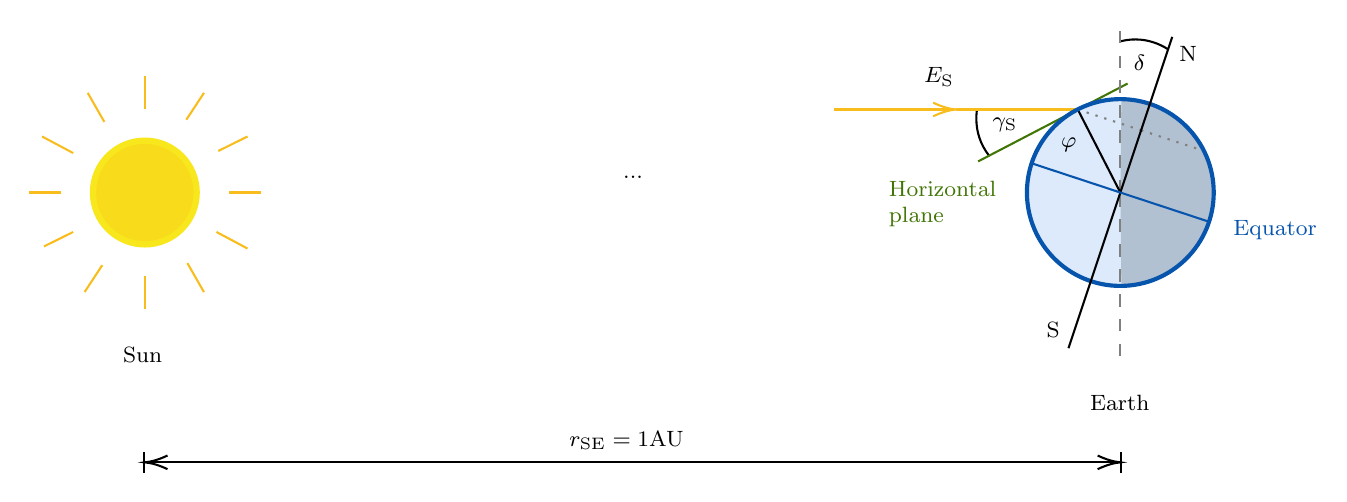
\begin{tikzpicture}[x=0.75pt,y=0.75pt,yscale=-1,xscale=1]
%uncomment if require: \path (0,447); %set diagram left start at 0, and has height of 447

%Shape: Pie [id:dp15034815819494352] 
\draw  [color={rgb, 255:red, 0; green, 0; blue, 0 }  ,draw opacity=0 ][fill={rgb, 255:red, 0; green, 0; blue, 0 }  ,fill opacity=0.45 ] (545.51,179.99) .. controls (570.29,180.26) and (590.33,200.21) .. (590.41,224.85) .. controls (590.49,249.59) and (570.42,269.74) .. (545.5,270.01) -- (545,225) -- cycle ;
%Shape: Circle [id:dp11400902817768599] 
\draw  [color={rgb, 255:red, 7; green, 84; blue, 173 }  ,draw opacity=1 ][fill={rgb, 255:red, 200; green, 222; blue, 248 }  ,fill opacity=0.64 ][line width=0.75]  (500,225) .. controls (500,200.15) and (520.15,180) .. (545,180) .. controls (569.85,180) and (590,200.15) .. (590,225) .. controls (590,249.85) and (569.85,270) .. (545,270) .. controls (520.15,270) and (500,249.85) .. (500,225) -- cycle ;
%Straight Lines [id:da48130102628083926] 
\draw [color={rgb, 255:red, 65; green, 117; blue, 5 }  ,draw opacity=1 ]   (548.5,172.5) -- (524.5,185) ;
%Shape: Arc [id:dp6322515277427461] 
\draw  [draw opacity=0] (481.9,207.42) .. controls (480.77,206.02) and (479.77,204.5) .. (478.91,202.87) .. controls (475.99,197.34) and (475.08,191.17) .. (475.92,184.97) -- (518.5,182) -- cycle ; \draw   (481.9,207.42) .. controls (480.77,206.02) and (479.77,204.5) .. (478.91,202.87) .. controls (475.99,197.34) and (475.08,191.17) .. (475.92,184.97) ;
%Straight Lines [id:da15968904032085707] 
\draw [color={rgb, 255:red, 65; green, 117; blue, 5 }  ,draw opacity=1 ]   (476.5,210) -- (524.5,185) ;
%Shape: Circle [id:dp68849801426956] 
\draw  [color={rgb, 255:red, 248; green, 231; blue, 28 }  ,draw opacity=1 ][fill={rgb, 255:red, 248; green, 220; blue, 28 }  ,fill opacity=1 ][line width=2.25]  (50,225) .. controls (50,211.19) and (61.19,200) .. (75,200) .. controls (88.81,200) and (100,211.19) .. (100,225) .. controls (100,238.81) and (88.81,250) .. (75,250) .. controls (61.19,250) and (50,238.81) .. (50,225) -- cycle ;
%Shape: Arc [id:dp11190386681659015] 
\draw  [draw opacity=0] (544.71,152.26) .. controls (547.24,151.56) and (549.86,151.21) .. (552.55,151.25) .. controls (558.14,151.31) and (563.41,153.04) .. (568.08,156.04) -- (552,196) -- cycle ; \draw   (544.71,152.26) .. controls (547.24,151.56) and (549.86,151.21) .. (552.55,151.25) .. controls (558.14,151.31) and (563.41,153.04) .. (568.08,156.04) ;
%Straight Lines [id:da09161822286264387] 
\draw [color={rgb, 255:red, 128; green, 128; blue, 128 }  ,draw opacity=1 ] [dash pattern={on 4.5pt off 4.5pt}]  (545,303.92) -- (545,225) ;
%Straight Lines [id:da48620147126216584] 
\draw [color={rgb, 255:red, 128; green, 128; blue, 128 }  ,draw opacity=1 ] [dash pattern={on 4.5pt off 4.5pt}]  (545,225) -- (545,146.08) ;
%Straight Lines [id:da2344822206483721] 
\draw [line width=0.75]    (524.5,185) -- (545,225) ;
%Straight Lines [id:da23327222270661996] 
\draw    (77,355) -- (543,355) ;
\draw [shift={(545,355)}, rotate = 180] [color={rgb, 255:red, 0; green, 0; blue, 0 }  ][line width=0.75]    (10.93,-3.29) .. controls (6.95,-1.4) and (3.31,-0.3) .. (0,0) .. controls (3.31,0.3) and (6.95,1.4) .. (10.93,3.29)   ;
\draw [shift={(75,355)}, rotate = 0] [color={rgb, 255:red, 0; green, 0; blue, 0 }  ][line width=0.75]    (10.93,-3.29) .. controls (6.95,-1.4) and (3.31,-0.3) .. (0,0) .. controls (3.31,0.3) and (6.95,1.4) .. (10.93,3.29)   ;
%Straight Lines [id:da6929947931128337] 
\draw [color={rgb, 255:red, 248; green, 189; blue, 28 }  ,draw opacity=1 ]   (407,185) -- (463.75,185) ;
\draw [shift={(465.75,185)}, rotate = 180] [color={rgb, 255:red, 248; green, 189; blue, 28 }  ,draw opacity=1 ][line width=0.75]    (10.93,-3.29) .. controls (6.95,-1.4) and (3.31,-0.3) .. (0,0) .. controls (3.31,0.3) and (6.95,1.4) .. (10.93,3.29)   ;
%Straight Lines [id:da9358361305294991] 
\draw [color={rgb, 255:red, 248; green, 189; blue, 28 }  ,draw opacity=1 ]   (524.5,185) -- (465.75,185) ;
%Straight Lines [id:da7529976931050752] 
\draw    (545.5,350) -- (545.5,360) ;
%Straight Lines [id:da4019381676598568] 
\draw [color={rgb, 255:red, 128; green, 128; blue, 128 }  ,draw opacity=1 ] [dash pattern={on 0.84pt off 2.51pt}]  (555,195) -- (585.5,205) ;
%Straight Lines [id:da051171793746800365] 
\draw [color={rgb, 255:red, 128; green, 128; blue, 128 }  ,draw opacity=1 ] [dash pattern={on 0.84pt off 2.51pt}]  (524.5,185) -- (555,195) ;
%Shape: Circle [id:dp6054942149883367] 
\draw  [color={rgb, 255:red, 7; green, 84; blue, 173 }  ,draw opacity=1 ][fill={rgb, 255:red, 200; green, 222; blue, 248 }  ,fill opacity=0 ][line width=1.5]  (500,225) .. controls (500,200.15) and (520.15,180) .. (545,180) .. controls (569.85,180) and (590,200.15) .. (590,225) .. controls (590,249.85) and (569.85,270) .. (545,270) .. controls (520.15,270) and (500,249.85) .. (500,225) -- cycle ;
%Straight Lines [id:da7513058172554794] 
\draw    (545,225) -- (520,300) ;
%Straight Lines [id:da456675238429898] 
\draw    (570,150) -- (545,225) ;
%Straight Lines [id:da7902385793672442] 
\draw [color={rgb, 255:red, 7; green, 84; blue, 173 }  ,draw opacity=1 ]   (502.5,211) -- (545,225) ;
%Straight Lines [id:da2311496114593583] 
\draw [color={rgb, 255:red, 7; green, 84; blue, 173 }  ,draw opacity=1 ]   (545,225) -- (587.5,239) ;
%Straight Lines [id:da7859324779499595] 
\draw [color={rgb, 255:red, 248; green, 189; blue, 28 }  ,draw opacity=1 ]   (75,169.06) -- (75,184.63) ;
%Straight Lines [id:da6628690922559444] 
\draw [color={rgb, 255:red, 248; green, 189; blue, 28 }  ,draw opacity=1 ]   (130.94,225) -- (115.38,225) ;
%Straight Lines [id:da059104507396427586] 
\draw [color={rgb, 255:red, 248; green, 189; blue, 28 }  ,draw opacity=1 ]   (75,280.94) -- (75,265.38) ;
%Straight Lines [id:da13924610653156622] 
\draw [color={rgb, 255:red, 248; green, 189; blue, 28 }  ,draw opacity=1 ]   (34.63,225) -- (19.06,225) ;
%Straight Lines [id:da6612538806605628] 
\draw [color={rgb, 255:red, 248; green, 189; blue, 28 }  ,draw opacity=1 ]   (109.5,244) -- (124.5,252) ;
%Straight Lines [id:da6313529241657796] 
\draw [color={rgb, 255:red, 248; green, 189; blue, 28 }  ,draw opacity=1 ]   (25.5,198) -- (40.5,206) ;
%Straight Lines [id:da5019670096718076] 
\draw [color={rgb, 255:red, 248; green, 189; blue, 28 }  ,draw opacity=1 ]   (124.5,198) -- (110.38,205) ;
%Straight Lines [id:da9267861672263464] 
\draw [color={rgb, 255:red, 248; green, 189; blue, 28 }  ,draw opacity=1 ]   (40.5,244) -- (26.38,251) ;
%Straight Lines [id:da8979247612603714] 
\draw [color={rgb, 255:red, 248; green, 189; blue, 28 }  ,draw opacity=1 ]   (95,189.94) -- (103.5,177) ;
%Straight Lines [id:da4019503947575047] 
\draw [color={rgb, 255:red, 248; green, 189; blue, 28 }  ,draw opacity=1 ]   (46,272.94) -- (54.5,260) ;
%Straight Lines [id:da27205273028090327] 
\draw [color={rgb, 255:red, 248; green, 189; blue, 28 }  ,draw opacity=1 ]   (95.5,259) -- (103.5,273) ;
%Straight Lines [id:da5079939363345163] 
\draw [color={rgb, 255:red, 248; green, 189; blue, 28 }  ,draw opacity=1 ]   (47.5,177) -- (55.5,191) ;
%Straight Lines [id:da7553342413027122] 
\draw    (74.5,360) -- (74.5,350) ;

% Text Node
\draw (515,197.4) node [anchor=north west][inner sep=0.75pt]  [font=\footnotesize]  {$\varphi $};
% Text Node
\draw (63,298) node [anchor=north west][inner sep=0.75pt]  [font=\footnotesize] [align=left] {Sun};
% Text Node
\draw (529,321) node [anchor=north west][inner sep=0.75pt]  [font=\footnotesize] [align=left] {Earth};
% Text Node
\draw (550,157.4) node [anchor=north west][inner sep=0.75pt]  [font=\footnotesize]  {$\delta $};
% Text Node
\draw (598,237) node [anchor=north west][inner sep=0.75pt]  [font=\footnotesize,color={rgb, 255:red, 7; green, 84; blue, 173 }  ,opacity=1 ] [align=left] {Equator};
% Text Node
\draw (482,187.4) node [anchor=north west][inner sep=0.75pt]  [font=\footnotesize]  {$\gamma _{\mathrm{S}}$};
% Text Node
\draw (432,218) node [anchor=north west][inner sep=0.75pt]  [font=\footnotesize,color={rgb, 255:red, 65; green, 117; blue, 5 }  ,opacity=1 ] [align=left] {Horizontal\\plane};
% Text Node
\draw (449,163.4) node [anchor=north west][inner sep=0.75pt]  [font=\footnotesize]  {$E_{\mathrm{S}}$};
% Text Node
\draw (278,338.4) node [anchor=north west][inner sep=0.75pt]  [font=\footnotesize]  {$r_{\mathrm{SE}} =1\mathrm{AU}$};
% Text Node
\draw (572,153) node [anchor=north west][inner sep=0.75pt]  [font=\footnotesize] [align=left] {N};
% Text Node
\draw (508,286) node [anchor=north west][inner sep=0.75pt]  [font=\footnotesize] [align=left] {S};
% Text Node
\draw (304,215.4) node [anchor=north west][inner sep=0.75pt]  [font=\footnotesize]  {$...$};


\end{tikzpicture}

	\caption{Angular relationship between the Sun and Earth. (Recreated from: \cite{Mertens:2015})}
	\label{fig:tikz_angular_relationship}
\end{figure} 

A great advantage of solar energy is that its source, the Sun, is highly predictable. This results in the fact, that the electrical energy supply of the self-sufficient voice communication system can be planned relatively well, as shown in the following subsections. In theory, it can be installed in almost any location where solar rays reach the surface of the Earth. A high modularity of \emph{photovoltaic} (PV) generators -- which are used to convert solar energy into electrical energy -- furthermore allows the system to be scaled up by connecting them in series for a higher voltage, or in parallel for a higher current. In both cases the power delivered by the connected PV generators is increased. In addition, PV generators have a very long service life of at least 30 years on Earth. This is due to their structure. Furthermore, compared to wind turbines, they do not have any moving mechanical parts which can be worn down over time. Finally, PV generators have a high power-to-weight ratio, which is prefered for mobile systems \cite{Landis:1995, Rebhan:2002, Mertens:2015}.\footnote{The self-sufficient voice communication system is referred to as mobile because the OeWF will conduct missions in different Mars analog regions on Earth, which requires it to be installed in different locations and therefore be shipped frequently.}

Basic stand-alone systems, as shown in figure \ref{fig:tikz/tikz_solar_energy_distribution}, mainly require a PV generator, a \emph{solar charging controller} (SCC) and an electrochemical energy storage device. In this case the electrochemical energy storage device is a rechargeable battery with a \emph{number of secondary cells} $N_\mathrm{SC}$ in $\left( 1 \right)$. The SCC is responsible for the charging process of the battery and the electrical supply of the load $R_\mathrm{L}$ in $\left( \Omega \right)$.
\begin{figure}[h!]
	\centering
	

\tikzset{every picture/.style={line width=0.75pt}} %set default line width to 0.75pt        

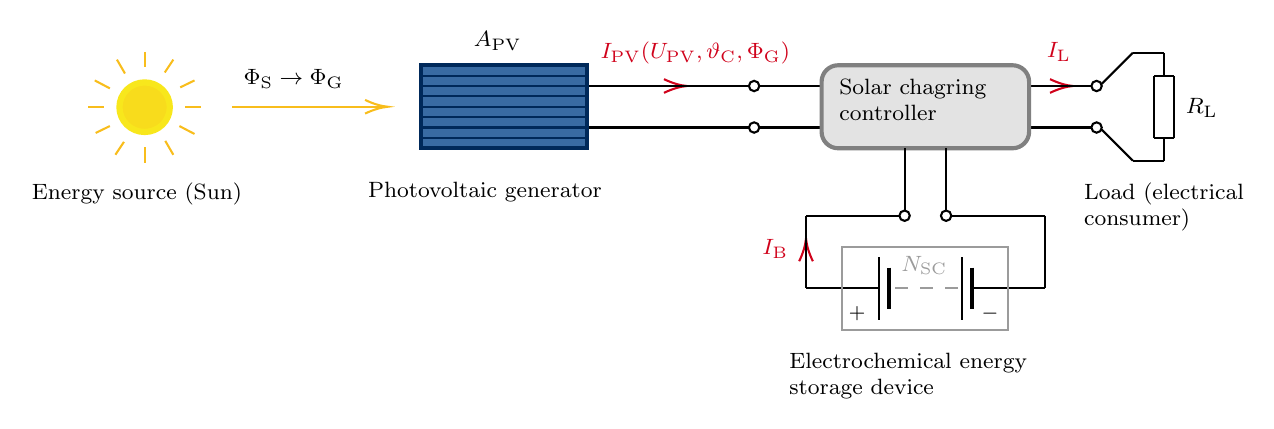
\begin{tikzpicture}[x=0.75pt,y=0.75pt,yscale=-1,xscale=1]
%uncomment if require: \path (0,411); %set diagram left start at 0, and has height of 411

%Straight Lines [id:da8136196719593345] 
\draw [color={rgb, 255:red, 208; green, 2; blue, 27 }  ,draw opacity=1 ]   (382.5,228.5) -- (382.5,215.5) ;
\draw [shift={(382.5,213.5)}, rotate = 450] [color={rgb, 255:red, 208; green, 2; blue, 27 }  ,draw opacity=1 ][line width=0.75]    (10.93,-3.29) .. controls (6.95,-1.4) and (3.31,-0.3) .. (0,0) .. controls (3.31,0.3) and (6.95,1.4) .. (10.93,3.29)   ;
%Straight Lines [id:da7467198195912443] 
\draw [color={rgb, 255:red, 208; green, 2; blue, 27 }  ,draw opacity=1 ]   (496,140) -- (509,140) ;
\draw [shift={(511,140)}, rotate = 180] [color={rgb, 255:red, 208; green, 2; blue, 27 }  ,draw opacity=1 ][line width=0.75]    (10.93,-3.29) .. controls (6.95,-1.4) and (3.31,-0.3) .. (0,0) .. controls (3.31,0.3) and (6.95,1.4) .. (10.93,3.29)   ;
%Straight Lines [id:da8214665589366665] 
\draw [color={rgb, 255:red, 208; green, 2; blue, 27 }  ,draw opacity=1 ]   (305,140) -- (323,140) ;
\draw [shift={(325,140)}, rotate = 180] [color={rgb, 255:red, 208; green, 2; blue, 27 }  ,draw opacity=1 ][line width=0.75]    (10.93,-3.29) .. controls (6.95,-1.4) and (3.31,-0.3) .. (0,0) .. controls (3.31,0.3) and (6.95,1.4) .. (10.93,3.29)   ;
%Straight Lines [id:da05884283577747018] 
\draw    (277,160) -- (355,160) ;
%Straight Lines [id:da06536461743866195] 
\draw    (277,140) -- (355,140) ;
%Shape: Ellipse [id:dp7367390116189665] 
\draw  [color={rgb, 255:red, 248; green, 231; blue, 28 }  ,draw opacity=1 ][fill={rgb, 255:red, 248; green, 220; blue, 28 }  ,fill opacity=1 ][line width=2.25]  (51.71,150.21) .. controls (51.71,143.62) and (57.15,138.27) .. (63.85,138.27) .. controls (70.55,138.27) and (75.98,143.62) .. (75.98,150.21) .. controls (75.98,156.81) and (70.55,162.15) .. (63.85,162.15) .. controls (57.15,162.15) and (51.71,156.81) .. (51.71,150.21) -- cycle ;
%Straight Lines [id:da6220717030144096] 
\draw [color={rgb, 255:red, 248; green, 189; blue, 28 }  ,draw opacity=1 ]   (63.85,123.5) -- (63.85,130.93) ;
%Straight Lines [id:da8051708851804078] 
\draw [color={rgb, 255:red, 248; green, 189; blue, 28 }  ,draw opacity=1 ]   (91,150.21) -- (83.45,150.21) ;
%Straight Lines [id:da3460695789100754] 
\draw [color={rgb, 255:red, 248; green, 189; blue, 28 }  ,draw opacity=1 ]   (63.85,176.93) -- (63.85,169.49) ;
%Straight Lines [id:da2732251675151305] 
\draw [color={rgb, 255:red, 248; green, 189; blue, 28 }  ,draw opacity=1 ]   (44.25,150.21) -- (36.7,150.21) ;
%Straight Lines [id:da4407496963374895] 
\draw [color={rgb, 255:red, 248; green, 189; blue, 28 }  ,draw opacity=1 ]   (80.59,159.29) -- (87.88,163.11) ;
%Straight Lines [id:da383911411945429] 
\draw [color={rgb, 255:red, 248; green, 189; blue, 28 }  ,draw opacity=1 ]   (39.82,137.32) -- (47.1,141.14) ;
%Straight Lines [id:da9217210977387595] 
\draw [color={rgb, 255:red, 248; green, 189; blue, 28 }  ,draw opacity=1 ]   (87.88,137.32) -- (81.02,140.66) ;
%Straight Lines [id:da03325396834222771] 
\draw [color={rgb, 255:red, 248; green, 189; blue, 28 }  ,draw opacity=1 ]   (47.1,159.29) -- (40.25,162.63) ;
%Straight Lines [id:da12285363488917289] 
\draw [color={rgb, 255:red, 248; green, 189; blue, 28 }  ,draw opacity=1 ]   (73.56,133.47) -- (77.68,127.29) ;
%Straight Lines [id:da4786379847065507] 
\draw [color={rgb, 255:red, 248; green, 189; blue, 28 }  ,draw opacity=1 ]   (49.77,173.11) -- (53.9,166.93) ;
%Straight Lines [id:da261341351601285] 
\draw [color={rgb, 255:red, 248; green, 189; blue, 28 }  ,draw opacity=1 ]   (73.8,166.45) -- (77.68,173.14) ;
%Straight Lines [id:da4643507370218185] 
\draw [color={rgb, 255:red, 248; green, 189; blue, 28 }  ,draw opacity=1 ]   (50.5,127.29) -- (54.38,133.98) ;

%Straight Lines [id:da8936580886091565] 
\draw [color={rgb, 255:red, 248; green, 189; blue, 28 }  ,draw opacity=1 ][line width=0.75]    (179,150) -- (106,150) ;
\draw [shift={(181,150)}, rotate = 180] [color={rgb, 255:red, 248; green, 189; blue, 28 }  ,draw opacity=1 ][line width=0.75]    (10.93,-3.29) .. controls (6.95,-1.4) and (3.31,-0.3) .. (0,0) .. controls (3.31,0.3) and (6.95,1.4) .. (10.93,3.29)   ;
%Shape: Circle [id:dp07158046691092301] 
\draw   (355,160) .. controls (355,158.62) and (356.12,157.5) .. (357.5,157.5) .. controls (358.88,157.5) and (360,158.62) .. (360,160) .. controls (360,161.38) and (358.88,162.5) .. (357.5,162.5) .. controls (356.12,162.5) and (355,161.38) .. (355,160) -- cycle ;
%Shape: Circle [id:dp25309308645033757] 
\draw   (355,140) .. controls (355,138.62) and (356.12,137.5) .. (357.5,137.5) .. controls (358.88,137.5) and (360,138.62) .. (360,140) .. controls (360,141.38) and (358.88,142.5) .. (357.5,142.5) .. controls (356.12,142.5) and (355,141.38) .. (355,140) -- cycle ;
%Straight Lines [id:da08781161374086754] 
\draw    (490,140) -- (520,140) ;
%Straight Lines [id:da1141924880655707] 
\draw    (490,160) -- (520,160) ;
%Shape: Circle [id:dp18646523024055295] 
\draw   (520,140) .. controls (520,138.62) and (521.12,137.5) .. (522.5,137.5) .. controls (523.88,137.5) and (525,138.62) .. (525,140) .. controls (525,141.38) and (523.88,142.5) .. (522.5,142.5) .. controls (521.12,142.5) and (520,141.38) .. (520,140) -- cycle ;
%Shape: Circle [id:dp3179313012599374] 
\draw   (520,160) .. controls (520,158.62) and (521.12,157.5) .. (522.5,157.5) .. controls (523.88,157.5) and (525,158.62) .. (525,160) .. controls (525,161.38) and (523.88,162.5) .. (522.5,162.5) .. controls (521.12,162.5) and (520,161.38) .. (520,160) -- cycle ;
%Straight Lines [id:da3754937570361223] 
\draw    (560,135) -- (550,135) ;
%Straight Lines [id:da28765380259572004] 
\draw    (560,165) -- (550,165) ;
%Straight Lines [id:da7994093769920398] 
\draw    (550,165) -- (550,135) ;
%Straight Lines [id:da49571728514760194] 
\draw    (560,165) -- (560,135) ;
%Straight Lines [id:da8708596386928309] 
\draw    (525,139) -- (540,124) ;
%Straight Lines [id:da34435901343623154] 
\draw    (360,140) -- (390,140) ;
%Straight Lines [id:da885690749449715] 
\draw    (360,160) -- (390,160) ;
%Straight Lines [id:da5154787772311555] 
\draw    (525,161) -- (540,176) ;
%Straight Lines [id:da8283908147650987] 
\draw    (540,124) -- (555,124) ;
%Straight Lines [id:da576788078319086] 
\draw    (540,176) -- (555,176) ;
%Straight Lines [id:da1720155229910998] 
\draw    (555,124) -- (555,135) ;
%Straight Lines [id:da2995787552008038] 
\draw    (555,165) -- (555,176) ;
%Rounded Rect [id:dp605862839350801] 
\draw  [color={rgb, 255:red, 128; green, 128; blue, 128 }  ,draw opacity=1 ][fill={rgb, 255:red, 227; green, 227; blue, 227 }  ,fill opacity=1 ][line width=1.5]  (390,138) .. controls (390,133.58) and (393.58,130) .. (398,130) -- (482,130) .. controls (486.42,130) and (490,133.58) .. (490,138) -- (490,162) .. controls (490,166.42) and (486.42,170) .. (482,170) -- (398,170) .. controls (393.58,170) and (390,166.42) .. (390,162) -- cycle ;
%Shape: Rectangle [id:dp22380146308476956] 
\draw  [color={rgb, 255:red, 0; green, 41; blue, 90 }  ,draw opacity=1 ][fill={rgb, 255:red, 57; green, 107; blue, 163 }  ,fill opacity=1 ][line width=1.5]  (197,130) -- (277,130) -- (277,170) -- (197,170) -- cycle ;
%Straight Lines [id:da2633344010900689] 
\draw [color={rgb, 255:red, 0; green, 41; blue, 90 }  ,draw opacity=1 ]   (197,135) -- (277,135) ;
%Straight Lines [id:da7329634137016672] 
\draw [color={rgb, 255:red, 0; green, 41; blue, 90 }  ,draw opacity=1 ]   (197,140) -- (277,140) ;
%Straight Lines [id:da3363363364783303] 
\draw [color={rgb, 255:red, 0; green, 41; blue, 90 }  ,draw opacity=1 ]   (197,150) -- (277,150) ;
%Straight Lines [id:da5631412852438793] 
\draw [color={rgb, 255:red, 0; green, 41; blue, 90 }  ,draw opacity=1 ]   (197,145) -- (277,145) ;
%Straight Lines [id:da6153878400696737] 
\draw [color={rgb, 255:red, 0; green, 41; blue, 90 }  ,draw opacity=1 ]   (197,155) -- (277,155) ;
%Straight Lines [id:da7384152042955765] 
\draw [color={rgb, 255:red, 0; green, 41; blue, 90 }  ,draw opacity=1 ]   (197,160) -- (277,160) ;
%Straight Lines [id:da4382619041484126] 
\draw [color={rgb, 255:red, 0; green, 41; blue, 90 }  ,draw opacity=1 ]   (197,165) -- (277,165) ;

%Straight Lines [id:da3400420847168515] 
\draw    (450,170) -- (450,200) ;
%Straight Lines [id:da6795701825095302] 
\draw    (430,170) -- (430,200) ;

%Shape: Circle [id:dp030153076038484272] 
\draw   (447.5,202.5) .. controls (447.5,201.12) and (448.62,200) .. (450,200) .. controls (451.38,200) and (452.5,201.12) .. (452.5,202.5) .. controls (452.5,203.88) and (451.38,205) .. (450,205) .. controls (448.62,205) and (447.5,203.88) .. (447.5,202.5) -- cycle ;
%Shape: Circle [id:dp08428574429470248] 
\draw   (427.5,202.5) .. controls (427.5,201.12) and (428.62,200) .. (430,200) .. controls (431.38,200) and (432.5,201.12) .. (432.5,202.5) .. controls (432.5,203.88) and (431.38,205) .. (430,205) .. controls (428.62,205) and (427.5,203.88) .. (427.5,202.5) -- cycle ;
%Straight Lines [id:da024547296314676226] 
\draw    (402.5,237.5) -- (382.5,237.5) ;
%Straight Lines [id:da8993285949308742] 
\draw [line width=0.75]    (417.5,222.5) -- (417.5,252.5) ;
%Straight Lines [id:da9178918649128838] 
\draw [color={rgb, 255:red, 155; green, 155; blue, 155 }  ,draw opacity=1 ] [dash pattern={on 4.5pt off 4.5pt}]  (455.5,237.5) -- (420.5,237.5) ;
%Straight Lines [id:da3598630804907186] 
\draw [line width=1.5]    (422.5,227.5) -- (422.5,247.5) ;
%Straight Lines [id:da4254329027835011] 
\draw [line width=0.75]    (457.5,222.5) -- (457.5,252.5) ;
%Straight Lines [id:da7513947415530464] 
\draw [line width=1.5]    (462.5,227.5) -- (462.5,247.5) ;
%Straight Lines [id:da24748868677387104] 
\draw    (417.5,237.5) -- (402.5,237.5) ;
%Straight Lines [id:da009805082115965202] 
\draw    (477.5,237.5) -- (462.5,237.5) ;
%Straight Lines [id:da7428727764436842] 
\draw    (497.5,237.5) -- (477.5,237.5) ;
%Shape: Rectangle [id:dp13613803613375608] 
\draw  [color={rgb, 255:red, 155; green, 155; blue, 155 }  ,draw opacity=1 ] (480,217.5) -- (480,257.5) -- (400,257.5) -- (400,217.5) -- cycle ;
%Straight Lines [id:da9313000955522079] 
\draw    (452.5,202.5) -- (497.5,202.5) ;
%Straight Lines [id:da4244913203234748] 
\draw    (382.5,202.5) -- (427.5,202.5) ;
%Straight Lines [id:da11099998272282585] 
\draw    (382.5,202.5) -- (382.5,237.5) ;
%Straight Lines [id:da2340928507704263] 
\draw    (497.5,202.5) -- (497.5,237.5) ;

% Text Node
\draw (8,185) node [anchor=north west][inner sep=0.75pt]  [font=\footnotesize] [align=left] {Energy source (Sun)};
% Text Node
\draw (170,185) node [anchor=north west][inner sep=0.75pt]  [font=\footnotesize] [align=left] {Photovoltaic generator};
% Text Node
\draw (110,130.4) node [anchor=north west][inner sep=0.75pt]  [font=\footnotesize]  {$\Phi _{\mathrm{S}}\rightarrow \Phi _{\mathrm{G}}$};
% Text Node
\draw (282,117.4) node [anchor=north west][inner sep=0.75pt]  [font=\footnotesize,color={rgb, 255:red, 208; green, 2; blue, 27 }  ,opacity=1 ]  {$I_{\mathrm{PV}}( U_{\mathrm{PV}} ,\vartheta _{\mathrm{C}} ,\Phi _{\mathrm{G}})$};
% Text Node
\draw (397.08,135) node [anchor=north west][inner sep=0.75pt]  [font=\footnotesize] [align=left] {Solar chagring\\controller};
% Text Node
\draw (515,185) node [anchor=north west][inner sep=0.75pt]  [font=\footnotesize] [align=left] {Load (electrical \\consumer)};
% Text Node
\draw (497,117.4) node [anchor=north west][inner sep=0.75pt]  [font=\footnotesize,color={rgb, 255:red, 208; green, 2; blue, 27 }  ,opacity=1 ]  {$I_{\mathrm{L}}$};
% Text Node
\draw (401.5,244.9) node [anchor=north west][inner sep=0.75pt]  [font=\scriptsize]  {$+$};
% Text Node
\draw (465.5,244.9) node [anchor=north west][inner sep=0.75pt]  [font=\scriptsize]  {$-$};
% Text Node
\draw (427,220.4) node [anchor=north west][inner sep=0.75pt]  [font=\footnotesize,color={rgb, 255:red, 155; green, 155; blue, 155 }  ,opacity=1 ]  {$N_{\mathrm{SC}}$};
% Text Node
\draw (360,212.4) node [anchor=north west][inner sep=0.75pt]  [font=\footnotesize,color={rgb, 255:red, 208; green, 2; blue, 27 }  ,opacity=1 ]  {$I_{\mathrm{B}}$};
% Text Node
\draw (373,267) node [anchor=north west][inner sep=0.75pt]  [font=\footnotesize] [align=left] {Electrochemical energy\\storage device};
% Text Node
\draw (564,144.4) node [anchor=north west][inner sep=0.75pt]  [font=\footnotesize]  {$R_{\mathrm{L}}$};
% Text Node
\draw (221,112.4) node [anchor=north west][inner sep=0.75pt]  [font=\footnotesize]  {$A_{\mathrm{PV}}$};


\end{tikzpicture}

	\caption{Basic structure of an electrical stand-alone system which is supplied with electrical energy by a photovoltaic generator. The energy is stored in an electrochemical energy storage device.}
	\label{fig:tikz/tikz_solar_energy_distribution}
\end{figure}
As illustrated in figure \ref{fig:tikz/tikz_solar_energy_distribution}, the radiation flux $\Phi_{\mathrm{G}}$ in $\left( \mathrm{W} \right)$ onto the PV generator's \emph{energy-converting area} $A_{\mathrm{PV}}$ in $\left( \mathrm{m}^2 \right)$ can be converted into electrical energy. This results in the \emph{PV generator current} $I_{\mathrm{PV}}\left( U_{\mathrm{PV}}, \vartheta_\mathrm{C}, \Phi_\mathrm{G} \right)$ in $\left( \mathrm{A} \right)$. In addition to the radiation flux $\Phi_\mathrm{G}$, this current depends on the \emph{PV generator voltage}\footnote{$I_{\mathrm{PV}}\left( U_{\mathrm{PV}} \right)$ defines the current-voltage characteristic of a PV generator.} $U_{\mathrm{PV}}$ in $\left( \mathrm{V} \right)$ and the \emph{temperature} of the PV cells -- of which the PV generator consists -- $\vartheta_{\mathrm{C}}$ in $\left( ^\circ \mathrm{C} \right)$, as this temperature plays an important role in the power output of a PV generator. For both, the PV generator and the load, the upper electrical connection (circle) represents the positive electric potential, from which the reference directions for the electrical currents directly follow. $I_\mathrm{B}$ in $\left( \mathrm{A}\right)$ is the \emph{battery current} and $I_\mathrm{L}$ in $\left( \mathrm{A}\right)$ is the \emph{load current}. \cite{Ley:2011, Bertol:2011, Mertens:2015}.

With regard to future Mars missions the authors of the articles \cite{Appelbaum:1990, Appelbaum:1992, Landis:1995} found out, that even during prolonged Martian dust storms -- when the Martian atmosphere becomes almost opaque -- a PV generator could still convert electrical energy, due to the diffuse component of sunlight. This is suppored by empirical data measured with PV generators on Earth as shown in the book \cite{Mertens:2015} and by solar resource maps for Earth's surface provided by \cite{SolargisMaps:2020, GlobalSolarAtlas:2020, Union:2020}. The authors of the article \cite[1]{Landis:1995} furthermore state: \textit{``Solar energy is likely to be an important power source for surface-bound operations on Mars.''}, which is another reason why solar energy was selected as a renewable energy source to supply the self-sufficient voice communication system.

In the following subsections the modeling of the self-sufficient energy distribution system of the voice communication system on Earth will be explained. The last subsection adapts these findings to a Martian application. % Change this if necessary

% Subsections:
\subsection{Angular relationships} \label{sec:angular_relationships}
Before the energy yield of a PV generator can be calculated, it is essential to introduce a few important angles -- of which some were already mentioned -- and define how they are counted in this thesis.

The local latitude $\varphi$ at the equator is $0^\circ$ and it is counted positive towards the north and negative towards the south with a range of $\left[-90^\circ \text{, } 90^\circ\right]$, and the local \emph{longitude} $\lambda$ in $\left(^\circ\right)$ is $0^\circ$ at the reference meridian $\lambda_0$ in $\left(^\circ\right)$ which passes through the Greenwich Observatory in the United Kingdom. $\lambda$ is counted positive east and negative west of Greenwich with a range of $\left(-180^\circ \text{, } 180^\circ\right]$ \cite{Landis:1995, Karttunen:2006, Wagner:2018}. For completens it should be mentioned that the latitude $\varphi$ and the longitude $\lambda$ -- for a given location on Earth -- can be obtained from an atlas or a \emph{global positioning system} (GPS) device.

The Sun's declination $\delta$ indicates how far the Earth's axis of rotations -- which runs through the North and South Poles -- leans towards the Sun at solar noon. Its range is $\left[-90^\circ \text{, } 90^\circ\right]$, although its maximum values for Earth are $-23,45^\circ$ and $23,45^\circ$. $\delta$ is counted negative if the North Pole leans away from the Sun and positive if it leans towards the Sun (compare to figure \ref{fig:tikz_angular_relationship}) \cite{Landis:1995, Karttunen:2006, Mertens:2015, Wagner:2018}. As per \cite{Wagner:2018}, the following approximation for $\delta$ at a given day of the year, with $N_d$ being the \emph{number of days} since January 1\textsuperscript{st} in $\left(\mathrm d \right)$,  $mon$ being the \emph{month} in $\left( 1 \right)$ and $d$ being the \emph{day} in $\left(\mathrm d \right)$, is sufficient for photovoltaic applications: 
	\begin{equation} \label{eq:delta}
	\centering
		\delta \approx 23,45^\circ \cdot \sin \left(360^\circ \cdot \frac{284\mathrm{d} + N_d}{365\mathrm{d}}\right) \text{,} 
	\end{equation}
	\begin{equation} \label{eq:delta}
	\centering
		N_d \approx 30,3\mathrm{d} \cdot \left(mon - 1\right) + d \text{.}
	\end{equation}

The altitude $\gamma_{\mathrm{S}}$ and the \emph{azimuth} $\alpha_{\mathrm{S}}$ of the Sun in $\left(^\circ \right)$, presented in the equations (\ref{eq:sin_gamma_s}) and (\ref{eq:cos_alpha_s}), describe its position in the sky over the course of the day, with $\gamma_{\mathrm{S}}$ taking on values within $\left[0^\circ \text{, } 90^\circ\right]$ and $\alpha_{\mathrm{S}}$ taking on values within $\left(-180^\circ \text{, } 180^\circ \right]$. How these angles are measured -- with the corresponding celstial hemisphere of an observer -- is shown in the figure \ref{fig:tikz_gamma_s_alpha_s}. For $\gamma_{\mathrm{S}} = 0^\circ$ the Sun is visible at the horizon and for $\gamma_{\mathrm{S}} = 90^\circ$ it is visible at its zenith. For $\alpha_{\mathrm{S}} = 0^\circ$ the Sun is visible exactly in the south. $\alpha_{\mathrm{S}}$ takes on positive values towards the west and negative values towards the east \cite{Landis:1995, Karttunen:2006, Mertens:2015, Wagner:2018}.
	\begin{equation} \label{eq:sin_gamma_s}
	\centering
		\sin \gamma_{\mathrm{S}} = \sin \varphi \, \sin \delta + \cos \varphi \, \cos \delta \, \cos h_{\mathrm{S}}
	\end{equation}
	\begin{equation} \label{eq:cos_alpha_s}
	\centering
		\cos \alpha_{\mathrm{S}} = \frac{\sin \varphi \, \cos \delta \, \cos h_{\mathrm{S}} - \cos \varphi \, \sin \delta}{\cos \gamma_{\mathrm{S}}}
	\end{equation}
\begin{figure}[h!]
	\centering
	

\tikzset{every picture/.style={line width=0.75pt}} %set default line width to 0.75pt        

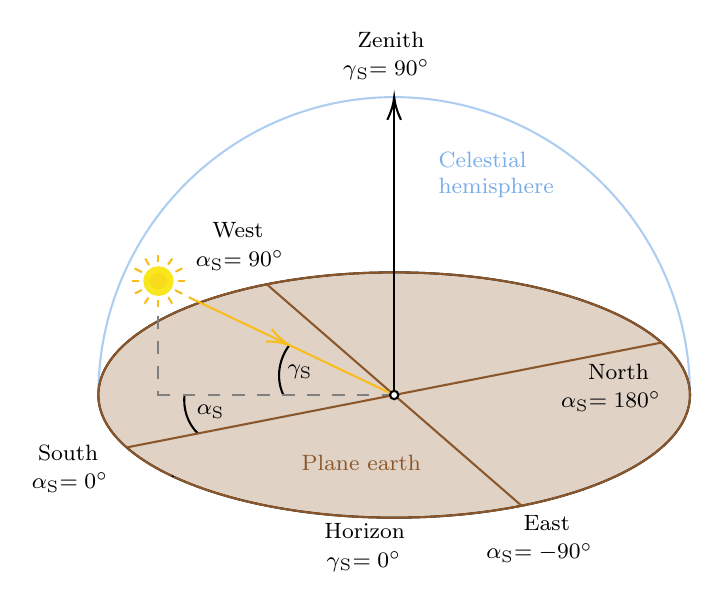
\begin{tikzpicture}[x=0.75pt,y=0.75pt,yscale=-1,xscale=1]
%uncomment if require: \path (0,445); %set diagram left start at 0, and has height of 445






%Shape: Ellipse [id:dp10248886204350427] 
\draw  [color={rgb, 255:red, 0; green, 0; blue, 0 }  ,draw opacity=1 ][fill={rgb, 255:red, 139; green, 87; blue, 42 }  ,fill opacity=0.27 ] (120.55,216.48) .. controls (120.55,183.84) and (184.36,157.39) .. (263.08,157.39) .. controls (341.79,157.39) and (405.61,183.84) .. (405.61,216.48) .. controls (405.61,249.12) and (341.79,275.58) .. (263.08,275.58) .. controls (184.36,275.58) and (120.55,249.12) .. (120.55,216.48) -- cycle ;
%Shape: Arc [id:dp9824695676563142] 
\draw  [draw opacity=0] (120.55,216.48) .. controls (120.55,216.48) and (120.55,216.48) .. (120.55,216.48) .. controls (120.55,137.22) and (184.36,72.96) .. (263.08,72.96) .. controls (341.79,72.96) and (405.61,137.22) .. (405.61,216.48) -- (263.08,216.48) -- cycle ; \draw  [color={rgb, 255:red, 74; green, 144; blue, 226 }  ,draw opacity=0.45 ] (120.55,216.48) .. controls (120.55,216.48) and (120.55,216.48) .. (120.55,216.48) .. controls (120.55,137.22) and (184.36,72.96) .. (263.08,72.96) .. controls (341.79,72.96) and (405.61,137.22) .. (405.61,216.48) ;
%Shape: Ellipse [id:dp6726138734461271] 
\draw  [color={rgb, 255:red, 248; green, 231; blue, 28 }  ,draw opacity=1 ][fill={rgb, 255:red, 248; green, 220; blue, 28 }  ,fill opacity=1 ][line width=2.25]  (143.71,161.61) .. controls (143.71,158.48) and (146.3,155.95) .. (149.5,155.95) .. controls (152.7,155.95) and (155.3,158.48) .. (155.3,161.61) .. controls (155.3,164.73) and (152.7,167.27) .. (149.5,167.27) .. controls (146.3,167.27) and (143.71,164.73) .. (143.71,161.61) -- cycle ;
%Straight Lines [id:da22837958638990763] 
\draw [color={rgb, 255:red, 248; green, 189; blue, 28 }  ,draw opacity=1 ]   (149.5,148.94) -- (149.5,152.47) ;
%Straight Lines [id:da36410436567305116] 
\draw [color={rgb, 255:red, 248; green, 189; blue, 28 }  ,draw opacity=1 ]   (162.47,161.61) -- (158.86,161.61) ;
%Straight Lines [id:da7784535438011968] 
\draw [color={rgb, 255:red, 248; green, 189; blue, 28 }  ,draw opacity=1 ]   (149.5,174.27) -- (149.5,170.75) ;
%Straight Lines [id:da02148874103533327] 
\draw [color={rgb, 255:red, 248; green, 189; blue, 28 }  ,draw opacity=1 ]   (140.14,161.61) -- (136.53,161.61) ;
%Straight Lines [id:da5806655094182651] 
\draw [color={rgb, 255:red, 248; green, 189; blue, 28 }  ,draw opacity=1 ]   (157.5,165.91) -- (160.98,167.72) ;
%Straight Lines [id:da9042107417993022] 
\draw [color={rgb, 255:red, 248; green, 189; blue, 28 }  ,draw opacity=1 ]   (138.03,155.49) -- (141.5,157.31) ;
%Straight Lines [id:da8739850131703888] 
\draw [color={rgb, 255:red, 248; green, 189; blue, 28 }  ,draw opacity=1 ]   (160.98,155.49) -- (157.7,157.08) ;
%Straight Lines [id:da9973855947966144] 
\draw [color={rgb, 255:red, 248; green, 189; blue, 28 }  ,draw opacity=1 ]   (141.5,165.91) -- (138.23,167.49) ;
%Straight Lines [id:da23606504338204548] 
\draw [color={rgb, 255:red, 248; green, 189; blue, 28 }  ,draw opacity=1 ]   (154.14,153.67) -- (156.11,150.74) ;
%Straight Lines [id:da06728456263139648] 
\draw [color={rgb, 255:red, 248; green, 189; blue, 28 }  ,draw opacity=1 ]   (142.78,172.46) -- (144.75,169.53) ;
%Straight Lines [id:da5070173352082208] 
\draw [color={rgb, 255:red, 248; green, 189; blue, 28 }  ,draw opacity=1 ]   (154.26,169.3) -- (156.11,172.47) ;
%Straight Lines [id:da536701929565258] 
\draw [color={rgb, 255:red, 248; green, 189; blue, 28 }  ,draw opacity=1 ]   (143.13,150.74) -- (144.98,153.91) ;
%Straight Lines [id:da1832197332832679] 
\draw [color={rgb, 255:red, 139; green, 87; blue, 42 }  ,draw opacity=1 ]   (324.28,269.67) -- (263.08,216.48) ;
%Straight Lines [id:da35722852927602045] 
\draw [color={rgb, 255:red, 139; green, 87; blue, 42 }  ,draw opacity=1 ]   (263.08,216.48) -- (201.88,163.3) ;
%Shape: Arc [id:dp6576066040432391] 
\draw  [draw opacity=0] (168.58,235.07) .. controls (163.53,230.23) and (161.29,223.2) .. (162.06,216.13) -- (185.16,216.91) -- cycle ; \draw   (168.58,235.07) .. controls (163.53,230.23) and (161.29,223.2) .. (162.06,216.13) ;
%Shape: Arc [id:dp8644885498360859] 
\draw  [draw opacity=0] (209.82,216.7) .. controls (206.04,209.04) and (207.21,199.65) .. (212.57,192.43) -- (231.46,205.17) -- cycle ; \draw   (209.82,216.7) .. controls (206.04,209.04) and (207.21,199.65) .. (212.57,192.43) ;
%Straight Lines [id:da40176543382530383] 
\draw [color={rgb, 255:red, 248; green, 189; blue, 28 }  ,draw opacity=1 ]   (263.08,216.48) -- (212.58,192.42) ;
%Straight Lines [id:da43066607290523007] 
\draw [color={rgb, 255:red, 128; green, 128; blue, 128 }  ,draw opacity=1 ] [dash pattern={on 4.5pt off 4.5pt}]  (149.15,216.48) -- (263.08,216.48) ;
%Straight Lines [id:da9460200323685761] 
\draw [color={rgb, 255:red, 139; green, 87; blue, 42 }  ,draw opacity=1 ]   (133.86,241.81) -- (263.08,216.48) ;
%Straight Lines [id:da12611331746579268] 
\draw [color={rgb, 255:red, 139; green, 87; blue, 42 }  ,draw opacity=1 ]   (263.08,216.48) -- (392.3,191.15) ;
%Shape: Arc [id:dp7682340536128898] 
\draw  [draw opacity=0] (155.96,255.47) .. controls (133.92,245.06) and (120.55,231.42) .. (120.55,216.48) .. controls (120.55,183.84) and (184.36,157.39) .. (263.08,157.39) .. controls (341.79,157.39) and (405.61,183.84) .. (405.61,216.48) .. controls (405.61,249.12) and (341.79,275.58) .. (263.08,275.58) .. controls (220.87,275.58) and (182.95,267.97) .. (156.85,255.88) -- (263.08,216.48) -- cycle ; \draw  [color={rgb, 255:red, 139; green, 87; blue, 42 }  ,draw opacity=1 ] (155.96,255.47) .. controls (133.92,245.06) and (120.55,231.42) .. (120.55,216.48) .. controls (120.55,183.84) and (184.36,157.39) .. (263.08,157.39) .. controls (341.79,157.39) and (405.61,183.84) .. (405.61,216.48) .. controls (405.61,249.12) and (341.79,275.58) .. (263.08,275.58) .. controls (220.87,275.58) and (182.95,267.97) .. (156.85,255.88) ;
%Straight Lines [id:da15722411504245715] 
\draw [color={rgb, 255:red, 128; green, 128; blue, 128 }  ,draw opacity=1 ] [dash pattern={on 4.5pt off 4.5pt}]  (149.5,178.56) -- (149.5,216.93) ;
%Straight Lines [id:da003502427569964439] 
\draw [color={rgb, 255:red, 248; green, 189; blue, 28 }  ,draw opacity=1 ]   (210.77,191.57) -- (164.08,169.36) ;
\draw [shift={(212.57,192.43)}, rotate = 205.44] [color={rgb, 255:red, 248; green, 189; blue, 28 }  ,draw opacity=1 ][line width=0.75]    (10.93,-3.29) .. controls (6.95,-1.4) and (3.31,-0.3) .. (0,0) .. controls (3.31,0.3) and (6.95,1.4) .. (10.93,3.29)   ;
%Straight Lines [id:da8840339574734517] 
\draw    (263.08,216.48) -- (263.08,74.96) ;
\draw [shift={(263.08,72.96)}, rotate = 450] [color={rgb, 255:red, 0; green, 0; blue, 0 }  ][line width=0.75]    (10.93,-3.29) .. controls (6.95,-1.4) and (3.31,-0.3) .. (0,0) .. controls (3.31,0.3) and (6.95,1.4) .. (10.93,3.29)   ;
%Shape: Circle [id:dp5710959149747352] 
\draw  [fill={rgb, 255:red, 255; green, 255; blue, 255 }  ,fill opacity=1 ] (261.08,216.48) .. controls (261.08,215.38) and (261.97,214.48) .. (263.08,214.48) .. controls (264.18,214.48) and (265.08,215.38) .. (265.08,216.48) .. controls (265.08,217.59) and (264.18,218.48) .. (263.08,218.48) .. controls (261.97,218.48) and (261.08,217.59) .. (261.08,216.48) -- cycle ;

% Text Node
\draw (210.29,200.68) node [anchor=north west][inner sep=0.75pt]  [font=\footnotesize]  {$\gamma _{\mathrm{S}}$};
% Text Node
\draw (166.49,219.8) node [anchor=north west][inner sep=0.75pt]  [font=\footnotesize]  {$\alpha _{\mathrm{S}}$};
% Text Node
\draw (217,244) node [anchor=north west][inner sep=0.75pt]  [font=\footnotesize,color={rgb, 255:red, 139; green, 87; blue, 42 }  ,opacity=1 ] [align=left] {Plane earth};
% Text Node
\draw (87,252.4) node [anchor=north west][inner sep=0.75pt]  [font=\footnotesize]  {$\textcolor[rgb]{0,0,0}{\alpha }\textcolor[rgb]{0,0,0}{_{\mathrm{S}}}\textcolor[rgb]{0,0,0}{=0}\textcolor[rgb]{0,0,0}{^{\circ }}$};
% Text Node
\draw (90,239) node [anchor=north west][inner sep=0.75pt]  [font=\footnotesize] [align=left] {South};
% Text Node
\draw (324,273) node [anchor=north west][inner sep=0.75pt]  [font=\footnotesize] [align=left] {East};
% Text Node
\draw (306,286.4) node [anchor=north west][inner sep=0.75pt]  [font=\footnotesize]  {$\textcolor[rgb]{0,0,0}{\alpha }\textcolor[rgb]{0,0,0}{_{\mathrm{S}}}\textcolor[rgb]{0,0,0}{=-90}\textcolor[rgb]{0,0,0}{^{\circ }}$};
% Text Node
\draw (244,40) node [anchor=north west][inner sep=0.75pt]  [font=\footnotesize] [align=left] {Zenith};
% Text Node
\draw (237,53.4) node [anchor=north west][inner sep=0.75pt]  [font=\footnotesize]  {$\textcolor[rgb]{0,0,0}{\gamma }\textcolor[rgb]{0,0,0}{_{\mathrm{S}}}\textcolor[rgb]{0,0,0}{=90}\textcolor[rgb]{0,0,0}{^{\circ }}$};
% Text Node
\draw (174,132) node [anchor=north west][inner sep=0.75pt]  [font=\footnotesize] [align=left] {West};
% Text Node
\draw (166,145.4) node [anchor=north west][inner sep=0.75pt]  [font=\footnotesize]  {$\textcolor[rgb]{0,0,0}{\alpha }\textcolor[rgb]{0,0,0}{_{\mathrm{S}}}\textcolor[rgb]{0,0,0}{=90}\textcolor[rgb]{0,0,0}{^{\circ }}$};
% Text Node
\draw (342,213.4) node [anchor=north west][inner sep=0.75pt]  [font=\footnotesize]  {$\textcolor[rgb]{0,0,0}{\alpha }\textcolor[rgb]{0,0,0}{_{\mathrm{S}}}\textcolor[rgb]{0,0,0}{=180}\textcolor[rgb]{0,0,0}{^{\circ }}$};
% Text Node
\draw (355,200) node [anchor=north west][inner sep=0.75pt]  [font=\footnotesize] [align=left] {North};
% Text Node
\draw (229,290.4) node [anchor=north west][inner sep=0.75pt]  [font=\footnotesize]  {$\textcolor[rgb]{0,0,0}{\gamma }\textcolor[rgb]{0,0,0}{_{\mathrm{S}}}\textcolor[rgb]{0,0,0}{=0}\textcolor[rgb]{0,0,0}{^{\circ }}$};
% Text Node
\draw (228,277) node [anchor=north west][inner sep=0.75pt]  [font=\footnotesize] [align=left] {Horizon};
% Text Node
\draw (283,98) node [anchor=north west][inner sep=0.75pt]  [font=\footnotesize,color={rgb, 255:red, 74; green, 144; blue, 226 }  ,opacity=0.74 ] [align=left] {Celestial\\hemisphere};


\end{tikzpicture}

	\caption{Angular relationship of the Sun's altitude $\gamma_{\mathrm{S}}$ and azimuth $\alpha_{\mathrm{S}}$ with the corresponding celestial hemisphere of an observer. In this figure the Sun already passed the solar noon. (Recreated from: \cite{Mertens:2015})}
	\label{fig:tikz_gamma_s_alpha_s}
\end{figure}

It must be noted that $\gamma_{\mathrm{S}}$ and $\alpha_{\mathrm{S}}$ change over the course of the day. By analyzing the equations (\ref{eq:sin_gamma_s}) and (\ref{eq:cos_alpha_s}), while taking into account that $\varphi$ does not change because the self-sufficient voice communication system is stationary for the entire mission and that in this thesis $\delta$ is modeled with a constant value throughout the day -- altough it takes on different values for each day of the year -- it must be the variable $h_{\mathrm{S}}$ in $\left(^\circ\right)$ that is responsible for these changes. It is called the \emph{solar hour angle} and its value is $0^\circ$ when the Sun reaches its greatest daily altitude $\gamma_{\mathrm{S}}$, which occurs at solar noon. This happens for either $\alpha_{\mathrm{S}} = 0^\circ$, $\alpha_{\mathrm{S}} = 180^\circ$ or for $\gamma_{\mathrm{S}} = 90^\circ$, where $\alpha_{\mathrm{S}}$ is undefined. $h_{\mathrm{S}}$ is counted negative before the solar noon and positive after the solar noon with a range of $\left(-180^\circ \text{, } 180^\circ\right]$. \cite{Landis:1995, Karttunen:2006, Mertens:2015, Wagner:2018}.  

For a given \emph{solar time}\footnote{In most cases the solar time $t_\mathrm{S}$ differs from the local time on a wrist watch. For $t_\mathrm{S} = 12\mathrm{h}$ (solar noon) the Sun is either exaclty in the south, in the north or at its zenith, whereas the Sun might not be exactly in the south, in the north or at its zenith for the \emph{local time} $t_\mathrm{local} = 12\mathrm{h}$ on a wrist watch -- no matter how accurate it is set to the local time.} $t_\mathrm{S}$ in $\left(\mathrm h \right)$, the hour angle $h_\mathrm{S}$ can be determined as shown in equation (\ref{eq:solar_hour_angle}). The factor $\frac{15^\circ}{1\mathrm{h}}$ comes about because the Earth rotates $360^\circ$ within $24\mathrm{h}$. Thus the range of the solar time $t_\mathrm{S}$ can be derived to $\left[0\mathrm{h} \text{, } 24\mathrm{h}\right)$. Further, the hour angle for the \emph{solar sunrise time} $t_\mathrm{S,r}$ in $\left(\mathrm h \right)$ and the \emph{solar sunset time} $t_\mathrm{S,s}$ in $\left(\mathrm h \right)$ can be calculated with the equations (\ref{eq:h_sunrise}) and (\ref{eq:h_sunset}) \cite{Landis:1995, Karttunen:2006, Mertens:2015, Wagner:2018}.
	\begin{equation} \label{eq:solar_hour_angle}
	\centering
		h_\mathrm{S} = \left(t_\mathrm{S} - 12\mathrm{h} \right) \cdot \frac{15^\circ}{1\mathrm{h}}
	\end{equation}
	\begin{equation} \label{eq:h_sunrise}
	\centering
		h_\mathrm{S,r} = - \arccos \left( -\tan \delta \tan \, \varphi \right) \text{,} \quad \text{for } \left|\varphi\right| < 90^\circ - \left|\delta\right|
	\end{equation}
	\begin{equation} \label{eq:h_sunset}
	\centering
		h_\mathrm{S,s} = \arccos \left( -\tan \delta \, \tan \varphi \right) \text{,} \quad \text{for } \left|\varphi\right| < 90^\circ - \left|\delta\right|
	\end{equation}

In the article \cite{Landis:1995} a few importnat cases, regarding the equations (\ref{eq:h_sunrise}) and (\ref{eq:h_sunset}), are mentioned which might be of interest when selecting a locations to install the self-sufficient voice communication system:
%\vspace{2mm}
\[ \tan \delta \, \tan \varphi \,
  \begin{cases}
    > 1       	& \text{polar night, if } \varphi < -90^\circ + \delta \text{ or } \varphi > 90^\circ + \delta \text{,} \\
    = \pm 1  		& \text{the Sun is only visible at the horizon for an instant,} \\
    < -1		& \text{polar day, if } \varphi < -90^\circ - \delta \text{ or } \varphi > 90^\circ - \delta \text{.}
  \end{cases}
\]
%\vspace{2mm}

The solar time $t_\mathrm{S}$ can finally be calculated from $t_\mathrm{UTC}$ in $\left(\mathrm h \right)$, which is the \emph{Coordinated Universal Time} (UTC), using the equation (\ref{eq:solar_time}) where $\lambda_0 = 0^\circ$ is the reference meridian for which $t_\mathrm{UTC}$ applies and $Z_{\mathrm{h}}$ in $\left(\mathrm{h}\right)$ is the \emph{equation of time} which serves as a correction factor  \cite{Karttunen:2006, Wagner:2018}.
	\begin{equation} \label{eq:solar_time}
	\centering
		t_\mathrm{S} = t_\mathrm{UTC} + Z_{\mathrm{h}} + \left(\lambda - \lambda_{\mathrm{0}}\right) \cdot \frac{1\mathrm{h}}{15\degree}
	\end{equation}
	\begin{equation} \label{eq:time_equation}
	\centering
		Z_{\mathrm{h}} \approx 0,123\mathrm{h} \cdot \cos \left(360^\circ \cdot \frac{88\mathrm{d} + N_d}{365\mathrm{d}}\right) - 0,167\mathrm{h} \cdot \sin \left(720^\circ \cdot \frac{10\mathrm{d} + N_d}{365\mathrm{d}}\right) 
	\end{equation}

\subsection{Solar irradiation on the Earth's surface} \label{sec:solar_irradiation_on_earths_surface}
Compared to equation (\ref{eq:e_sun}), determining the Sun's irradiance arriving on the surface of Earth is rather complex.\footnote{The authors of the article \cite{Babikir:2020} use the Capderou method to model the incident solar radiation on Earth. In the articles\cite{Appelbaum:1990, Appelbaum:1992} this topic is investigated with a different method for the planet Mars.} Precise calculations depend on many different factors such as the changing angular relationship between the Sun and Earth throughout the year, the composition of Earth's atmosphere -- which changes the Sun's spectrum due to absorbtion and scattering effects -- and many more \cite{Landis:1995, Mertens:2015, Wagner:2018}. 

With solar resource maps however, this problem can be circumvented. They are based on satellite and atmospheric solar irradiance models and meteorological data that were designed and collected over several years. By using these maps the compromise is made that the following calculations and estimates are performed with average irradiance values instead of exact ones. Figures \ref{fig:ghi_austria} and \ref{fig:dni_austria} provided by \cite{SolargisMaps:2020, GlobalSolarAtlas:2020} show the solar resource maps of the long term average global horizontal and direct normal irradiation, from 1994 until 2018, of Austria. The scale below the maps shows daily and annual total irradiation in $\left( \mathrm{kWh}\mathrm{m}^{-2} \right)$ \cite{MeteorologicalModeling:2020, SolarRadiationModeling:2020, SolargisData:2020}. 
\begin{figure}[h!]
	\centering
  	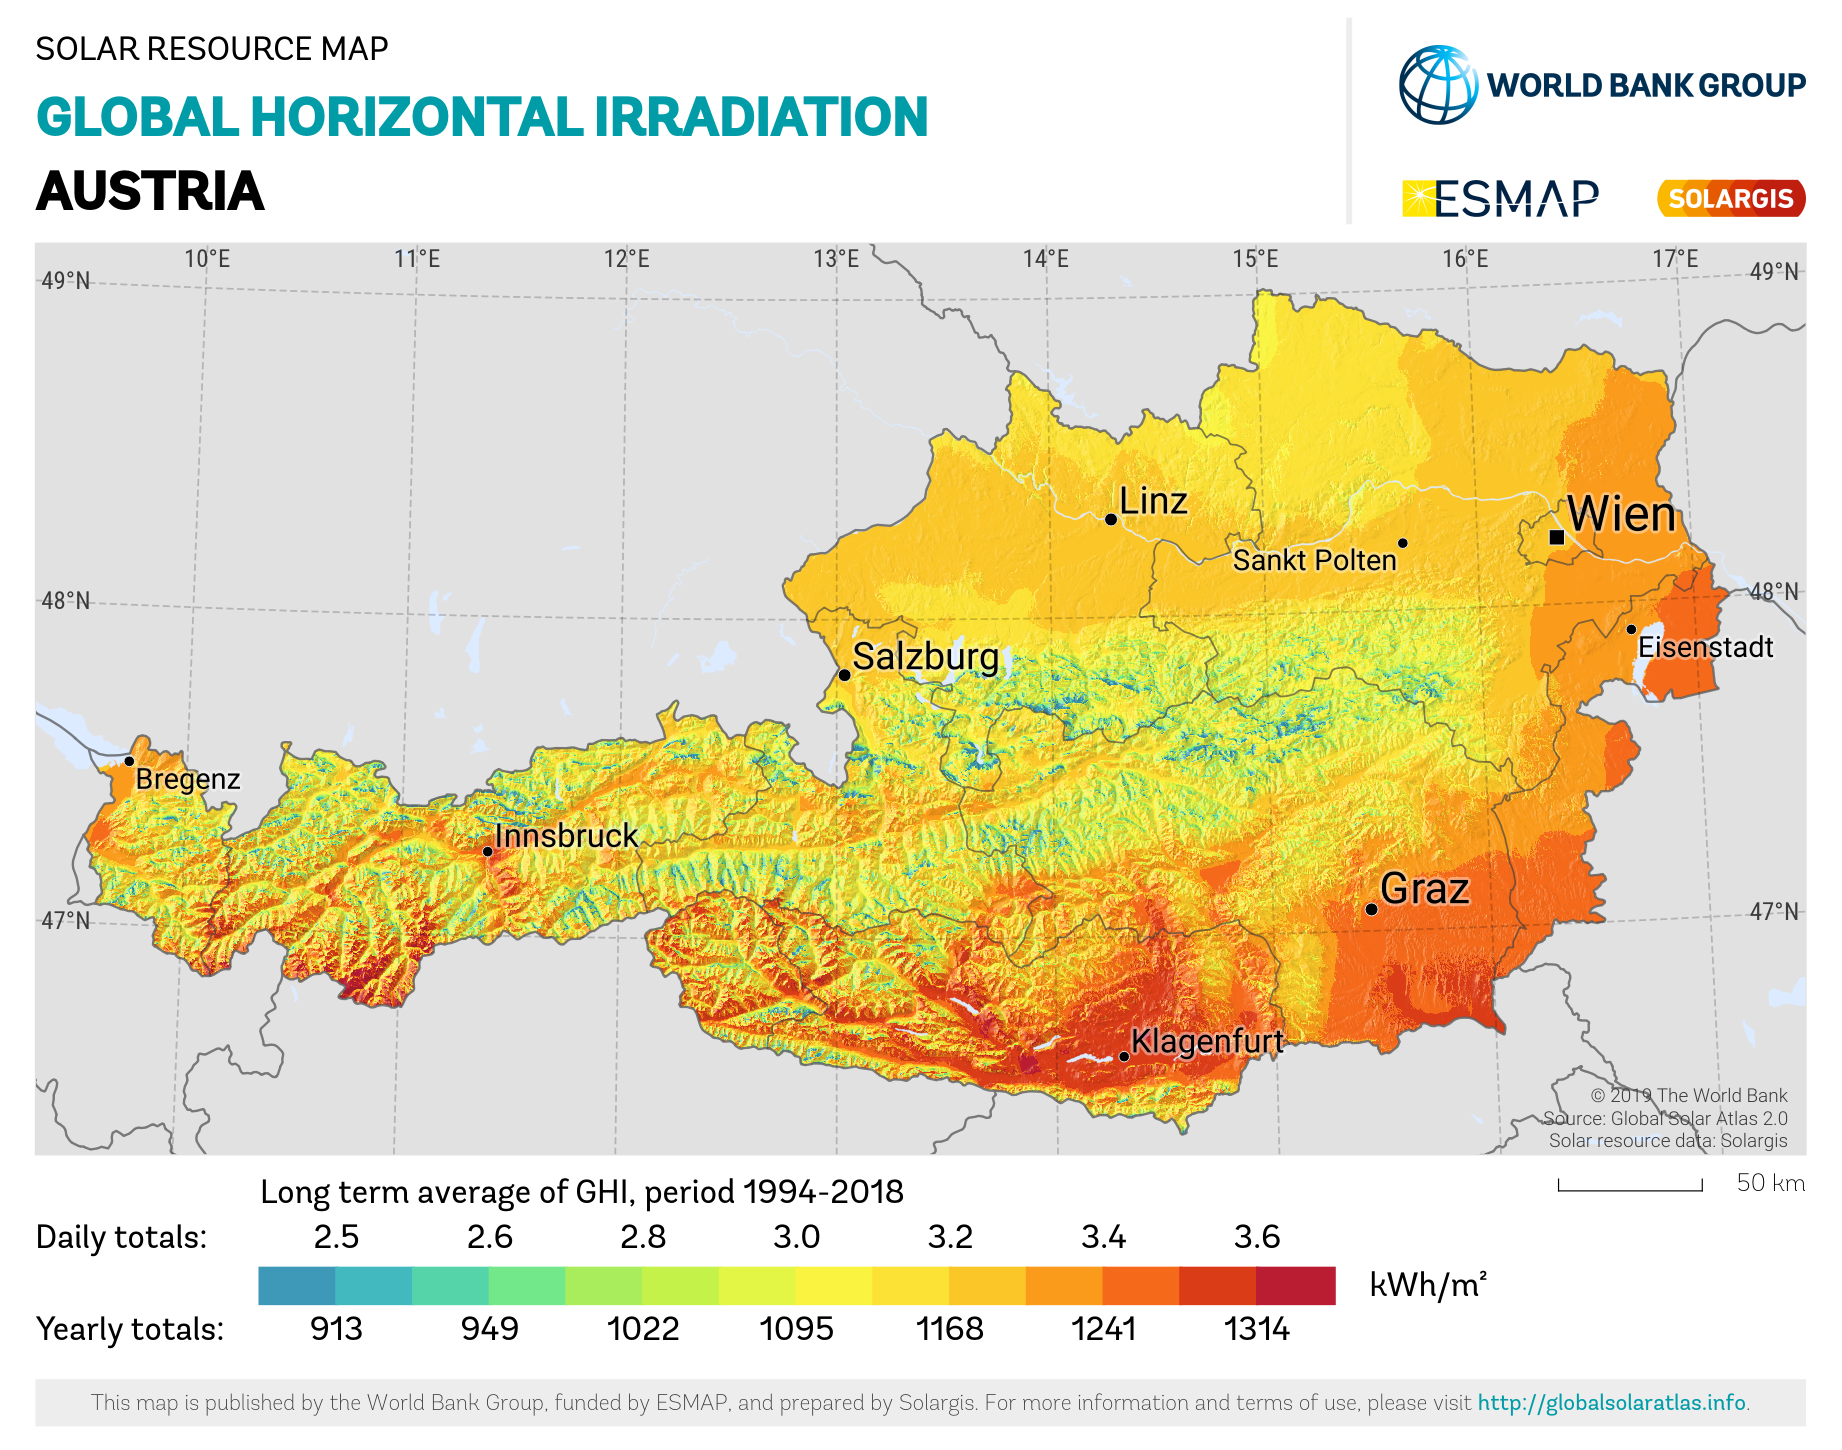
\includegraphics[width = 0.96\textwidth]{solar_maps/austria/austria_ghi}
  	\caption{Solar resource map of the long term average global horizontal irradiation of Austria. (Image credit: \cite{GlobalSolarAtlas:2020, Solargis:2021})}
	\label{fig:ghi_austria}
\end{figure}
\begin{figure}[h!]
	\centering
  	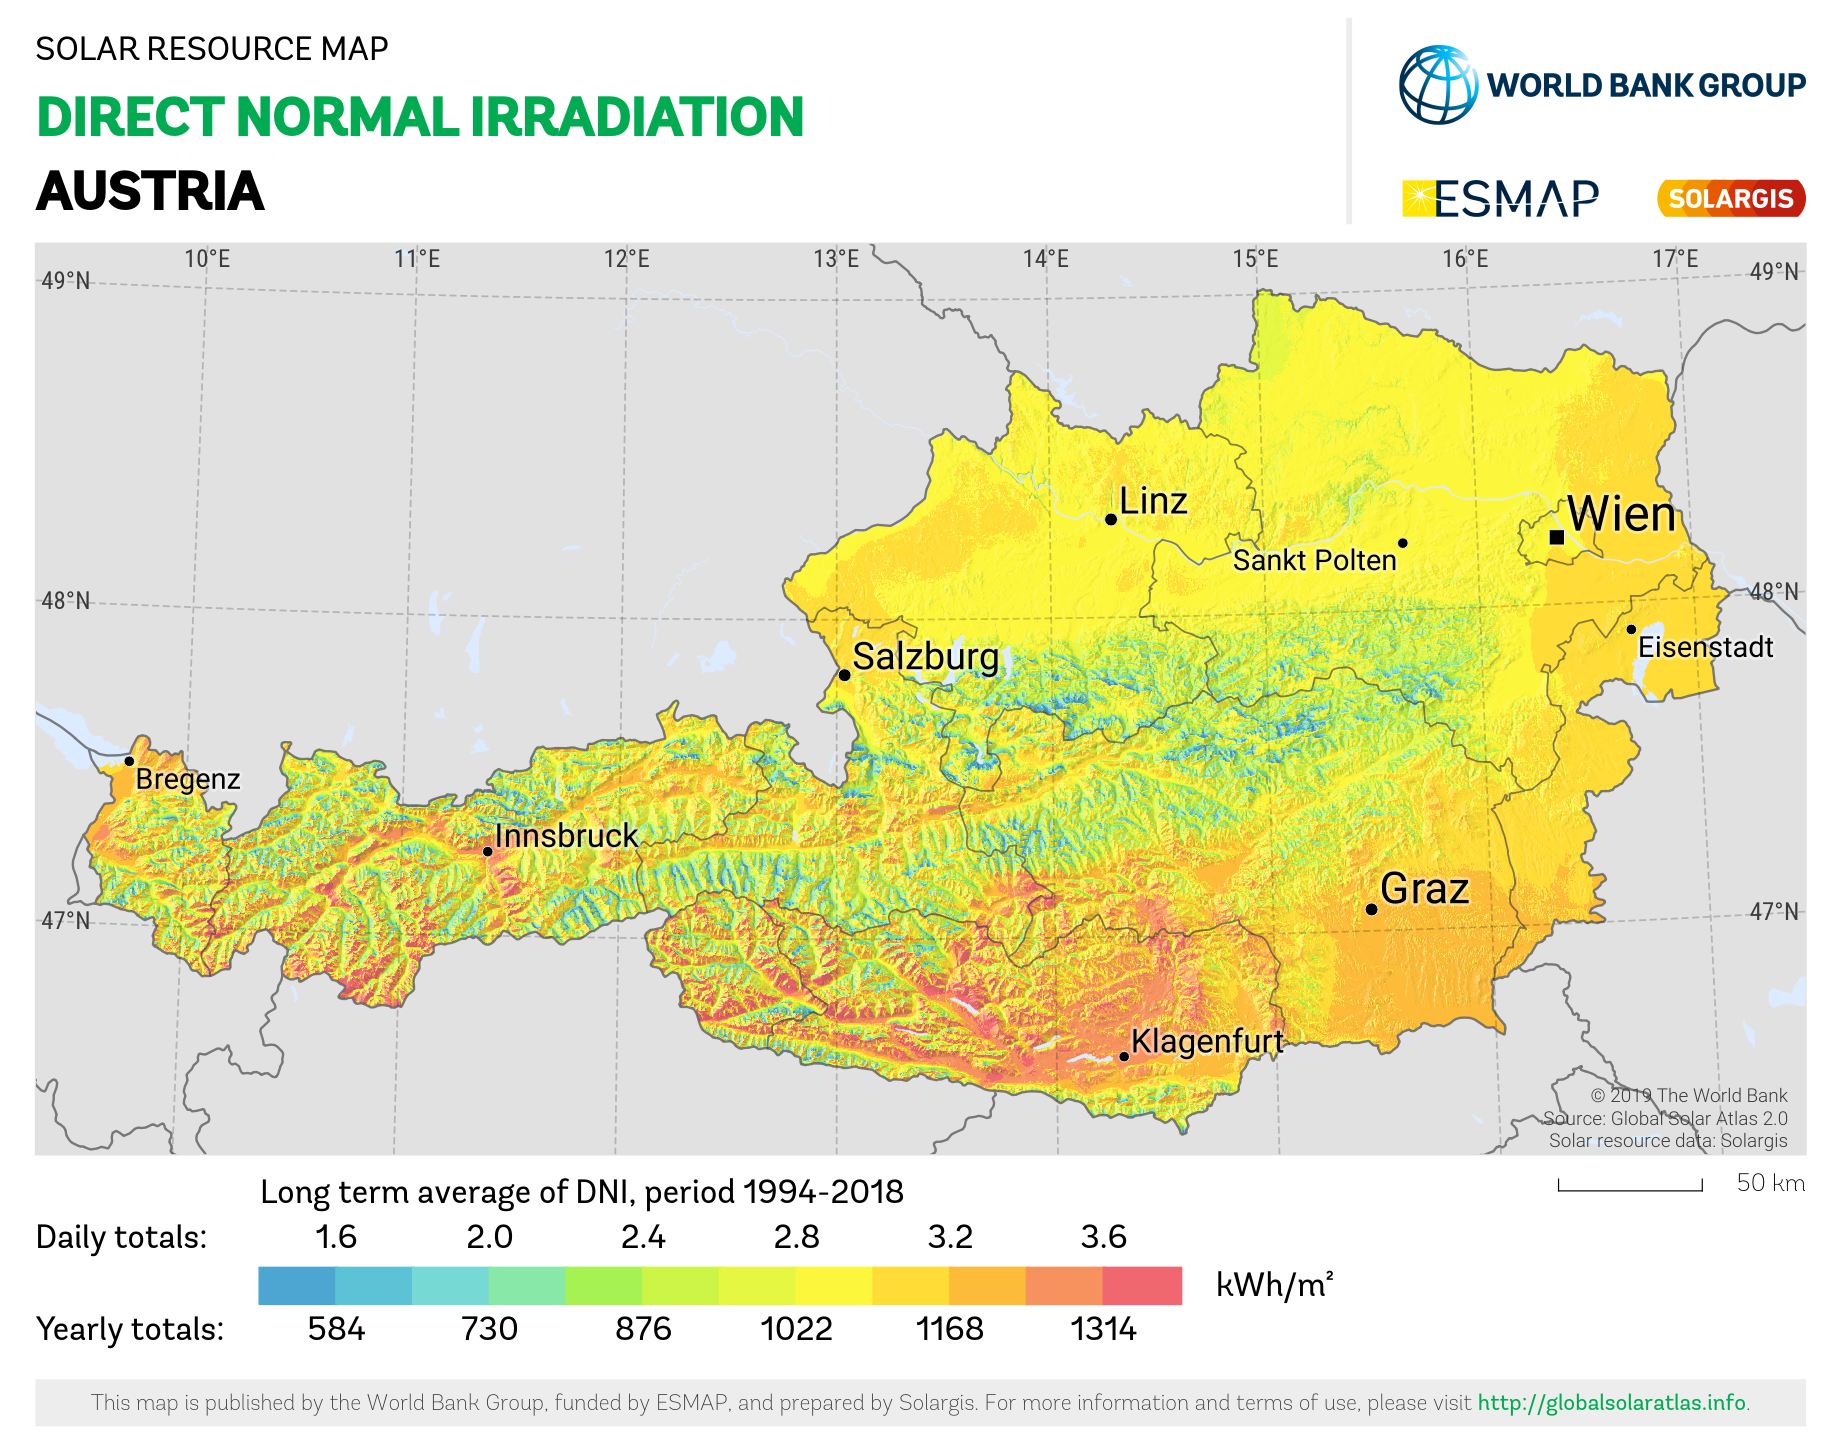
\includegraphics[width = 0.96\textwidth]{solar_maps/austria/austria_dni}
	\caption{Solar resource map of the long term average direct normal irradiation of Austria. (Image credit: \cite{GlobalSolarAtlas:2020, Solargis:2021})}
	\label{fig:dni_austria}
\end{figure}

It can be clearly seen that the values for both the global horizontal and the direct normal irradiation tend to be higher in the south and lower in the north of Austria. This can be partly explained by a greater latitude $\varphi$ which results in a lower altitude of the Sun $\gamma_{\mathrm{S}}$ during the winter months on the northern hemisphere ($\delta < 0$). Because of this, the Sun's incoming rays need to penetrate a thicker atmopshere and it is visible above the horizon for a shorter period of time over the course of the day. For locations in the south, such as the region around Klagenfurt, daily global horizontal irradiation totals of up to $3,50\mathrm{kWh}\mathrm{m}^{-2}$ and direct normal irradiation totals of up to $3,55\mathrm{kWh}\mathrm{m}^{-2}$ and higher can be expected, whereas loactions in the north, such as the region around Linz, only reach daily global horizontal irradiation totals of around $3,25\mathrm{kWh}\mathrm{m}^{-2}$ and daily direct normal irradiation totals of around $2,9\mathrm{kWh}\mathrm{m}^{-2}$. Another notable feature are valleys bordered by mountains in the south. In these valleys, and on the bounding north-facing mountain slopes, the daily global horizontal irradiation totals drop to less than $2,5\mathrm{kWh}\mathrm{m}^{-2}$ and the daily direct normal irradiation totals drop even further down to around $1,5\mathrm{kWh}\mathrm{m}^{-2}$. Examples for such valleys can be located all across the Alps and they highlight that locations with geographical features that block the direct path of the sunlight, should be discarded as installation sites for a PV generator \cite{Karttunen:2006, Mertens:2015, Wagner:2018}.

Using such maps, the \emph{global horizontal irradiance} (GHI) $E_{\mathrm{GHI}}$ in $\left( \mathrm{W}\mathrm{m}^{-2} \right)$ and the \emph{direct normal irradiance} (DNI) $E_{\mathrm{DNI}}$ in $\left( \mathrm{W}\mathrm{m}^{-2} \right)$ -- at a given location on Earth -- can be determined by dividing the values of the global horizontal and the direct normal irradiation by the time over which they were averaged. For instance by $24\mathrm{h}$ or by $365\mathrm{d} \cdot 24\mathrm{h}$ -- depending on which scale is used from the figures \ref{fig:ghi_austria} and \ref{fig:dni_austria} \cite{Mertens:2015, SolargisData:2020}.

The GHI is the sum of \emph{direct horizontal irradiance} (DHI) $E_{\mathrm{DHI}}$ in $\left( \mathrm{W}\mathrm{m}^{-2} \right)$ and the \emph{diffuse horizontal irradiance} (DIFH) $E_{\mathrm{DIFH}}$ in $\left( \mathrm{W} \mathrm{m}^{-2} \right)$ -- which is caused by the scattering of sunlight by Earth's atmosphere -- as shown in equation (\ref{eq:e_ghi}) \cite{Mertens:2015, SolarRadiationModeling:2020}.
	\begin{equation} \label{eq:e_ghi}
	\centering
		E_{\mathrm{GHI}} = E_{\mathrm{DHI}} + E_{\mathrm{DIFH}}
	\end{equation}

In comparison to the GHI -- which applies to a horizontal surface -- the DNI applies to a flat surface element perpendicular to the incoming Sun rays and it only consideres the direct irradiance \cite{Mertens:2015, SolarRadiationModeling:2020}. With simple trigonometry as shown in \cite{Mertens:2015}, the relationship between $E_{\mathrm{DNI}}$ and $E_{\mathrm{DHI}}$ can be written as:
	\begin{equation} \label{eq:e_dni}
	\centering
		E_{\mathrm{DNI}} = E_{\mathrm{DHI}} \, \frac{1}{\sin \gamma_{\mathrm{S}}} \text{.}
	\end{equation}

More precise solar resource maps for daily and monthly average global horizontal and direct normal irradiation are provided by \cite{Union:2020}.

\subsection{Photovoltaic energy yield} \label{sec:energy_yield}
As already mentioned in subsection \ref{sec:solar_irradiation_on_earths_surface} the decisive factors to determine the irradiance at a given location on the Earth's surface are the GHI and the DNI. Building on these, the three-component model as described in \cite{Landis:1995, Mertens:2015}, can be used to calculate the \emph{total irradiance} $E_{\mathrm{G}}$ in $\left( \mathrm{W}\mathrm{m}^{-2} \right)$ received by an inclined PV generator. The \emph{angle of inclination} with respect to the ground is $\beta$ in $\left( ^\circ \right)$. An example for such an inclined PV generator can be seen in the figures \ref{fig:tikz_three_component_model} and \ref{fig:tikz_angle_theta}.
\begin{figure}[h!]
	\centering
	

\tikzset{every picture/.style={line width=0.75pt}} %set default line width to 0.75pt        

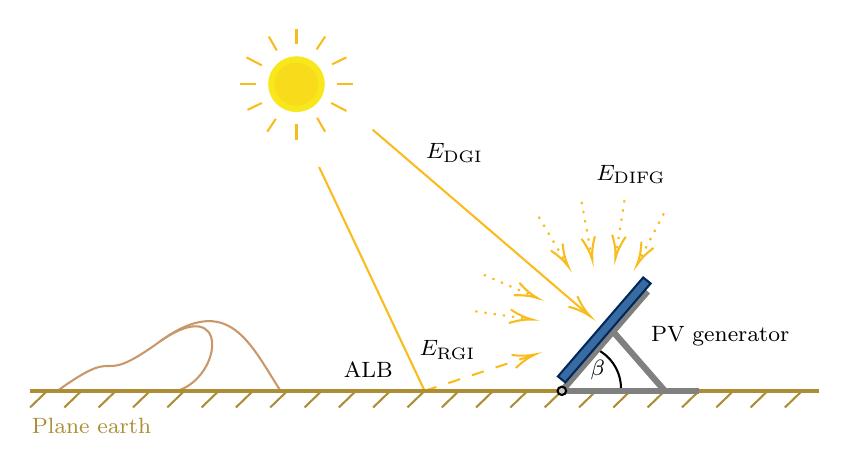
\begin{tikzpicture}[x=0.75pt,y=0.75pt,yscale=-1,xscale=1]
%uncomment if require: \path (0,468); %set diagram left start at 0, and has height of 468

%Straight Lines [id:da7639591375517361] 
\draw [color={rgb, 255:red, 248; green, 189; blue, 28 }  ,draw opacity=1 ]   (249.06,186.64) -- (299.9,294.48) ;
%Shape: Ellipse [id:dp07145193932966887] 
\draw  [color={rgb, 255:red, 248; green, 231; blue, 28 }  ,draw opacity=1 ][fill={rgb, 255:red, 248; green, 220; blue, 28 }  ,fill opacity=1 ][line width=2.25]  (226.02,146.71) .. controls (226.02,140.12) and (231.45,134.77) .. (238.15,134.77) .. controls (244.85,134.77) and (250.29,140.12) .. (250.29,146.71) .. controls (250.29,153.31) and (244.85,158.65) .. (238.15,158.65) .. controls (231.45,158.65) and (226.02,153.31) .. (226.02,146.71) -- cycle ;
%Curve Lines [id:da4839167804983171] 
\draw [color={rgb, 255:red, 202; green, 151; blue, 106 }  ,draw opacity=1 ]   (172.61,270.51) .. controls (206.08,247.35) and (202.78,287.29) .. (180.87,294.48) ;
%Curve Lines [id:da9367845814708875] 
\draw [color={rgb, 255:red, 202; green, 151; blue, 106 }  ,draw opacity=1 ]   (123.01,294.48) .. controls (156.08,270.51) and (139.55,294.48) .. (172.61,270.51) .. controls (205.67,246.55) and (216,272.11) .. (230.47,294.48) ;
%Straight Lines [id:da20208524763476388] 
\draw [color={rgb, 255:red, 248; green, 189; blue, 28 }  ,draw opacity=1 ] [dash pattern={on 4.5pt off 4.5pt}]  (299.9,294.48) -- (351.31,277.53) ;
\draw [shift={(353.21,276.9)}, rotate = 521.76] [color={rgb, 255:red, 248; green, 189; blue, 28 }  ,draw opacity=1 ][line width=0.75]    (10.93,-3.29) .. controls (6.95,-1.4) and (3.31,-0.3) .. (0,0) .. controls (3.31,0.3) and (6.95,1.4) .. (10.93,3.29)   ;
%Curve Lines [id:da8387867434601526] 
\draw    (382.96,274.51) .. controls (387.92,276.9) and (394.53,283.29) .. (394.53,293.68) ;
%Straight Lines [id:da056555134551903974] 
\draw [color={rgb, 255:red, 173; green, 142; blue, 55 }  ,draw opacity=1 ][fill={rgb, 255:red, 139; green, 87; blue, 42 }  ,fill opacity=1 ][line width=1.5]    (109.79,294.48) -- (490,294.48) ;
%Straight Lines [id:da48348316265398994] 
\draw [color={rgb, 255:red, 173; green, 142; blue, 55 }  ,draw opacity=1 ]   (134.59,294.48) -- (126.32,302.47) ;
%Straight Lines [id:da4565238298434817] 
\draw [color={rgb, 255:red, 173; green, 142; blue, 55 }  ,draw opacity=1 ]   (151.12,294.48) -- (142.85,302.47) ;
%Straight Lines [id:da7555358341240341] 
\draw [color={rgb, 255:red, 173; green, 142; blue, 55 }  ,draw opacity=1 ]   (167.65,294.48) -- (159.38,302.47) ;
%Straight Lines [id:da10247707612378121] 
\draw [color={rgb, 255:red, 173; green, 142; blue, 55 }  ,draw opacity=1 ]   (184.18,294.48) -- (175.91,302.47) ;
%Straight Lines [id:da22505664528789526] 
\draw [color={rgb, 255:red, 173; green, 142; blue, 55 }  ,draw opacity=1 ]   (200.71,294.48) -- (192.44,302.47) ;
%Straight Lines [id:da39883233893640213] 
\draw [color={rgb, 255:red, 173; green, 142; blue, 55 }  ,draw opacity=1 ]   (217.24,294.48) -- (208.98,302.47) ;
%Straight Lines [id:da9317267044471207] 
\draw [color={rgb, 255:red, 173; green, 142; blue, 55 }  ,draw opacity=1 ]   (233.77,294.48) -- (225.51,302.47) ;
%Straight Lines [id:da5689034971431022] 
\draw [color={rgb, 255:red, 173; green, 142; blue, 55 }  ,draw opacity=1 ]   (118.06,294.48) -- (109.79,302.47) ;
%Straight Lines [id:da6794614658982192] 
\draw [color={rgb, 255:red, 173; green, 142; blue, 55 }  ,draw opacity=1 ]   (250.3,294.48) -- (242.04,302.47) ;
%Straight Lines [id:da16884333894084147] 
\draw [color={rgb, 255:red, 173; green, 142; blue, 55 }  ,draw opacity=1 ]   (266.83,294.48) -- (258.57,302.47) ;
%Straight Lines [id:da5852948402158396] 
\draw [color={rgb, 255:red, 173; green, 142; blue, 55 }  ,draw opacity=1 ]   (283.36,294.48) -- (275.1,302.47) ;
%Straight Lines [id:da5569944189270981] 
\draw [color={rgb, 255:red, 173; green, 142; blue, 55 }  ,draw opacity=1 ]   (299.9,294.48) -- (291.63,302.47) ;
%Straight Lines [id:da07636127130608306] 
\draw [color={rgb, 255:red, 173; green, 142; blue, 55 }  ,draw opacity=1 ]   (316.43,294.48) -- (308.16,302.47) ;
%Straight Lines [id:da7270434905185723] 
\draw [color={rgb, 255:red, 173; green, 142; blue, 55 }  ,draw opacity=1 ]   (332.96,294.48) -- (324.69,302.47) ;
%Straight Lines [id:da5998901663023846] 
\draw [color={rgb, 255:red, 173; green, 142; blue, 55 }  ,draw opacity=1 ]   (349.49,294.48) -- (341.22,302.47) ;
%Straight Lines [id:da2586618910795322] 
\draw [color={rgb, 255:red, 173; green, 142; blue, 55 }  ,draw opacity=1 ]   (366.02,294.48) -- (357.75,302.47) ;
%Straight Lines [id:da2230405823513728] 
\draw [color={rgb, 255:red, 173; green, 142; blue, 55 }  ,draw opacity=1 ]   (382.55,294.48) -- (374.28,302.47) ;
%Straight Lines [id:da33268357962040995] 
\draw [color={rgb, 255:red, 173; green, 142; blue, 55 }  ,draw opacity=1 ]   (399.08,294.48) -- (390.81,302.47) ;
%Straight Lines [id:da9040529515577587] 
\draw [color={rgb, 255:red, 173; green, 142; blue, 55 }  ,draw opacity=1 ]   (415.61,294.48) -- (407.35,302.47) ;
%Straight Lines [id:da9864302443455792] 
\draw [color={rgb, 255:red, 173; green, 142; blue, 55 }  ,draw opacity=1 ]   (432.14,294.48) -- (423.88,302.47) ;
%Straight Lines [id:da5062470043832821] 
\draw [color={rgb, 255:red, 173; green, 142; blue, 55 }  ,draw opacity=1 ]   (448.67,294.48) -- (440.41,302.47) ;
%Straight Lines [id:da3838353864046502] 
\draw [color={rgb, 255:red, 173; green, 142; blue, 55 }  ,draw opacity=1 ]   (465.2,294.48) -- (456.94,302.47) ;
%Straight Lines [id:da7629428788396968] 
\draw [color={rgb, 255:red, 173; green, 142; blue, 55 }  ,draw opacity=1 ]   (481.73,294.48) -- (473.47,302.47) ;
%Straight Lines [id:da014514371361068923] 
\draw [color={rgb, 255:red, 128; green, 128; blue, 128 }  ,draw opacity=1 ][line width=2.25]    (407.35,246.55) -- (366.02,294.48) ;
%Straight Lines [id:da49954840219882635] 
\draw [color={rgb, 255:red, 128; green, 128; blue, 128 }  ,draw opacity=1 ][line width=2.25]    (432.14,294.48) -- (366.02,294.48) ;
%Straight Lines [id:da9965546684463125] 
\draw [color={rgb, 255:red, 128; green, 128; blue, 128 }  ,draw opacity=1 ][line width=2.25]    (391.23,266.52) -- (415.61,294.48) ;
%Straight Lines [id:da9786945806038319] 
\draw [color={rgb, 255:red, 248; green, 189; blue, 28 }  ,draw opacity=1 ] [dash pattern={on 0.84pt off 2.51pt}]  (415.2,209.01) -- (403.11,232) ;
\draw [shift={(402.18,233.77)}, rotate = 297.73] [color={rgb, 255:red, 248; green, 189; blue, 28 }  ,draw opacity=1 ][line width=0.75]    (10.93,-3.29) .. controls (6.95,-1.4) and (3.31,-0.3) .. (0,0) .. controls (3.31,0.3) and (6.95,1.4) .. (10.93,3.29)   ;
%Straight Lines [id:da4673310913126938] 
\draw [color={rgb, 255:red, 248; green, 189; blue, 28 }  ,draw opacity=1 ] [dash pattern={on 0.84pt off 2.51pt}]  (324.28,256.14) -- (349.78,259.84) ;
\draw [shift={(351.76,260.13)}, rotate = 188.27] [color={rgb, 255:red, 248; green, 189; blue, 28 }  ,draw opacity=1 ][line width=0.75]    (10.93,-3.29) .. controls (6.95,-1.4) and (3.31,-0.3) .. (0,0) .. controls (3.31,0.3) and (6.95,1.4) .. (10.93,3.29)   ;
%Straight Lines [id:da559627746158232] 
\draw [color={rgb, 255:red, 248; green, 189; blue, 28 }  ,draw opacity=1 ] [dash pattern={on 0.84pt off 2.51pt}]  (328.41,238.56) -- (352.4,248.95) ;
\draw [shift={(354.24,249.75)}, rotate = 203.41] [color={rgb, 255:red, 248; green, 189; blue, 28 }  ,draw opacity=1 ][line width=0.75]    (10.93,-3.29) .. controls (6.95,-1.4) and (3.31,-0.3) .. (0,0) .. controls (3.31,0.3) and (6.95,1.4) .. (10.93,3.29)   ;
%Straight Lines [id:da4533498063566359] 
\draw [color={rgb, 255:red, 248; green, 189; blue, 28 }  ,draw opacity=1 ] [dash pattern={on 0.84pt off 2.51pt}]  (375.52,203.42) -- (380.33,229.41) ;
\draw [shift={(380.69,231.37)}, rotate = 259.53] [color={rgb, 255:red, 248; green, 189; blue, 28 }  ,draw opacity=1 ][line width=0.75]    (10.93,-3.29) .. controls (6.95,-1.4) and (3.31,-0.3) .. (0,0) .. controls (3.31,0.3) and (6.95,1.4) .. (10.93,3.29)   ;
%Straight Lines [id:da995866694125163] 
\draw [color={rgb, 255:red, 248; green, 189; blue, 28 }  ,draw opacity=1 ] [dash pattern={on 0.84pt off 2.51pt}]  (396.19,202.62) -- (392.15,228.6) ;
\draw [shift={(391.85,230.57)}, rotate = 278.82] [color={rgb, 255:red, 248; green, 189; blue, 28 }  ,draw opacity=1 ][line width=0.75]    (10.93,-3.29) .. controls (6.95,-1.4) and (3.31,-0.3) .. (0,0) .. controls (3.31,0.3) and (6.95,1.4) .. (10.93,3.29)   ;
%Straight Lines [id:da13557132527331994] 
\draw [color={rgb, 255:red, 248; green, 189; blue, 28 }  ,draw opacity=1 ] [dash pattern={on 0.84pt off 2.51pt}]  (354.86,210.6) -- (368.1,232.85) ;
\draw [shift={(369.12,234.57)}, rotate = 239.25] [color={rgb, 255:red, 248; green, 189; blue, 28 }  ,draw opacity=1 ][line width=0.75]    (10.93,-3.29) .. controls (6.95,-1.4) and (3.31,-0.3) .. (0,0) .. controls (3.31,0.3) and (6.95,1.4) .. (10.93,3.29)   ;
%Shape: Ellipse [id:dp027496909576239847] 
\draw  [fill={rgb, 255:red, 202; green, 202; blue, 202 }  ,fill opacity=1 ] (363.95,294.48) .. controls (363.95,293.37) and (364.88,292.48) .. (366.02,292.48) .. controls (367.16,292.48) and (368.08,293.37) .. (368.08,294.48) .. controls (368.08,295.58) and (367.16,296.47) .. (366.02,296.47) .. controls (364.88,296.47) and (363.95,295.58) .. (363.95,294.48) -- cycle ;
%Straight Lines [id:da8059435922738829] 
\draw [color={rgb, 255:red, 248; green, 189; blue, 28 }  ,draw opacity=1 ]   (274.89,168.67) -- (378.14,257.23) ;
\draw [shift={(379.66,258.53)}, rotate = 220.62] [color={rgb, 255:red, 248; green, 189; blue, 28 }  ,draw opacity=1 ][line width=0.75]    (10.93,-3.29) .. controls (6.95,-1.4) and (3.31,-0.3) .. (0,0) .. controls (3.31,0.3) and (6.95,1.4) .. (10.93,3.29)   ;
%Straight Lines [id:da20746203736647328] 
\draw [color={rgb, 255:red, 248; green, 189; blue, 28 }  ,draw opacity=1 ]   (238.15,120) -- (238.15,127.43) ;
%Straight Lines [id:da7474001161810504] 
\draw [color={rgb, 255:red, 248; green, 189; blue, 28 }  ,draw opacity=1 ]   (265.3,146.71) -- (257.75,146.71) ;
%Straight Lines [id:da2676635751494898] 
\draw [color={rgb, 255:red, 248; green, 189; blue, 28 }  ,draw opacity=1 ]   (238.15,173.43) -- (238.15,165.99) ;
%Straight Lines [id:da5591085501687709] 
\draw [color={rgb, 255:red, 248; green, 189; blue, 28 }  ,draw opacity=1 ]   (218.55,146.71) -- (211,146.71) ;
%Straight Lines [id:da29943329422514986] 
\draw [color={rgb, 255:red, 248; green, 189; blue, 28 }  ,draw opacity=1 ]   (254.9,155.79) -- (262.18,159.61) ;
%Straight Lines [id:da8331061745611166] 
\draw [color={rgb, 255:red, 248; green, 189; blue, 28 }  ,draw opacity=1 ]   (214.12,133.82) -- (221.41,137.64) ;
%Straight Lines [id:da7334533162645056] 
\draw [color={rgb, 255:red, 248; green, 189; blue, 28 }  ,draw opacity=1 ]   (262.18,133.82) -- (255.32,137.16) ;
%Straight Lines [id:da16844895743023902] 
\draw [color={rgb, 255:red, 248; green, 189; blue, 28 }  ,draw opacity=1 ]   (221.41,155.79) -- (214.55,159.13) ;
%Straight Lines [id:da941363141001635] 
\draw [color={rgb, 255:red, 248; green, 189; blue, 28 }  ,draw opacity=1 ]   (247.86,129.97) -- (251.98,123.79) ;
%Straight Lines [id:da8944108780017783] 
\draw [color={rgb, 255:red, 248; green, 189; blue, 28 }  ,draw opacity=1 ]   (224.07,169.61) -- (228.2,163.43) ;
%Straight Lines [id:da6072002125224827] 
\draw [color={rgb, 255:red, 248; green, 189; blue, 28 }  ,draw opacity=1 ]   (248.1,162.95) -- (251.98,169.64) ;
%Straight Lines [id:da7935478336524533] 
\draw [color={rgb, 255:red, 248; green, 189; blue, 28 }  ,draw opacity=1 ]   (224.8,123.79) -- (228.69,130.48) ;
%Shape: Rectangle [id:dp22359865545582847] 
\draw  [color={rgb, 255:red, 0; green, 41; blue, 90 }  ,draw opacity=1 ][fill={rgb, 255:red, 57; green, 107; blue, 163 }  ,fill opacity=1 ] (408.78,242.74) -- (367.69,290.39) -- (364.12,287.51) -- (405.21,239.86) -- cycle ;

% Text Node
\draw (378.38,278.09) node [anchor=north west][inner sep=0.75pt]  [font=\footnotesize]  {$\beta $};
% Text Node
\draw (109.15,306.05) node [anchor=north west][inner sep=0.75pt]  [font=\footnotesize,color={rgb, 255:red, 173; green, 142; blue, 55 }  ,opacity=1 ] [align=left] {Plane earth};
% Text Node
\draw (299.12,173.75) node [anchor=north west][inner sep=0.75pt]  [font=\footnotesize]  {$E_{\mathrm{DGI}}$};
% Text Node
\draw (407.48,262.12) node [anchor=north west][inner sep=0.75pt]  [font=\footnotesize] [align=left] {PV generator};
% Text Node
\draw (381.17,184.14) node [anchor=north west][inner sep=0.75pt]  [font=\footnotesize]  {$E_{\mathrm{DIFG}}$};
% Text Node
\draw (295.99,268.8) node [anchor=north west][inner sep=0.75pt]  [font=\footnotesize]  {$E_{\mathrm{RGI}}$};
% Text Node
\draw (259.45,279.09) node [anchor=north west][inner sep=0.75pt]  [font=\footnotesize]  {$\mathrm{ALB}$};


\end{tikzpicture}

	\caption{Solar radiation on an inclined photovoltaic generator with the angle $\beta$. (Recreated from: \cite{Mertens:2015})}
	\label{fig:tikz_three_component_model}
\end{figure}
Figure \ref{fig:tikz_three_component_model} illustrates that the total irradiance received by an inlcined PV generator is made up of the sum of the \emph{direct generator irradiance} (DGI) $E_{\mathrm{DGI}}$ in $\left( \mathrm{W}\mathrm{m}^{-2} \right)$, the \emph{diffuse generator irradiance} (DIFG) $E_{\mathrm{DIFG}}$ in $\left( \mathrm{W}\mathrm{m}^{-2} \right)$ and the \emph{reflected generator irradiance} (RGI) $E_{\mathrm{RGI}}$ in $\left( \mathrm{W}\mathrm{m}^{-2} \right)$. The latter is reflected with an \emph{albedo value} $\mathrm{ALB}$ in $\left( 1 \right)$ from plane earth onto the PV generator. This relationship can be written as follows \cite{Bennett:2010, Bertol:2011, Mertens:2015, Bralower:2018}:
	\begin{equation} \label{eq:e_gen}
	\centering
		E_{\mathrm{G}} = E_{\mathrm{DGI}} + E_{\mathrm{DIFG}} + E_{\mathrm{RGI}}
	\end{equation}

The first component from equation (\ref{eq:e_gen}) can be determined by considering the \emph{angle of incidence} $\theta$ of the solar rays in $\left( ^\circ \right)$ with respect to the normal of the PV generator's energy-converting area $A_{\mathrm{PV}}$, as presented in equation (\ref{eq:e_dgi}). Figure \ref{fig:tikz_angle_theta} provides an illustration of the angle $\theta$ for which the cosine can be obtained from equation (\ref{eq:cos_theta}).
	\begin{equation} \label{eq:e_dgi}
	\centering
		E_{\mathrm{DGI}} = E_{\mathrm{DNI}} \, \cos \theta
	\end{equation}
	\begin{equation} \label{eq:cos_theta}
	\centering
		\begin{aligned}
		\cos \theta &= \sin \delta \, \sin \varphi \, \cos \beta - \sin \delta \, \cos \varphi \, \sin \beta \, \cos \alpha_{\mathrm{S}}(t_\mathrm{S} = 12\mathrm{h}) \\
		&+ \cos \delta \, \cos \varphi \, \cos \beta \, \cos h_{\mathrm{S}} + \cos \delta \, \sin \varphi \, \sin \beta \, \cos \alpha_{\mathrm{S}} \, \cos h_{\mathrm{S}} \\ &+ \cos \delta \, \sin \beta \, \cos h_{\mathrm{S}} \, \sin \alpha_{\mathrm{S}}(t_\mathrm{S} = 12\mathrm{h})
		\end{aligned}
	\end{equation}
\begin{figure}[h!]
	\centering
	

\tikzset{every picture/.style={line width=0.75pt}} %set default line width to 0.75pt        

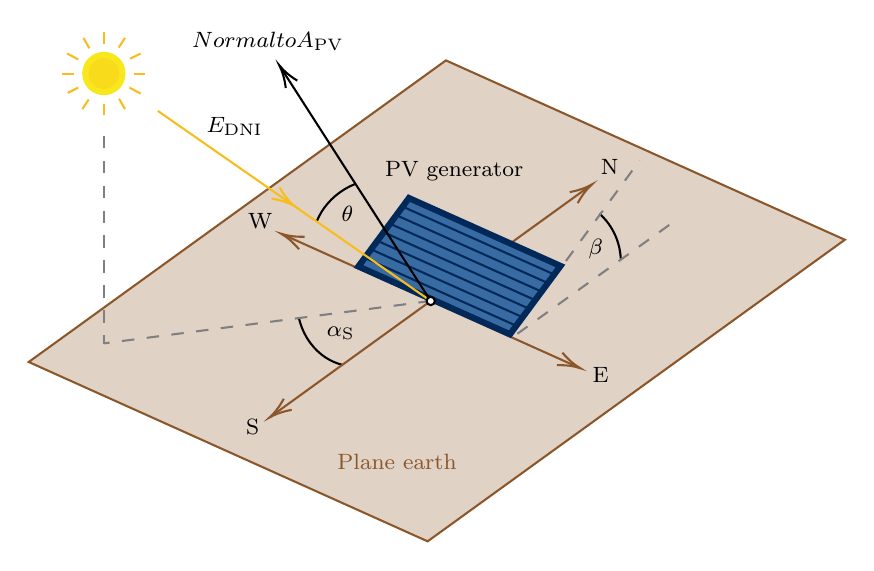
\begin{tikzpicture}[x=0.75pt,y=0.75pt,yscale=-1,xscale=1]
%uncomment if require: \path (0,455); %set diagram left start at 0, and has height of 455

%Shape: Rectangle [id:dp8474155302282593] 
\draw  [color={rgb, 255:red, 139; green, 87; blue, 42 }  ,draw opacity=1 ][fill={rgb, 255:red, 139; green, 87; blue, 42 }  ,fill opacity=0.27 ] (304.8,113.67) -- (496.99,200.08) -- (295.98,345.38) -- (103.79,258.97) -- cycle ;
%Straight Lines [id:da6680786992692076] 
\draw [color={rgb, 255:red, 139; green, 87; blue, 42 }  ,draw opacity=1 ]   (367.73,261.16) -- (227.22,197.98) ;
\draw [shift={(225.39,197.16)}, rotate = 384.21000000000004] [color={rgb, 255:red, 139; green, 87; blue, 42 }  ,draw opacity=1 ][line width=0.75]    (10.93,-3.29) .. controls (6.95,-1.4) and (3.31,-0.3) .. (0,0) .. controls (3.31,0.3) and (6.95,1.4) .. (10.93,3.29)   ;
\draw [shift={(369.56,261.98)}, rotate = 204.21] [color={rgb, 255:red, 139; green, 87; blue, 42 }  ,draw opacity=1 ][line width=0.75]    (10.93,-3.29) .. controls (6.95,-1.4) and (3.31,-0.3) .. (0,0) .. controls (3.31,0.3) and (6.95,1.4) .. (10.93,3.29)   ;
%Shape: Arc [id:dp4091032640411232] 
\draw  [draw opacity=0] (378.78,187.54) .. controls (381.04,189.51) and (383.04,191.89) .. (384.69,194.67) .. controls (387.37,199.17) and (388.78,204.17) .. (389.04,209.19) -- (360,211.71) -- cycle ; \draw   (378.78,187.54) .. controls (381.04,189.51) and (383.04,191.89) .. (384.69,194.67) .. controls (387.37,199.17) and (388.78,204.17) .. (389.04,209.19) ;
%Shape: Ellipse [id:dp7766653682919293] 
\draw  [color={rgb, 255:red, 248; green, 231; blue, 28 }  ,draw opacity=1 ][fill={rgb, 255:red, 248; green, 220; blue, 28 }  ,fill opacity=1 ][line width=2.25]  (131.06,120) .. controls (131.06,115.06) and (135.06,111.06) .. (140,111.06) .. controls (144.94,111.06) and (148.94,115.06) .. (148.94,120) .. controls (148.94,124.94) and (144.94,128.94) .. (140,128.94) .. controls (135.06,128.94) and (131.06,124.94) .. (131.06,120) -- cycle ;
%Straight Lines [id:da12322467795106329] 
\draw [color={rgb, 255:red, 248; green, 189; blue, 28 }  ,draw opacity=1 ]   (140,100) -- (140,105.56) ;
%Straight Lines [id:da4332784077616083] 
\draw [color={rgb, 255:red, 248; green, 189; blue, 28 }  ,draw opacity=1 ]   (160,120) -- (154.44,120) ;
%Straight Lines [id:da7027066659727501] 
\draw [color={rgb, 255:red, 248; green, 189; blue, 28 }  ,draw opacity=1 ]   (140,140) -- (140,134.44) ;
%Straight Lines [id:da11414191136971219] 
\draw [color={rgb, 255:red, 248; green, 189; blue, 28 }  ,draw opacity=1 ]   (125.56,120) -- (120,120) ;
%Straight Lines [id:da6688063172227983] 
\draw [color={rgb, 255:red, 248; green, 189; blue, 28 }  ,draw opacity=1 ]   (152.34,126.79) -- (157.7,129.65) ;
%Straight Lines [id:da20949775152165007] 
\draw [color={rgb, 255:red, 248; green, 189; blue, 28 }  ,draw opacity=1 ]   (122.3,110.35) -- (127.66,113.21) ;
%Straight Lines [id:da7656758253367213] 
\draw [color={rgb, 255:red, 248; green, 189; blue, 28 }  ,draw opacity=1 ]   (157.7,110.35) -- (152.65,112.85) ;
%Straight Lines [id:da9791803411373596] 
\draw [color={rgb, 255:red, 248; green, 189; blue, 28 }  ,draw opacity=1 ]   (127.66,126.79) -- (122.61,129.3) ;
%Straight Lines [id:da2234053647148624] 
\draw [color={rgb, 255:red, 248; green, 189; blue, 28 }  ,draw opacity=1 ]   (147.15,107.46) -- (150.19,102.84) ;
%Straight Lines [id:da6726326270351066] 
\draw [color={rgb, 255:red, 248; green, 189; blue, 28 }  ,draw opacity=1 ]   (129.63,137.14) -- (132.67,132.51) ;
%Straight Lines [id:da7766925486897012] 
\draw [color={rgb, 255:red, 248; green, 189; blue, 28 }  ,draw opacity=1 ]   (147.33,132.16) -- (150.19,137.16) ;
%Straight Lines [id:da3318298152117709] 
\draw [color={rgb, 255:red, 248; green, 189; blue, 28 }  ,draw opacity=1 ]   (130.17,102.84) -- (133.03,107.84) ;

%Straight Lines [id:da4654469204608218] 
\draw [color={rgb, 255:red, 128; green, 128; blue, 128 }  ,draw opacity=1 ] [dash pattern={on 4.5pt off 4.5pt}]  (140,150) -- (140,250.5) ;
%Shape: Arc [id:dp19974251160210033] 
\draw  [draw opacity=0] (255.22,260.43) .. controls (249.27,259.03) and (243.7,255.49) .. (239.53,249.88) .. controls (236.81,246.23) and (234.96,242.08) .. (233.96,237.75) -- (261.41,229.35) -- cycle ; \draw   (255.22,260.43) .. controls (249.27,259.03) and (243.7,255.49) .. (239.53,249.88) .. controls (236.81,246.23) and (234.96,242.08) .. (233.96,237.75) ;
%Straight Lines [id:da5130479264192895] 
\draw [color={rgb, 255:red, 139; green, 87; blue, 42 }  ,draw opacity=1 ]   (373.59,174.56) -- (221.36,284.59) ;
\draw [shift={(219.74,285.76)}, rotate = 324.14] [color={rgb, 255:red, 139; green, 87; blue, 42 }  ,draw opacity=1 ][line width=0.75]    (10.93,-3.29) .. controls (6.95,-1.4) and (3.31,-0.3) .. (0,0) .. controls (3.31,0.3) and (6.95,1.4) .. (10.93,3.29)   ;
\draw [shift={(375.21,173.38)}, rotate = 144.14] [color={rgb, 255:red, 139; green, 87; blue, 42 }  ,draw opacity=1 ][line width=0.75]    (10.93,-3.29) .. controls (6.95,-1.4) and (3.31,-0.3) .. (0,0) .. controls (3.31,0.3) and (6.95,1.4) .. (10.93,3.29)   ;
%Straight Lines [id:da7333561757823057] 
\draw [color={rgb, 255:red, 128; green, 128; blue, 128 }  ,draw opacity=1 ] [dash pattern={on 4.5pt off 4.5pt}]  (297.47,229.57) -- (140,250) ;
%Shape: Rectangle [id:dp9181904913709493] 
\draw  [color={rgb, 255:red, 0; green, 41; blue, 90 }  ,draw opacity=1 ][fill={rgb, 255:red, 57; green, 107; blue, 163 }  ,fill opacity=1 ][line width=2.25]  (286.99,180) -- (360,212.71) -- (335.66,245.63) -- (262.65,212.93) -- cycle ;
%Straight Lines [id:da13478383057933563] 
\draw [color={rgb, 255:red, 0; green, 41; blue, 90 }  ,draw opacity=1 ]   (283.95,184.12) -- (356.96,216.82) ;
%Straight Lines [id:da5884374823291068] 
\draw [color={rgb, 255:red, 0; green, 41; blue, 90 }  ,draw opacity=1 ]   (265.69,208.81) -- (338.7,241.52) ;
%Straight Lines [id:da02285619917411874] 
\draw [color={rgb, 255:red, 0; green, 41; blue, 90 }  ,draw opacity=1 ]   (268.74,204.7) -- (341.75,237.4) ;
%Straight Lines [id:da23820193833800274] 
\draw [color={rgb, 255:red, 0; green, 41; blue, 90 }  ,draw opacity=1 ]   (271.78,200.58) -- (344.79,233.28) ;
%Straight Lines [id:da14178706586084355] 
\draw [color={rgb, 255:red, 0; green, 41; blue, 90 }  ,draw opacity=1 ]   (280.9,188.23) -- (353.91,220.94) ;
%Straight Lines [id:da14421525428340431] 
\draw [color={rgb, 255:red, 0; green, 41; blue, 90 }  ,draw opacity=1 ]   (274.82,196.46) -- (347.83,229.17) ;
%Straight Lines [id:da3643942316695261] 
\draw [color={rgb, 255:red, 0; green, 41; blue, 90 }  ,draw opacity=1 ]   (277.86,192.35) -- (350.87,225.05) ;
%Shape: Arc [id:dp7190646059564607] 
\draw  [draw opacity=0] (242.59,191.14) .. controls (245.03,185.16) and (249.56,179.68) .. (255.82,175.84) .. controls (257.47,174.83) and (259.17,173.97) .. (260.9,173.27) -- (269.51,198.17) -- cycle ; \draw   (242.59,191.14) .. controls (245.03,185.16) and (249.56,179.68) .. (255.82,175.84) .. controls (257.47,174.83) and (259.17,173.97) .. (260.9,173.27) ;
%Straight Lines [id:da4133530859205612] 
\draw [color={rgb, 255:red, 248; green, 189; blue, 28 }  ,draw opacity=1 ][line width=0.75]    (166,138) -- (230.1,182.64) ;
\draw [shift={(231.74,183.79)}, rotate = 214.86] [color={rgb, 255:red, 248; green, 189; blue, 28 }  ,draw opacity=1 ][line width=0.75]    (10.93,-3.29) .. controls (6.95,-1.4) and (3.31,-0.3) .. (0,0) .. controls (3.31,0.3) and (6.95,1.4) .. (10.93,3.29)   ;
%Straight Lines [id:da8270043512595768] 
\draw [color={rgb, 255:red, 248; green, 189; blue, 28 }  ,draw opacity=1 ][line width=0.75]    (231.74,183.79) -- (297.47,229.57) ;
%Straight Lines [id:da7037472432355609] 
\draw [color={rgb, 255:red, 0; green, 0; blue, 0 }  ,draw opacity=1 ]   (297.47,229.57) -- (225.58,117.68) ;
\draw [shift={(224.5,116)}, rotate = 417.28] [color={rgb, 255:red, 0; green, 0; blue, 0 }  ,draw opacity=1 ][line width=0.75]    (10.93,-3.29) .. controls (6.95,-1.4) and (3.31,-0.3) .. (0,0) .. controls (3.31,0.3) and (6.95,1.4) .. (10.93,3.29)   ;
%Straight Lines [id:da7634900279620906] 
\draw [color={rgb, 255:red, 128; green, 128; blue, 128 }  ,draw opacity=1 ] [dash pattern={on 4.5pt off 4.5pt}]  (412.4,192.95) -- (334.66,248.63) ;
%Straight Lines [id:da3198763131888107] 
\draw [color={rgb, 255:red, 128; green, 128; blue, 128 }  ,draw opacity=1 ] [dash pattern={on 4.5pt off 4.5pt}]  (362.64,210.28) -- (398.15,161.88) ;
%Shape: Circle [id:dp009625788709507033] 
\draw  [fill={rgb, 255:red, 255; green, 255; blue, 255 }  ,fill opacity=1 ] (295.47,229.57) .. controls (295.47,228.47) and (296.37,227.57) .. (297.47,227.57) .. controls (298.58,227.57) and (299.47,228.47) .. (299.47,229.57) .. controls (299.47,230.68) and (298.58,231.57) .. (297.47,231.57) .. controls (296.37,231.57) and (295.47,230.68) .. (295.47,229.57) -- cycle ;

% Text Node
\draw (372,198.4) node [anchor=north west][inner sep=0.75pt]  [font=\footnotesize]  {$\beta $};
% Text Node
\draw (378,160) node [anchor=north west][inner sep=0.75pt]  [font=\footnotesize] [align=left] {N};
% Text Node
\draw (207,285) node [anchor=north west][inner sep=0.75pt]  [font=\footnotesize] [align=left] {S};
% Text Node
\draw (374,260) node [anchor=north west][inner sep=0.75pt]  [font=\footnotesize] [align=left] {E};
% Text Node
\draw (208,186) node [anchor=north west][inner sep=0.75pt]  [font=\footnotesize] [align=left] {W};
% Text Node
\draw (274,161) node [anchor=north west][inner sep=0.75pt]  [font=\footnotesize] [align=left] {PV generator};
% Text Node
\draw (246,240.4) node [anchor=north west][inner sep=0.75pt]  [font=\footnotesize]  {$\alpha _{\mathrm{S}}$};
% Text Node
\draw (253,182.4) node [anchor=north west][inner sep=0.75pt]  [font=\footnotesize]  {$\theta $};
% Text Node
\draw (251,302) node [anchor=north west][inner sep=0.75pt]  [font=\footnotesize,color={rgb, 255:red, 139; green, 87; blue, 42 }  ,opacity=1 ] [align=left] {Plane earth};
% Text Node
\draw (188,139.4) node [anchor=north west][inner sep=0.75pt]  [font=\footnotesize]  {$E_{\mathrm{DNI}}$};
% Text Node
\draw (181,98.4) node [anchor=north west][inner sep=0.75pt]  [font=\footnotesize]  {$\text{Normal to } A_{\mathrm{PV}}$};


\end{tikzpicture}

	\caption{Illustration of the incidence angle $\theta$ of the solar rays with respect to the normal to $A_\mathrm{PV}$. (Recreated from: \cite{Landis:1995})}
	\label{fig:tikz_angle_theta}
\end{figure}
The angle of incidence $\theta$ has a range of $\left[0^\circ \text{, } 90^\circ\right]$ and $\alpha_\mathrm{S}(t_\mathrm{S} = 12\mathrm{h})$ represents the orientation of the normal to $A_\mathrm{PV}$. For completenes it must be mentioned that equation (\ref{eq:sin_gamma_s}) can be derived from equation (\ref{eq:cos_theta}) with $\beta = 0^\circ$, and that in the case $\gamma_{\mathrm{S}} + \beta = 90^\circ$, the Sun's rays are perpendicular to the PV generator's energy-converting area $A_{\mathrm{PV}}$ which results in $E_{\mathrm{DGI}} = E_{\mathrm{DNI}}$ \cite{Landis:1995, Bertol:2011, Mertens:2015, Wagner:2018}.

To determine the second component from equation (\ref{eq:e_gen}) the sky is assumed to be isotropic. This means that the DIFH is evenly distributed in the entire celestial hemisphere above the PV generator. The more the PV generator is inclined the smaller the proportion of DIFG in equation (\ref{eq:e_difg}) becomes (compare to figure \ref{fig:tikz_three_component_model}) \cite{Landis:1995, Mertens:2015}. 
	\begin{equation} \label{eq:e_difg}
	\centering
		E_{\mathrm{DIFG}} = E_{\mathrm{DIFH}} \, \frac{1 + \cos \beta }{2}
	\end{equation} 
In the book \cite{Mertens:2015} it is expressly pointed out that the isotropic approach used in equation (\ref{eq:e_difg}) is only a rough approximation. This is because the sky is brighter towards the Sun than towards the horizon.\footnote{More precise equations would be difficult to derive, which would go beyond the scope of this thesis.} 

When examining the last component from equation (\ref{eq:e_gen}) it has to be taken into account that different surfaces -- on which a PV generator is placed -- reflect solar rays differently. In equation (\ref{eq:e_rgi}) this is accomplished with the factor $\mathrm{ALB}$ -- also known as the reflectivity. Similar to equation (\ref{eq:e_difg}) an isotropic approach is used \cite{Landis:1995, Dobos:2011, Mertens:2015, Bralower:2018}. 
	\begin{equation} \label{eq:e_rgi}
	\centering
		E_{\mathrm{RGI}} = E_{\mathrm{GHI}} \, \frac{1 - \cos \beta }{2} \cdot \mathrm{ALB}
	\end{equation}
Approximate albedo values for various surfaces are listed in table \ref{tab:table_albedo}. The larger the value the more solar rays are reflected. A blackbody for example has an albedo value of 0 while an absolute white surface has an albedo value of 1. The Earth has an average albedo of 0,31 \cite{Bennett:2010, Dobos:2011, Bralower:2018}.
\begin{table}[h!]
	\centering
	\footnotesize
\begin{tabular}{|l|c|l|c|}
	\hline
	\textbf{Surface} & \textbf{Albedo} & \textbf{Surface} & \textbf{Albedo} \\
	\hline
	Forest & 0,05 -- 0,18 & Sand & 0,20 -- 0,40 \\
	Water & 0,06 -- 0,10 & Grass (July, August) & 0,25 \\
	Rain forest & 0,07 -- 0,15 & Dry sandy soil & 0,25 -- 0,45 \\
	Coniferous forest & 0,09 -- 0,15 & Uncultivated field & 0,26 \\
	Dark-colored soil surfaces & 0,10 -- 0,20 & New concrete & 0,30 \\
	Heathland & 0,10 -- 0,25 & Granite & 0,30 -- 0,35 \\
	Asphalt & 0,15 & Glacial ice & 0,30 -- 0,40 \\
	Deciduous forest & 0,15 -- 0,18 & Light-colored soil surfaces & 0,40 -- 0,50 \\
	Dry clay soil & 0,15 -- 0,35 & Old snow & 0,45 -- 0,70 \\
	Lawn & 0,18 -- 0,23 & Dry salt cover & 0,50 \\
	Weathered concrete & 0,20 & Fresh snow & 0,80 -- 0,90 \\
	\hline
\end{tabular}
	\caption{Albedo values (refelctivity) for different surfaces \cite{Dobos:2011, Bertol:2011, Mertens:2015, Bralower:2018}.}
	\label{tab:table_albedo}
\end{table}

If the three derived components $E_{\mathrm{DGI}}$, $E_{\mathrm{DIFG}}$ and $E_{\mathrm{RGI}}$ are now inserted into equation (\ref{eq:e_gen}) while considering the equations (\ref{eq:e_ghi}) and (\ref{eq:e_dni}), the total irradiance $E_{\mathrm{G}}$ received by an inclined PV generator, depending on $E_{\mathrm{GHI}}$, $E_{\mathrm{DNI}}$, $\gamma_{\mathrm{S}}$, $\beta$ and $\mathrm{ALB}$, can be obtained:
	\begin{equation} \label{eq:e_gen_ghi_dni}
	\centering
		\begin{split}
		E_{\mathrm{G}} = E_{\mathrm{DNI}} \, \cos \theta + \left(E_{\mathrm{GHI}} - E_{\mathrm{DNI}} \, \sin \gamma_{\mathrm{S}}\right) \frac{1 + \cos \beta }{2} \\ 
		+ E_{\mathrm{GHI}} \, \frac{1 - \cos \beta }{2} \cdot \mathrm{ALB} \text{.}
		\end{split}
	\end{equation}
Regarding this equation it must be noted that the angles $\gamma_{\mathrm{S}}$ and $\theta$ are time dependent and therefore $E_{\mathrm{G}}$ as well. $E_{\mathrm{GHI}}$ and $E_{\mathrm{DNI}}$ on the other hand are average values -- if taken from solar resource maps -- and can therefore be treated as constants. The angle of inclination $\beta$ as well as the albedo value $\mathrm{ALB}$ are also treated as constants. Once the PV generator is installed its inclination angle $\beta$ will not change for the entire duration of the mission. This has the consequence that the PV generator's inclined energy-converting area $A_{\mathrm{PV}}$ is only perpendicular for one pair of $\gamma_{\mathrm{S}}$ and $\alpha_{\mathrm{S}}$ at a given time of the day. Even though $\mathrm{ALB}$ is treated as a constant, there are situations in which the albedo value of a surface can change over the course of a few hours. For instance, if the PV generator is installed on a freshly snowed uncultivated field and the snow melts away. In this case $\mathrm{ALB}$ would change from 0,80 to 0,26. Such situations must be considered while simulating the PV generator's daily energy yield. This can be accomplished by considering the lowest possible albedo value for a given region \cite{Appelbaum:1992, Landis:1995, Mertens:2015}.

As described by \cite{Mertens:2015, Wagner:2018}, the radiation flux $\Phi_{\mathrm{G}}$ onto the PV generator's energy-converting area $A_{\mathrm{PV}}$ -- to be more precise the sum of the energy-converting area of the PV cells -- can be calculated as follows:
	\begin{equation} \label{eq:radiation_flux}
	\centering
		\Phi_{\mathrm{G}} = A_{\mathrm{PV}} \, E_{\mathrm{G}}\text{.} 
	\end{equation}

How to determine the optimal angle of inclination $\beta$ for a PV generator will be discussed in the next subsection.

\subsection{Photovoltaic generator alignment} \label{sec:photovoltaic_generator_alignment}
Simply put, the alignment of a stationary PV generator -- which does not actively track the Sun throughout the day, but is installed with a fixed orientation of the normal to $A_{\mathrm{PV}}$, with respect to the cardinal directions, and a constant inclination angle $\beta$ -- depends on two basic factors.

The first factor regards the Sun's direct irradiance, which reaches its greatest daily value for clear skies at solar noon ($t_{\mathrm{S}} = 12\mathrm{h}$). This is the point in time, in which $\gamma_{\mathrm{S}}$ reaches its greatest daily value, and thus the Sun's rays have the shortest path through Earth's atmosphere to the surface. The path becomes longer, the smaller $\gamma_{\mathrm{S}}$ becomes -- regardless of whether it is before or after solar noon.\footnote{Regarding the optimal inclination angle of a PV generator for clear skies, the authors of \cite[7]{Landis:1995} write: \begin{displayquote}\textit{``For clear days, the solar irradiance is symmetrical around noon and is maximum at true solar noon, $\omega = 0$.''}\end{displayquote} The angle $\omega$ represents the solar hour angle $h_{\mathrm{S}}$.} Using the \emph{air mass} (AM) value $x$, this can be expressed as follows:
	\begin{equation} \label{eq:air_mass}
	\centering
		x = \frac{1}{\sin \gamma_{\mathrm{S}}} \text{.}
	\end{equation}
For example, for $\gamma_{\mathrm{S}} = 90^\circ$  the Sun is at its zenith. This results in $x = 1$ and therefore its rays have the shortest possible path through Earth's atmosphere to the surface. Since the spectrum of the Sun on the Earth's surface changes, depending on the length of the path of the Sun's rays, this spectrum is called AM 1. The AM 0 specturm would be outside the Earth's atmosphere which corresponds to the previously mentioned solar constant $E_{\mathrm{S}}$.  \cite{Landis:1995, Bertol:2011, Mertens:2015, Wagner:2018}. 

Besides this, the second factor regards the fact that the self-sufficent voice communication system will be in use for the entire duration of a mission. Therefore it requires electrical energy throughout the day.

Based on these findings it can be said that a stationary PV generator must be aligned in a way, so that its energy-converting area $A_{\mathrm{PV}}$ is perpendicular to the Sun's rays when it reaches its greatest daily irradiance value. This occurs when the Sun's rays have the shortest path through Earth's atmosphere. As a result, the normal to $A_{\mathrm{PV}}$ must be aligned with the incoming rays for this specific point in time, hence for $t_{\mathrm{S}} = 12\mathrm{h}$. In this case, the daily electrical energy yield of a stationary PV generator can be maximized \cite{Landis:1995, Mertens:2015, Wagner:2018}.

As mentioned in subsection \ref{sec:energy_yield}, the Sun's rays are perpendicular to the energy-converting area $A_{\mathrm{PV}}$ for $\beta = 90^\circ - \gamma_{\mathrm{S}}$. After applying this to equation (\ref{eq:sin_gamma_s}) and simplifying it with trigonometric functions, the PV generator's angle of inclinations $\beta$ at a latitude $\varphi$, with Earth's axis of rotation inclined towards the Sun with the angle $\delta$, can be derived as shown in equation (\ref{eq:beta_with_delta_and_phi}) \cite{Landis:1995, Mertens:2015, Wagner:2018}.
	\begin{equation} \label{eq:beta_with_delta_and_phi}
	\centering
		\beta = \left|\varphi - \delta\right|
	\end{equation}
The \MATLAB simulation in the appendix \ref{sec:matlab_code} showed that using the absolute value of $\beta$, it can be obtained for every installation site on Earth and for every season of the year. This is also shown by the authors of \cite{Karafil:2016}.\footnote{Nevertheless, the result of $\tan \delta \, \tan \varphi$ must be taken into account.} %However, for the equation (\ref{eq:cos_theta}) the absolute value should not be used. % CHANGE

Determining how the normal to $A_{\mathrm{PV}}$ must be oriented with respect to the cardinal directions can be accomplished by solving the equations (\ref{eq:sin_gamma_s}) and (\ref{eq:cos_alpha_s}) for $t_{\mathrm{S}} = 12\mathrm{h}$. With the help of trigonometric functions this results in:
	\begin{equation} \label{eq:gamma_s_align}
	\centering
		\gamma_{\mathrm{S}} = 90^\circ - \varphi + \delta \text{,} \quad \text{for } t_{\mathrm{S}} = 12\mathrm{h}
	\end{equation}
	\begin{equation} \label{eq:alpha_s_align}
	\centering
		\alpha_{\mathrm{S}} = \arccos \left(\frac{\sin \left(\varphi - \delta\right)}{\cos \gamma_{\mathrm{S}}}\right) \text{,} \quad \text{for } t_{\mathrm{S}} = 12\mathrm{h} \text{.}
	\end{equation}
For $\alpha_{\mathrm{S}} = 0^\circ$ the Sun is visible in the south and therefore a PV generator must be oriented in a way so that the normal to $A_{\mathrm{PV}}$ points towards the south, and for $\alpha_{\mathrm{S}} = 180^\circ$ the Sun is visible in the north and therefore the normal to $A_{\mathrm{PV}}$ must point towards the north. When the Sun is at its zenith $\alpha_{\mathrm{S}}$ cannot be solved because $\gamma_{\mathrm{S}} = 90^\circ$. In this case $\varphi = \delta$, from which $\beta = 0^\circ$ follows, and therefore the normal to $A_{\mathrm{PV}}$ must point to the Sun's zenith.

A more practical approach to this can be achieved by comparing the latitude of a PV generator's installation site to the latitude $\varphi_{\mathrm{Z}}$ in $\left(^\circ\right)$, where the Sun is at its zenith for $t_{\mathrm{S}} = 12\mathrm{h}$, using a GPS device. Figure \ref{fig:crucial_latitudes} compares the three different cases of the Sun's location in the sky, depending on the installation site of a PV generator, in which $\varphi_{\mathrm{S}}$ in $\left(^\circ\right)$ is an installation site to the south and $\varphi_{\mathrm{N}}$ in $\left(^\circ\right)$ to the north of $\varphi_{\mathrm{Z}}$.

\begin{figure}[h!]
	\centering
		\begin{subfigure}[b]{0.3\linewidth}
			

\tikzset{every picture/.style={line width=0.75pt}} %set default line width to 0.75pt        

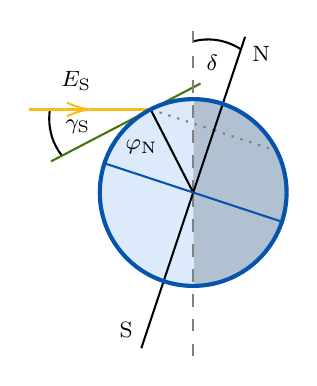
\begin{tikzpicture}[x=0.75pt,y=0.75pt,yscale=-1,xscale=1]
%uncomment if require: \path (0,201); %set diagram left start at 0, and has height of 201

%Shape: Pie [id:dp4750642586964353] 
\draw  [color={rgb, 255:red, 0; green, 0; blue, 0 }  ,draw opacity=0 ][fill={rgb, 255:red, 0; green, 0; blue, 0 }  ,fill opacity=0.45 ] (93.03,60.03) .. controls (117.81,60.3) and (137.85,80.25) .. (137.93,104.89) .. controls (138.02,129.63) and (117.94,149.78) .. (93.03,150.05) -- (92.52,105.04) -- cycle ;
%Shape: Circle [id:dp9006978183202985] 
\draw  [color={rgb, 255:red, 7; green, 84; blue, 173 }  ,draw opacity=1 ][fill={rgb, 255:red, 200; green, 222; blue, 248 }  ,fill opacity=0.64 ][line width=0.75]  (47.52,105.04) .. controls (47.52,80.19) and (67.67,60.04) .. (92.52,60.04) .. controls (117.38,60.04) and (137.52,80.19) .. (137.52,105.04) .. controls (137.52,129.89) and (117.38,150.04) .. (92.52,150.04) .. controls (67.67,150.04) and (47.52,129.89) .. (47.52,105.04) -- cycle ;
%Straight Lines [id:da06282467353758259] 
\draw [color={rgb, 255:red, 65; green, 117; blue, 5 }  ,draw opacity=1 ]   (96.02,52.54) -- (72.02,65.04) ;
%Shape: Arc [id:dp49173933797962777] 
\draw  [draw opacity=0] (29.42,87.46) .. controls (28.29,86.06) and (27.29,84.54) .. (26.43,82.91) .. controls (23.51,77.38) and (22.61,71.21) .. (23.45,65.01) -- (66.02,62.04) -- cycle ; \draw   (29.42,87.46) .. controls (28.29,86.06) and (27.29,84.54) .. (26.43,82.91) .. controls (23.51,77.38) and (22.61,71.21) .. (23.45,65.01) ;
%Straight Lines [id:da6550544250175496] 
\draw [color={rgb, 255:red, 65; green, 117; blue, 5 }  ,draw opacity=1 ]   (24.02,90.04) -- (72.02,65.04) ;
%Shape: Arc [id:dp963370582460114] 
\draw  [draw opacity=0] (92.23,32.3) .. controls (94.76,31.6) and (97.38,31.25) .. (100.07,31.29) .. controls (105.67,31.35) and (110.94,33.08) .. (115.6,36.08) -- (99.52,76.04) -- cycle ; \draw   (92.23,32.3) .. controls (94.76,31.6) and (97.38,31.25) .. (100.07,31.29) .. controls (105.67,31.35) and (110.94,33.08) .. (115.6,36.08) ;
%Straight Lines [id:da058893605247020586] 
\draw [color={rgb, 255:red, 128; green, 128; blue, 128 }  ,draw opacity=1 ] [dash pattern={on 4.5pt off 4.5pt}]  (92.52,183.96) -- (92.52,105.04) ;
%Straight Lines [id:da5478983474017609] 
\draw [color={rgb, 255:red, 128; green, 128; blue, 128 }  ,draw opacity=1 ] [dash pattern={on 4.5pt off 4.5pt}]  (92.52,105.04) -- (92.52,26.12) ;
%Straight Lines [id:da4780085054484584] 
\draw [line width=0.75]    (72.02,65.04) -- (92.52,105.04) ;
%Straight Lines [id:da5291514924825897] 
\draw [color={rgb, 255:red, 128; green, 128; blue, 128 }  ,draw opacity=1 ] [dash pattern={on 0.84pt off 2.51pt}]  (102.52,75.04) -- (133.02,85.04) ;
%Straight Lines [id:da4294056374442512] 
\draw [color={rgb, 255:red, 128; green, 128; blue, 128 }  ,draw opacity=1 ] [dash pattern={on 0.84pt off 2.51pt}]  (72.02,65.04) -- (102.52,75.04) ;
%Straight Lines [id:da35119327320040794] 
\draw    (92.52,105.04) -- (67.52,180.04) ;
%Straight Lines [id:da9687000233514724] 
\draw    (117.52,30.04) -- (92.52,105.04) ;
%Straight Lines [id:da8818616046820387] 
\draw [color={rgb, 255:red, 7; green, 84; blue, 173 }  ,draw opacity=1 ]   (50.02,91.04) -- (92.52,105.04) ;
%Straight Lines [id:da4795343191360564] 
\draw [color={rgb, 255:red, 7; green, 84; blue, 173 }  ,draw opacity=1 ]   (92.52,105.04) -- (135.02,119.04) ;
%Straight Lines [id:da6396043564859444] 
\draw [color={rgb, 255:red, 248; green, 189; blue, 28 }  ,draw opacity=1 ]   (42.65,65.04) -- (72.02,65.04) ;
%Straight Lines [id:da3150442288480175] 
\draw [color={rgb, 255:red, 248; green, 189; blue, 28 }  ,draw opacity=1 ]   (13.27,65.04) -- (40.65,65.04) ;
\draw [shift={(42.65,65.04)}, rotate = 180] [color={rgb, 255:red, 248; green, 189; blue, 28 }  ,draw opacity=1 ][line width=0.75]    (10.93,-3.29) .. controls (6.95,-1.4) and (3.31,-0.3) .. (0,0) .. controls (3.31,0.3) and (6.95,1.4) .. (10.93,3.29)   ;
%Shape: Circle [id:dp4877206756511603] 
\draw  [color={rgb, 255:red, 7; green, 84; blue, 173 }  ,draw opacity=1 ][fill={rgb, 255:red, 200; green, 222; blue, 248 }  ,fill opacity=0 ][line width=1.5]  (47.52,105.04) .. controls (47.52,80.19) and (67.67,60.04) .. (92.52,60.04) .. controls (117.38,60.04) and (137.52,80.19) .. (137.52,105.04) .. controls (137.52,129.89) and (117.38,150.04) .. (92.52,150.04) .. controls (67.67,150.04) and (47.52,129.89) .. (47.52,105.04) -- cycle ;

% Text Node
\draw (58.52,78.4) node [anchor=north west][inner sep=0.75pt]  [font=\footnotesize]  {$\varphi _{\mathrm{N}}$};
% Text Node
\draw (97.52,37.44) node [anchor=north west][inner sep=0.75pt]  [font=\footnotesize]  {$\delta $};
% Text Node
\draw (29.52,68.44) node [anchor=north west][inner sep=0.75pt]  [font=\footnotesize]  {$\gamma _{\mathrm{S}}$};
% Text Node
\draw (27.52,45.4) node [anchor=north west][inner sep=0.75pt]  [font=\footnotesize]  {$E_{\mathrm{S}}$};
% Text Node
\draw (119.52,33.04) node [anchor=north west][inner sep=0.75pt]  [font=\footnotesize] [align=left] {N};
% Text Node
\draw (55.52,166.04) node [anchor=north west][inner sep=0.75pt]  [font=\footnotesize] [align=left] {S};


\end{tikzpicture}

			\caption{Northern latitude.}
		\end{subfigure}
		\begin{subfigure}[b]{0.3\linewidth}
			

\tikzset{every picture/.style={line width=0.75pt}} %set default line width to 0.75pt        

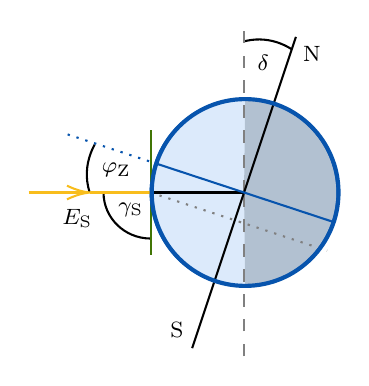
\begin{tikzpicture}[x=0.75pt,y=0.75pt,yscale=-1,xscale=1]
%uncomment if require: \path (0,181); %set diagram left start at 0, and has height of 181

%Shape: Arc [id:dp20953347708018688] 
\draw  [draw opacity=0] (69.43,111.09) .. controls (69.33,111.09) and (69.24,111.09) .. (69.15,111.09) .. controls (56.73,110.92) and (46.77,101.07) .. (46.73,89) -- (69.44,88.92) -- cycle ; \draw   (69.43,111.09) .. controls (69.33,111.09) and (69.24,111.09) .. (69.15,111.09) .. controls (56.73,110.92) and (46.77,101.07) .. (46.73,89) ;
%Shape: Arc [id:dp16591242877449974] 
\draw  [draw opacity=0] (40.06,88.92) .. controls (39.51,87.21) and (39.11,85.44) .. (38.89,83.61) .. controls (38.13,77.4) and (39.47,71.31) .. (42.46,65.81) -- (83.31,78.18) -- cycle ; \draw   (40.06,88.92) .. controls (39.51,87.21) and (39.11,85.44) .. (38.89,83.61) .. controls (38.13,77.4) and (39.47,71.31) .. (42.46,65.81) ;
%Straight Lines [id:da6013522376382066] 
\draw [color={rgb, 255:red, 65; green, 117; blue, 5 }  ,draw opacity=1 ]   (69.44,118.92) -- (69.44,88.92) ;
%Shape: Pie [id:dp028486029029515914] 
\draw  [color={rgb, 255:red, 0; green, 0; blue, 0 }  ,draw opacity=0 ][fill={rgb, 255:red, 0; green, 0; blue, 0 }  ,fill opacity=0.45 ] (114.95,43.91) .. controls (139.73,44.18) and (159.77,64.13) .. (159.85,88.77) .. controls (159.93,113.51) and (139.86,133.66) .. (114.94,133.93) -- (114.44,88.92) -- cycle ;
%Shape: Circle [id:dp7286185522053927] 
\draw  [color={rgb, 255:red, 7; green, 84; blue, 173 }  ,draw opacity=1 ][fill={rgb, 255:red, 200; green, 222; blue, 248 }  ,fill opacity=0.64 ][line width=0.75]  (69.44,88.92) .. controls (69.44,64.07) and (89.59,43.92) .. (114.44,43.92) .. controls (139.29,43.92) and (159.44,64.07) .. (159.44,88.92) .. controls (159.44,113.77) and (139.29,133.92) .. (114.44,133.92) .. controls (89.59,133.92) and (69.44,113.77) .. (69.44,88.92) -- cycle ;
%Shape: Arc [id:dp17913789171454497] 
\draw  [draw opacity=0] (114.15,16.18) .. controls (116.67,15.49) and (119.3,15.14) .. (121.99,15.17) .. controls (127.58,15.24) and (132.85,16.96) .. (137.52,19.97) -- (121.44,59.92) -- cycle ; \draw   (114.15,16.18) .. controls (116.67,15.49) and (119.3,15.14) .. (121.99,15.17) .. controls (127.58,15.24) and (132.85,16.96) .. (137.52,19.97) ;
%Straight Lines [id:da9967059081670446] 
\draw [color={rgb, 255:red, 128; green, 128; blue, 128 }  ,draw opacity=1 ] [dash pattern={on 4.5pt off 4.5pt}]  (114.44,167.84) -- (114.44,88.92) ;
%Straight Lines [id:da71597890822506] 
\draw [color={rgb, 255:red, 128; green, 128; blue, 128 }  ,draw opacity=1 ] [dash pattern={on 4.5pt off 4.5pt}]  (114.44,88.92) -- (114.44,10) ;
%Straight Lines [id:da4137878061890663] 
\draw [color={rgb, 255:red, 128; green, 128; blue, 128 }  ,draw opacity=1 ] [dash pattern={on 0.84pt off 2.51pt}]  (69.44,88.92) -- (111.94,102.92) ;
%Straight Lines [id:da3390187694217488] 
\draw [color={rgb, 255:red, 128; green, 128; blue, 128 }  ,draw opacity=1 ] [dash pattern={on 0.84pt off 2.51pt}]  (111.94,102.92) -- (154.44,116.92) ;
%Straight Lines [id:da5052190602488993] 
\draw    (114.44,88.92) -- (89.44,163.92) ;
%Straight Lines [id:da6983846735857875] 
\draw    (139.44,13.92) -- (114.44,88.92) ;
%Straight Lines [id:da5175201690882127] 
\draw    (69.44,88.92) -- (114.44,88.92) ;
%Straight Lines [id:da23163800871480023] 
\draw [color={rgb, 255:red, 65; green, 117; blue, 5 }  ,draw opacity=1 ]   (69.44,88.92) -- (69.44,58.92) ;
%Straight Lines [id:da47404926603772557] 
\draw [color={rgb, 255:red, 7; green, 84; blue, 173 }  ,draw opacity=1 ] [dash pattern={on 0.84pt off 2.51pt}]  (29.44,60.92) -- (71.94,74.92) ;
%Straight Lines [id:da6548182479176137] 
\draw [color={rgb, 255:red, 248; green, 189; blue, 28 }  ,draw opacity=1 ]   (10.69,88.92) -- (38.06,88.92) ;
\draw [shift={(40.06,88.92)}, rotate = 180] [color={rgb, 255:red, 248; green, 189; blue, 28 }  ,draw opacity=1 ][line width=0.75]    (10.93,-3.29) .. controls (6.95,-1.4) and (3.31,-0.3) .. (0,0) .. controls (3.31,0.3) and (6.95,1.4) .. (10.93,3.29)   ;
%Straight Lines [id:da7518207882403078] 
\draw [color={rgb, 255:red, 248; green, 189; blue, 28 }  ,draw opacity=1 ]   (40.06,88.92) -- (69.44,88.92) ;
%Shape: Circle [id:dp4417291051670942] 
\draw  [color={rgb, 255:red, 7; green, 84; blue, 173 }  ,draw opacity=1 ][fill={rgb, 255:red, 200; green, 222; blue, 248 }  ,fill opacity=0 ][line width=1.5]  (69.95,88.91) .. controls (69.95,64.06) and (90.1,43.91) .. (114.95,43.91) .. controls (139.8,43.91) and (159.95,64.06) .. (159.95,88.91) .. controls (159.95,113.77) and (139.8,133.91) .. (114.95,133.91) .. controls (90.1,133.91) and (69.95,113.77) .. (69.95,88.91) -- cycle ;
%Straight Lines [id:da09584357360735729] 
\draw [color={rgb, 255:red, 7; green, 84; blue, 173 }  ,draw opacity=1 ]   (71.94,74.92) -- (114.44,88.92) ;
%Straight Lines [id:da1322107965109387] 
\draw [color={rgb, 255:red, 7; green, 84; blue, 173 }  ,draw opacity=1 ]   (114.44,88.92) -- (156.94,102.92) ;

% Text Node
\draw (44.44,73.32) node [anchor=north west][inner sep=0.75pt]  [font=\footnotesize]  {$\varphi _{\mathrm{Z}}$};
% Text Node
\draw (119.44,21.32) node [anchor=north west][inner sep=0.75pt]  [font=\footnotesize]  {$\delta $};
% Text Node
\draw (25.44,95.4) node [anchor=north west][inner sep=0.75pt]  [font=\footnotesize]  {$E_{\mathrm{S}}$};
% Text Node
\draw (141.44,16.92) node [anchor=north west][inner sep=0.75pt]  [font=\footnotesize] [align=left] {N};
% Text Node
\draw (77.44,149.92) node [anchor=north west][inner sep=0.75pt]  [font=\footnotesize] [align=left] {S};
% Text Node
\draw (52.44,92.32) node [anchor=north west][inner sep=0.75pt]  [font=\footnotesize]  {$\gamma _{\mathrm{S}}$};


\end{tikzpicture}

			\caption{Sun is at its zenith.}
		\end{subfigure}
		\begin{subfigure}[b]{0.3\linewidth}
			

\tikzset{every picture/.style={line width=0.75pt}} %set default line width to 0.75pt        

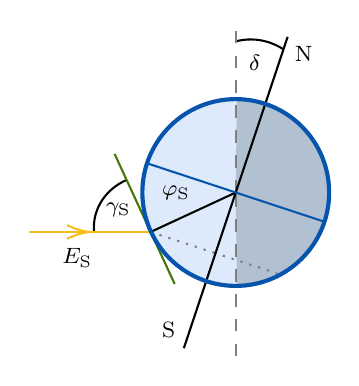
\begin{tikzpicture}[x=0.75pt,y=0.75pt,yscale=-1,xscale=1]
%uncomment if require: \path (0,181); %set diagram left start at 0, and has height of 181

%Shape: Arc [id:dp1509931683753729] 
\draw  [draw opacity=0] (41.51,107.98) .. controls (41.44,107.22) and (41.4,106.45) .. (41.4,105.68) .. controls (41.4,95.62) and (47.84,86.94) .. (57.17,82.86) -- (69.17,105.68) -- cycle ; \draw   (41.51,107.98) .. controls (41.44,107.22) and (41.4,106.45) .. (41.4,105.68) .. controls (41.4,95.62) and (47.84,86.94) .. (57.17,82.86) ;
%Shape: Pie [id:dp008234319355738817] 
\draw  [color={rgb, 255:red, 0; green, 0; blue, 0 }  ,draw opacity=0 ][fill={rgb, 255:red, 0; green, 0; blue, 0 }  ,fill opacity=0.45 ] (110.26,43.91) .. controls (135.04,44.18) and (155.08,64.13) .. (155.16,88.77) .. controls (155.24,113.51) and (135.17,133.66) .. (110.25,133.93) -- (109.75,88.92) -- cycle ;
%Shape: Circle [id:dp3321431212746069] 
\draw  [color={rgb, 255:red, 7; green, 84; blue, 173 }  ,draw opacity=1 ][fill={rgb, 255:red, 200; green, 222; blue, 248 }  ,fill opacity=0.64 ][line width=0.75]  (64.75,88.92) .. controls (64.75,64.07) and (84.9,43.92) .. (109.75,43.92) .. controls (134.6,43.92) and (154.75,64.07) .. (154.75,88.92) .. controls (154.75,113.77) and (134.6,133.92) .. (109.75,133.92) .. controls (84.9,133.92) and (64.75,113.77) .. (64.75,88.92) -- cycle ;
%Straight Lines [id:da8319048303736489] 
\draw [color={rgb, 255:red, 65; green, 117; blue, 5 }  ,draw opacity=1 ]   (57.17,82.86) -- (68.75,107.92) ;
%Shape: Arc [id:dp7416942399851174] 
\draw  [draw opacity=0] (109.46,16.18) .. controls (111.99,15.49) and (114.61,15.14) .. (117.3,15.17) .. controls (122.89,15.24) and (128.16,16.96) .. (132.83,19.97) -- (116.75,59.92) -- cycle ; \draw   (109.46,16.18) .. controls (111.99,15.49) and (114.61,15.14) .. (117.3,15.17) .. controls (122.89,15.24) and (128.16,16.96) .. (132.83,19.97) ;
%Straight Lines [id:da23785833539369183] 
\draw [color={rgb, 255:red, 128; green, 128; blue, 128 }  ,draw opacity=1 ] [dash pattern={on 4.5pt off 4.5pt}]  (109.75,167.84) -- (109.75,88.92) ;
%Straight Lines [id:da06972248148475568] 
\draw [color={rgb, 255:red, 128; green, 128; blue, 128 }  ,draw opacity=1 ] [dash pattern={on 4.5pt off 4.5pt}]  (109.75,88.92) -- (109.75,10) ;
%Straight Lines [id:da8960602024330377] 
\draw [line width=0.75]    (68.75,107.92) -- (109.75,88.92) ;
%Straight Lines [id:da5098060920131091] 
\draw [color={rgb, 255:red, 128; green, 128; blue, 128 }  ,draw opacity=1 ] [dash pattern={on 0.84pt off 2.51pt}]  (99.25,117.92) -- (129.75,127.92) ;
%Straight Lines [id:da8906380552334501] 
\draw [color={rgb, 255:red, 128; green, 128; blue, 128 }  ,draw opacity=1 ] [dash pattern={on 0.84pt off 2.51pt}]  (68.75,107.92) -- (99.25,117.92) ;
%Straight Lines [id:da14349690184184327] 
\draw    (109.75,88.92) -- (84.75,163.92) ;
%Straight Lines [id:da024036142327008347] 
\draw    (134.75,13.92) -- (109.75,88.92) ;
%Straight Lines [id:da21245027564913532] 
\draw [color={rgb, 255:red, 7; green, 84; blue, 173 }  ,draw opacity=1 ]   (67.25,74.92) -- (109.75,88.92) ;
%Straight Lines [id:da7748765899346521] 
\draw [color={rgb, 255:red, 7; green, 84; blue, 173 }  ,draw opacity=1 ]   (109.75,88.92) -- (152.25,102.92) ;
%Straight Lines [id:da645165483038932] 
\draw [color={rgb, 255:red, 65; green, 117; blue, 5 }  ,draw opacity=1 ]   (68.75,107.92) -- (80.33,132.98) ;
%Straight Lines [id:da01702325380082992] 
\draw [color={rgb, 255:red, 65; green, 117; blue, 5 }  ,draw opacity=1 ]   (57.17,82.86) -- (51.38,70.33) ;
%Straight Lines [id:da7674893611261671] 
\draw [color={rgb, 255:red, 248; green, 189; blue, 28 }  ,draw opacity=1 ]   (39.38,107.92) -- (68.75,107.92) ;
%Straight Lines [id:da5473156330354862] 
\draw [color={rgb, 255:red, 248; green, 189; blue, 28 }  ,draw opacity=1 ]   (10,107.92) -- (37.38,107.92) ;
\draw [shift={(39.38,107.92)}, rotate = 180] [color={rgb, 255:red, 248; green, 189; blue, 28 }  ,draw opacity=1 ][line width=0.75]    (10.93,-3.29) .. controls (6.95,-1.4) and (3.31,-0.3) .. (0,0) .. controls (3.31,0.3) and (6.95,1.4) .. (10.93,3.29)   ;
%Shape: Circle [id:dp46167221588038543] 
\draw  [color={rgb, 255:red, 7; green, 84; blue, 173 }  ,draw opacity=1 ][fill={rgb, 255:red, 200; green, 222; blue, 248 }  ,fill opacity=0 ][line width=1.5]  (64.75,88.92) .. controls (64.75,64.07) and (84.9,43.92) .. (109.75,43.92) .. controls (134.6,43.92) and (154.75,64.07) .. (154.75,88.92) .. controls (154.75,113.77) and (134.6,133.92) .. (109.75,133.92) .. controls (84.9,133.92) and (64.75,113.77) .. (64.75,88.92) -- cycle ;

% Text Node
\draw (72.75,84.32) node [anchor=north west][inner sep=0.75pt]  [font=\footnotesize]  {$\varphi _{\mathrm{S}}$};
% Text Node
\draw (114.75,21.32) node [anchor=north west][inner sep=0.75pt]  [font=\footnotesize]  {$\delta $};
% Text Node
\draw (45.75,92.32) node [anchor=north west][inner sep=0.75pt]  [font=\footnotesize]  {$\gamma _{\mathrm{S}}$};
% Text Node
\draw (24.75,114.32) node [anchor=north west][inner sep=0.75pt]  [font=\footnotesize]  {$E_{\mathrm{S}}$};
% Text Node
\draw (136.75,16.92) node [anchor=north west][inner sep=0.75pt]  [font=\footnotesize] [align=left] {N};
% Text Node
\draw (72.75,149.92) node [anchor=north west][inner sep=0.75pt]  [font=\footnotesize] [align=left] {S};


\end{tikzpicture}

			\caption{Southern latitude.}
		\end{subfigure}
	\caption{Illustration of the latitude $\varphi_{\mathrm{Z}}$ on Earth at which the Sun is at its zenith for $t_{\mathrm{S}} = 12\mathrm{h}$. By comparing the latitude of the installation site of a photovoltaic generator it can be determined how it must be aligned, so that the electrical energy yield can be maximized.}
	\label{fig:crucial_latitudes}
\end{figure}

Inserting $\gamma_{\mathrm{S}} = 90^\circ$ and $t_{\mathrm{S}} = 12\mathrm{h}$ into equation (\ref{eq:sin_gamma_s}), the latitude $\varphi_{\mathrm{Z}}$ can be determined -- after applying trigonometric functions -- to:
	\begin{equation} \label{eq:phi_z}
	\centering
		\varphi_{\mathrm{Z}} = \delta \text{.}
	\end{equation}
If a PV generator is installed at a latitude south of $\varphi_{\mathrm{Z}}$, the normal to $A_{\mathrm{PV}}$ must point towards the north, and if it is installed north of $\varphi_{\mathrm{Z}}$, the normal to $A_{\mathrm{PV}}$ must point towards the south. In case the PV generator is installed at the latitude $\varphi_{\mathrm{Z}}$, then $\beta = \varphi_{\mathrm{Z}} - \delta = 0^\circ$ applies, which means that the normal to $A_{\mathrm{PV}}$ points to the Sun's zenith. The normal to $A_{\mathrm{PV}}$ can be aligned using a simple compass.

\subsection{Modeling the solar energy curve} \label{sec:solar_energy_curve}
To further estimate the electrical energy yield of a PV generator which is inclined with the angle $\beta$, the Sun's radiation flux $\Phi_{\mathrm{G}}$ onto its energy-converting area $A_{\mathrm{PV}}$ must be modeled over the course of one day. Since the Sun's irradiance is symmetrical for $t_0 = 12\mathrm{h}$ and the PV generator is assumed to be aligned so that $A_{\mathrm{PV}}$ is perpendicular to the Sun's rays for $t_0 = 12\mathrm{h}$, the Sun's radiation flux $\Phi_{\mathrm{G}}$ as a Gaussian function of the solar time $t_{\mathrm{S}}$ can be approximated as shown in the figure \ref{fig:tikz_energy_gauss}.
\begin{figure}[h!]
	\centering
	

\tikzset{every picture/.style={line width=0.75pt}} %set default line width to 0.75pt        

\begin{tikzpicture}[x=0.75pt,y=0.75pt,yscale=-1,xscale=1]
%uncomment if require: \path (0,300); %set diagram left start at 0, and has height of 300

%Image [id:dp32150908690987645] 
\draw (327,150) node  {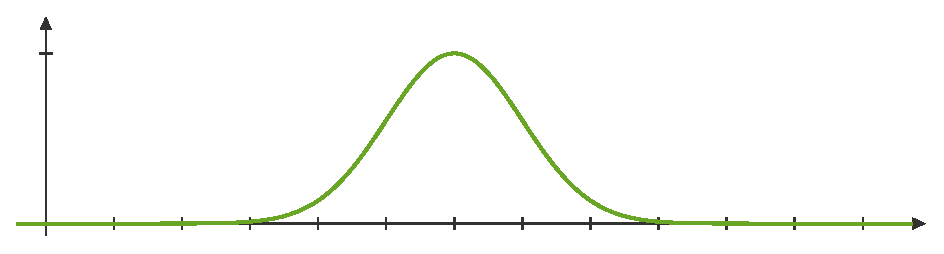
\includegraphics[width=439.5pt,height=105pt]{images/image_energy_gauss}};
%Straight Lines [id:da07666169968429992] 
\draw [color={rgb, 255:red, 155; green, 155; blue, 155 }  ,draw opacity=1 ] [dash pattern={on 4.5pt off 4.5pt}]  (63,103.4) -- (306,103.4) ;
%Straight Lines [id:da12384412498194441] 
\draw [color={rgb, 255:red, 155; green, 155; blue, 155 }  ,draw opacity=1 ] [dash pattern={on 4.5pt off 4.5pt}]  (315.6,201) -- (315.6,103) ;
%Shape: Circle [id:dp581375357919033] 
\draw  [fill={rgb, 255:red, 255; green, 255; blue, 255 }  ,fill opacity=1 ] (313.6,103.5) .. controls (313.6,102.4) and (314.5,101.5) .. (315.6,101.5) .. controls (316.7,101.5) and (317.6,102.4) .. (317.6,103.5) .. controls (317.6,104.6) and (316.7,105.5) .. (315.6,105.5) .. controls (314.5,105.5) and (313.6,104.6) .. (313.6,103.5) -- cycle ;

% Text Node
\draw (626,205.4) node [anchor=north west][inner sep=0.75pt]  [font=\footnotesize]  {$t_{\mathrm{S}}$};
% Text Node
\draw (34,59.4) node [anchor=north west][inner sep=0.75pt]  [font=\footnotesize]  {$\Phi _{\mathrm{G}}( t_{\mathrm{S}})$};
% Text Node
\draw (15,97.4) node [anchor=north west][inner sep=0.75pt]  [font=\footnotesize]  {$\Phi _{\mathrm{max}}$};
% Text Node
\draw (143,220.4) node [anchor=north west][inner sep=0.75pt]  [font=\footnotesize]  {$t_{\mathrm{S,r}} =t_{0} -3\tau _{\mathrm{S}}$};
% Text Node
\draw (162,240) node [anchor=north west][inner sep=0.75pt]  [font=\footnotesize] [align=left] {Sunrise};
% Text Node
\draw (298,240) node [anchor=north west][inner sep=0.75pt]  [font=\footnotesize] [align=left] {Noon};
% Text Node
\draw (287.5,220.4) node [anchor=north west][inner sep=0.75pt]  [font=\footnotesize]  {$t_{0} =12\mathrm{h}$};
% Text Node
\draw (403.1,220.4) node [anchor=north west][inner sep=0.75pt]  [font=\footnotesize]  {$t_{\mathrm{S,s}} =t_{0} +3\tau _{\mathrm{S}}$};
% Text Node
\draw (424,240) node [anchor=north west][inner sep=0.75pt]  [font=\footnotesize] [align=left] {Sunset};
% Text Node
\draw (564,220.4) node [anchor=north west][inner sep=0.75pt]  [font=\footnotesize]  {$2t_{0}$};
% Text Node
\draw (551,240) node [anchor=north west][inner sep=0.75pt]  [font=\footnotesize] [align=left] {Midnight};
% Text Node
\draw (44,220.4) node [anchor=north west][inner sep=0.75pt]  [font=\footnotesize]  {$0\mathrm{h}$};
% Text Node
\draw (14,240) node [anchor=north west][inner sep=0.75pt]  [font=\footnotesize] [align=left] {New solar day};


\end{tikzpicture}



	\caption{Model of the Sun's radiation flux $\Phi_{\mathrm{G}}$ onto the energy-converting area of a photovoltaic generator as a Gaussain function of the solar time $t_{\mathrm{S}}$. It is assumed that the Sun's irradiance is symmetrical around solar noon, and that the photovoltaic generator is aligned so that its energy-converting area is perpendicular to the Sun's rays at solar noon.}
	\label{fig:tikz_energy_gauss}
\end{figure}
The corresponding Gaussian function can be obtained from equation (\ref{eq:phi_gen_gauss}):
	\begin{equation} \label{eq:phi_gen_gauss}
	\centering
		\begin{gathered}
		\Phi_{\mathrm{G}}\left(t_{\mathrm{S}}\right) = \Phi_{\mathrm{max}} \, \exp\left(-\frac{(t_{\mathrm{S}} - t_0)^2}{2 \tau_\mathrm{S}^2}\right) \text{, } 
		\\
		\tau_\mathrm{S} = \frac{t_0 - t_{\mathrm{S,r}}}{3} = \frac{t_{\mathrm{S,s}} - t_0}{3} \text{.}
		\end{gathered}
	\end{equation}
The area this curve encloses with the solar time axis $t_{\mathrm{S}}$, from solar sunrise $t_{\mathrm{S,r}}$ to solar sunset $t_{\mathrm{S,s}}$, is equal to 99,7\% of the \emph{daily solar energy} $W_{\mathrm{G}}$ in $\left(\mathrm{Wh}\right)$ which occurs on the energy-converting area $A_{\mathrm{PV}}$ \cite{Landis:1995, Prechtl:2006, Prechtl:2008, Glover:2010, Schrufer:2014, AlNahhal:2019}:\footnote{$t_{\mathrm{S,r}}$ and $t_{\mathrm{S,s}}$ were selected this way for simplicity.}
	\begin{equation} \label{eq:w_gen_gauss}
	\centering
		W_\mathrm{G} = \frac{1}{0,997} \int\limits_{t_{\mathrm{S,r}}}^{t_{\mathrm{S,s}}} \Phi_{\mathrm{max}} \, \exp\left(-\frac{(t_{\mathrm{S}} - t_0)^2}{2 \tau_\mathrm{S}^2}\right) \,\mathrm{d}t_\mathrm{S} = \frac{\Phi_{\mathrm{max}} \, \tau_\mathrm{S} \sqrt{2\pi}}{0,997} \text{.}
	\end{equation}

A similar approach is used in \cite{Guo:2017, Nguyen:2020} and in \cite{Balafas:2010, Mertens:2015, Koudouris:2017} it can be seen that the Sun's total irradiance $E_{\mathrm{G}}$ throughout the day, from which $\Phi_{\mathrm{G}}$ derives, behaves similar to a Gaussian curve.\footnote{How to solve the integral in equation \ref{eq:w_gen_gauss} from $-\infty$ to $\infty$ can be found in the appendix \ref{sec:gauss_general}.}

The greates daily radiation flux $\Phi_{\mathrm{max}}$ in $\left(\mathrm W\right)$ onto $A_{\mathrm{PV}}$ can be calculated using the equations (\ref{eq:e_gen_ghi_dni}) and (\ref{eq:radiation_flux}) by deriving the following relationship:
	\begin{equation} \label{eq:w_gen}
	\centering
		W_\mathrm{G} = \int\limits_{t_{\mathrm{S,r}}}^{t_{\mathrm{S,s}}} \Phi_{\mathrm{G}}\,\mathrm{d}t_\mathrm{S} = A_{\mathrm{PV}} \int\limits_{t_{\mathrm{S,r}}}^{t_{\mathrm{S,s}}} E_{\mathrm{G}}\,\mathrm{d}t_\mathrm{S} \text{.}
	\end{equation}
Considering that $A_{\mathrm{PV}}$ is a constant factor and taking into account the findings from the subsection \ref{sec:energy_yield}, the integrals from equation (\ref{eq:w_gen}) can be partly solved as follows:
	\begin{equation} \label{eq:int_e_gen}
	\centering
		\begin{split}
		\int\limits_{t_{\mathrm{S,r}}}^{t_{\mathrm{S,s}}} E_{\mathrm{G}}\,\mathrm{d}t_\mathrm{S} = E_{\mathrm{GHI}} \left( \frac{1 + \cos \beta}{2} + \frac{1 - \cos \beta}{2} \cdot \mathrm{ALB} \right) \cdot \left(t_{\mathrm{S,s}} - t_{\mathrm{S,r}}\right) \\ 
		- E_{\mathrm{DNI}} \ \frac{1 + \cos \beta}{2} \underbrace{\int\limits_{t_{\mathrm{S,r}}}^{t_{\mathrm{S,s}}} \sin \gamma_{\mathrm{S}}\,\mathrm{d}t_\mathrm{S}}_\text{\textbf{\RN{1}}} + E_{\mathrm{DNI}} \underbrace{\int\limits_{t_{\mathrm{S,r}}}^{t_{\mathrm{S,s}}} \cos \theta \,\mathrm{d}t_\mathrm{S}}_\text{\textbf{\RN{2}}} \text{.}
		\end{split}
	\end{equation}
Using the equations (\ref{eq:sin_gamma_s}) and (\ref{eq:solar_hour_angle}), integral \text{\textbf{\RN{1}}} can be solved to:
	\begin{equation} \label{eq:int_rn_1}
	\centering
		\begin{aligned}
		\text{\textbf{\RN{1}}:} \ &\int\limits_{t_{\mathrm{S,r}}}^{t_{\mathrm{S,s}}} \sin \gamma_{\mathrm{S}}\,\mathrm{d}t_\mathrm{S} = 
		\sin \varphi \, \sin \delta \left(t_{\mathrm{S,s}} - t_{\mathrm{S,r}} \right) \\
		&+ c_{\varphi,\delta} \left(\sin \left(\left(t_{\mathrm{S,s}} - 12\mathrm{h} \right) \cdot \frac{15^\circ}{1\mathrm{h}} \right) - \sin \left(\left( t_{\mathrm{S,r}} - 12\mathrm{h} \right) \cdot \frac{15^\circ}{1\mathrm{h}} \right)\right) \text{,}
		\end{aligned}
	\end{equation}
with $c_{\varphi,\delta}$ being:
	\begin{equation} \label{eq:const_varphi_delta}
	\centering
		c_{\varphi,\delta} = \cos \varphi \, \cos \delta \cdot \frac{1\mathrm{h}}{15^\circ} \text{.}
	\end{equation}
Integral \text{\textbf{\RN{2}}} on the other hand cannot be solved analytically as easy. This is why a sum instead of an integral is used in the \MATLAB simulation (see appendix \ref{sec:matlab_code}) to calculate $W_{\mathrm{G}}$:
	\begin{equation} \label{eq:sum_energy}
	\centering
		W_\mathrm{G} = A_{\mathrm{PV}} \displaystyle\sum_{t_{\mathrm{S}} = t_{\mathrm{S,r}}}^{t_{\mathrm{S,s}}} E_{\mathrm{G}} \, \Delta t_{\mathrm{S}} \text{.}
	\end{equation}
Using trigonometric functions, $E_{\mathrm{G}}$ can be simplyfied as shown in the equation (\ref{eq:sum_e_gen}). Depending on the desired accuracy $\Delta t_{\mathrm{S}}$ in $\left( \mathrm{h} \right)$ can be smaller or greater. The smaller it is the more accurate $W_{\mathrm{G}}$ can be modeled.\footnote{$\Delta t_{\mathrm{S}}$ is one discrete time step of the solar time. It can be caluculated from the length $len$ of the Matlab vector that goes from $t_{\mathrm{S,r}}$ to $t_{\mathrm{S,s}}$: $\Delta t_{\mathrm{S}} = \frac{1}{len}$.}
	\begin{equation} \label{eq:sum_e_gen}
	\centering
		\begin{aligned}
		\displaystyle\sum_{t_{\mathrm{S}} = t_{\mathrm{S,r}}}^{t_{\mathrm{S,s}}} E_{\mathrm{G}} \, \Delta t_{\mathrm{S}} &= \displaystyle\sum_{t_{\mathrm{S}} = t_{\mathrm{S,r}}}^{t_{\mathrm{S,s}}} \left(E_{\mathrm{GHI}} - E_{\mathrm{DNI}} \, \sin \gamma_{\mathrm{S}} \right) \cos^2 \frac{\beta}{2} \, \Delta t_{\mathrm{S}} \\
		&+ \displaystyle\sum_{t_{\mathrm{S}} = t_{\mathrm{S,r}}}^{t_{\mathrm{S,s}}} \left(E_{\mathrm{DNI}} \, \cos \theta + E_{\mathrm{GHI}} \, \sin^2 \frac{\beta}{2} \cdot \mathrm{ALB} \right)\Delta t_{\mathrm{S}}
		\end{aligned}
	\end{equation}
By inserting the caluclated $W_{\mathrm{G}}$ from equation (\ref{eq:sum_energy}) into equation (\ref{eq:w_gen_gauss}) and transforming it, the greates daily radiation flux $\Phi_{\mathrm{max}}$ onto $A_{\mathrm{PV}}$, which in this model occurs for $t_0 = 12\mathrm{h}$, can be obtained \cite{Appelbaum:1992, Landis:1995, Prechtl:2006, Prechtl:2008}:
	\begin{equation} \label{eq:phi_max_sum}
	\centering
		\Phi_{\mathrm{max}} = \frac{0,997 \cdot A_{\mathrm{PV}}}{\tau_\mathrm{S} \sqrt{2\pi}} \displaystyle\sum_{t_{\mathrm{S}} = t_{\mathrm{S,r}}}^{t_{\mathrm{S,s}}} E_{\mathrm{G}} \, \Delta t_{\mathrm{S}} \text{.}
	\end{equation}

\subsection{Photovoltaic generators} \label{sec:photovoltaic_generators}
The aim of this subsection is to model the \emph{electrical power output} $P_{\mathrm{PV}}$ in $\left( \mathrm W \right)$ of a PV generator based on the previous findings. Since most commercial PV generators consist of PV cells connected in series, only these are going to be covered. Figure \ref{fig:tikz_PVG_circuit_diagram} shows the \emph{electrical equivalent circuit} (EEC) of such a PV generator with a given \emph{number of PV cells} $N_{\mathrm{C}}$ in $\left( 1 \right)$.
\begin{figure}[h!]
	\centering
	

\tikzset{every picture/.style={line width=0.75pt}} %set default line width to 0.75pt        

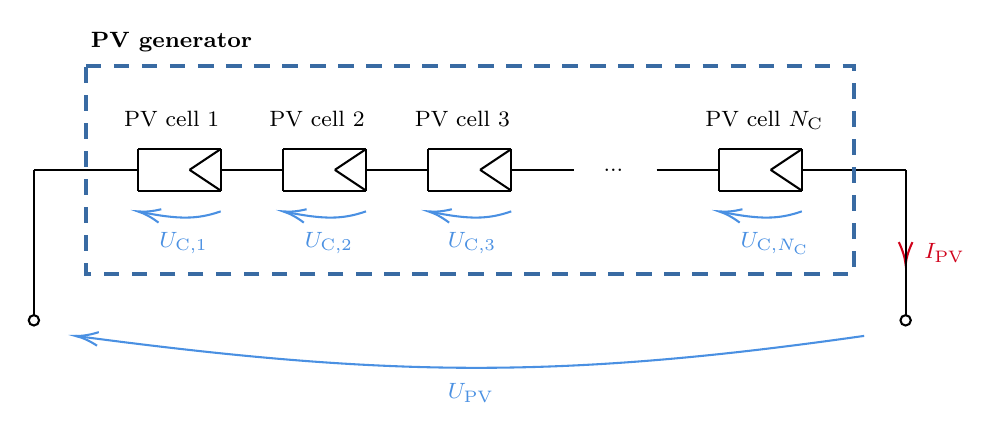
\begin{tikzpicture}[x=0.75pt,y=0.75pt,yscale=-1,xscale=1]
%uncomment if require: \path (0,300); %set diagram left start at 0, and has height of 300

%Straight Lines [id:da607551945482224] 
\draw [color={rgb, 255:red, 208; green, 2; blue, 27 }  ,draw opacity=1 ]   (560,180) -- (560,193.75) ;
\draw [shift={(560,195.75)}, rotate = 270] [color={rgb, 255:red, 208; green, 2; blue, 27 }  ,draw opacity=1 ][line width=0.75]    (10.93,-3.29) .. controls (6.95,-1.4) and (3.31,-0.3) .. (0,0) .. controls (3.31,0.3) and (6.95,1.4) .. (10.93,3.29)   ;
%Straight Lines [id:da39220891738716435] 
\draw    (370,140) -- (370,160) ;
%Straight Lines [id:da26376681003549773] 
\draw    (370,140) -- (355,150) ;
%Straight Lines [id:da7171194033958681] 
\draw    (355,150) -- (370,160) ;
%Straight Lines [id:da7758232590553849] 
\draw    (370,140) -- (330,140) ;
%Straight Lines [id:da23922780724985704] 
\draw    (370,160) -- (330,160) ;
%Straight Lines [id:da8647396746050291] 
\draw    (330,140) -- (330,160) ;
%Shape: Circle [id:dp9465717065223571] 
\draw   (560,220) .. controls (561.38,220) and (562.5,221.12) .. (562.5,222.5) .. controls (562.5,223.88) and (561.38,225) .. (560,225) .. controls (558.62,225) and (557.5,223.88) .. (557.5,222.5) .. controls (557.5,221.12) and (558.62,220) .. (560,220) -- cycle ;
%Straight Lines [id:da8361729954042678] 
\draw    (300,140) -- (300,160) ;
%Straight Lines [id:da8303503310697085] 
\draw    (300,140) -- (285,150) ;
%Straight Lines [id:da6935206293495084] 
\draw    (285,150) -- (300,160) ;
%Straight Lines [id:da4478328338561339] 
\draw    (300,140) -- (260,140) ;
%Straight Lines [id:da6338115192168345] 
\draw    (300,160) -- (260,160) ;
%Straight Lines [id:da4710313866121387] 
\draw    (260,140) -- (260,160) ;
%Straight Lines [id:da04529427678773623] 
\draw    (510,140) -- (510,160) ;
%Straight Lines [id:da12585917694032633] 
\draw    (510,140) -- (495,150) ;
%Straight Lines [id:da5777912998057524] 
\draw    (495,150) -- (510,160) ;
%Straight Lines [id:da8526647582658238] 
\draw    (510,140) -- (470,140) ;
%Straight Lines [id:da18181567227521733] 
\draw    (510,160) -- (470,160) ;
%Straight Lines [id:da08821152259447507] 
\draw    (470,140) -- (470,160) ;
%Straight Lines [id:da004318261204414364] 
\draw    (300,150) -- (330,150) ;
%Straight Lines [id:da415576466861697] 
\draw    (440,150) -- (470,150) ;
%Straight Lines [id:da5030082829613725] 
\draw    (230,140) -- (230,160) ;
%Straight Lines [id:da24153450583970604] 
\draw    (230,140) -- (215,150) ;
%Straight Lines [id:da7169826080141817] 
\draw    (215,150) -- (230,160) ;
%Straight Lines [id:da8893075482646204] 
\draw    (230,140) -- (190,140) ;
%Straight Lines [id:da8414185658377555] 
\draw    (230,160) -- (190,160) ;
%Straight Lines [id:da030501270201809483] 
\draw    (190,140) -- (190,160) ;
%Straight Lines [id:da11000547395248828] 
\draw    (140,150) -- (190,150) ;
%Straight Lines [id:da8573962154803463] 
\draw    (230,150) -- (260,150) ;
%Straight Lines [id:da9793828451968309] 
\draw    (370,150) -- (400,150) ;
%Straight Lines [id:da6281863128480734] 
\draw    (510,150) -- (560,150) ;
%Shape: Rectangle [id:dp583588773515656] 
\draw  [color={rgb, 255:red, 57; green, 107; blue, 163 }  ,draw opacity=1 ][dash pattern={on 5.63pt off 4.5pt}][line width=1.5]  (165,100) -- (535,100) -- (535,200) -- (165,200) -- cycle ;
%Curve Lines [id:da418839437477464] 
\draw [color={rgb, 255:red, 74; green, 144; blue, 226 }  ,draw opacity=1 ]   (230,170) .. controls (218.85,173.88) and (210.04,174) .. (191.73,170.35) ;
\draw [shift={(190,170)}, rotate = 371.59000000000003] [color={rgb, 255:red, 74; green, 144; blue, 226 }  ,draw opacity=1 ][line width=0.75]    (10.93,-3.29) .. controls (6.95,-1.4) and (3.31,-0.3) .. (0,0) .. controls (3.31,0.3) and (6.95,1.4) .. (10.93,3.29)   ;
%Curve Lines [id:da498717897550782] 
\draw [color={rgb, 255:red, 74; green, 144; blue, 226 }  ,draw opacity=1 ]   (300,170) .. controls (288.84,173.88) and (280.04,174) .. (261.73,170.35) ;
\draw [shift={(260,170)}, rotate = 371.59000000000003] [color={rgb, 255:red, 74; green, 144; blue, 226 }  ,draw opacity=1 ][line width=0.75]    (10.93,-3.29) .. controls (6.95,-1.4) and (3.31,-0.3) .. (0,0) .. controls (3.31,0.3) and (6.95,1.4) .. (10.93,3.29)   ;
%Curve Lines [id:da08475302030352005] 
\draw [color={rgb, 255:red, 74; green, 144; blue, 226 }  ,draw opacity=1 ]   (370,170) .. controls (358.85,173.88) and (350.04,174) .. (331.73,170.35) ;
\draw [shift={(330,170)}, rotate = 371.59000000000003] [color={rgb, 255:red, 74; green, 144; blue, 226 }  ,draw opacity=1 ][line width=0.75]    (10.93,-3.29) .. controls (6.95,-1.4) and (3.31,-0.3) .. (0,0) .. controls (3.31,0.3) and (6.95,1.4) .. (10.93,3.29)   ;
%Curve Lines [id:da12741622664998054] 
\draw [color={rgb, 255:red, 74; green, 144; blue, 226 }  ,draw opacity=1 ]   (510,170) .. controls (498.85,173.88) and (490.04,174) .. (471.73,170.35) ;
\draw [shift={(470,170)}, rotate = 371.59000000000003] [color={rgb, 255:red, 74; green, 144; blue, 226 }  ,draw opacity=1 ][line width=0.75]    (10.93,-3.29) .. controls (6.95,-1.4) and (3.31,-0.3) .. (0,0) .. controls (3.31,0.3) and (6.95,1.4) .. (10.93,3.29)   ;
%Straight Lines [id:da46920157249938654] 
\draw    (560,150) -- (560,220) ;
%Shape: Circle [id:dp649544243274581] 
\draw   (140,220) .. controls (141.38,220) and (142.5,221.12) .. (142.5,222.5) .. controls (142.5,223.88) and (141.38,225) .. (140,225) .. controls (138.62,225) and (137.5,223.88) .. (137.5,222.5) .. controls (137.5,221.12) and (138.62,220) .. (140,220) -- cycle ;
%Straight Lines [id:da23605717922255787] 
\draw    (140,150) -- (140,220) ;
%Curve Lines [id:da371666183196145] 
\draw [color={rgb, 255:red, 74; green, 144; blue, 226 }  ,draw opacity=1 ]   (540,230) .. controls (392.5,251) and (310.5,250) .. (160,230) ;
\draw [shift={(160,230)}, rotate = 367.57] [color={rgb, 255:red, 74; green, 144; blue, 226 }  ,draw opacity=1 ][line width=0.75]    (10.93,-3.29) .. controls (6.95,-1.4) and (3.31,-0.3) .. (0,0) .. controls (3.31,0.3) and (6.95,1.4) .. (10.93,3.29)   ;

% Text Node
\draw (182,120) node [anchor=north west][inner sep=0.75pt]  [font=\footnotesize] [align=left] {PV cell $\displaystyle 1$};
% Text Node
\draw (567.5,183.9) node [anchor=north west][inner sep=0.75pt]  [font=\footnotesize,color={rgb, 255:red, 208; green, 2; blue, 27 }  ,opacity=1 ]  {$I_{\mathrm{PV}}$};
% Text Node
\draw (199,178.4) node [anchor=north west][inner sep=0.75pt]  [font=\footnotesize,color={rgb, 255:red, 74; green, 144; blue, 226 }  ,opacity=1 ]  {$U_{\mathrm{C,} 1}$};
% Text Node
\draw (269,178.4) node [anchor=north west][inner sep=0.75pt]  [font=\footnotesize,color={rgb, 255:red, 74; green, 144; blue, 226 }  ,opacity=1 ]  {$U_{\mathrm{C} ,2}$};
% Text Node
\draw (338,178.4) node [anchor=north west][inner sep=0.75pt]  [font=\footnotesize,color={rgb, 255:red, 74; green, 144; blue, 226 }  ,opacity=1 ]  {$U_{\mathrm{C} ,3}$};
% Text Node
\draw (479,178.4) node [anchor=north west][inner sep=0.75pt]  [font=\footnotesize,color={rgb, 255:red, 74; green, 144; blue, 226 }  ,opacity=1 ]  {$U_{\mathrm{C} ,N_{\mathrm{C}}}$};
% Text Node
\draw (252,120) node [anchor=north west][inner sep=0.75pt]  [font=\footnotesize] [align=left] {PV cell $\displaystyle 2$};
% Text Node
\draw (322,120) node [anchor=north west][inner sep=0.75pt]  [font=\footnotesize] [align=left] {PV cell $\displaystyle 3$};
% Text Node
\draw (462,120) node [anchor=north west][inner sep=0.75pt]  [font=\footnotesize] [align=left] {PV cell $\displaystyle N_{\mathrm{C}}$};
% Text Node
\draw (338,251.4) node [anchor=north west][inner sep=0.75pt]  [font=\footnotesize,color={rgb, 255:red, 74; green, 144; blue, 226 }  ,opacity=1 ]  {$U_{\mathrm{PV}}$};
% Text Node
\draw (413,148) node [anchor=north west][inner sep=0.75pt]  [font=\footnotesize] [align=left] {...};
% Text Node
\draw (166,82) node [anchor=north west][inner sep=0.75pt]  [font=\footnotesize] [align=left] {\textbf{PV generator}};


\end{tikzpicture}

	\caption{Electrical equivalent circuit of a photovoltaic generator. It consists of $N_{\mathrm{C}}$ photovoltaic cells connected in series. (Recreated from: \cite{Mertens:2015})}
	\label{fig:tikz_PVG_circuit_diagram}
\end{figure}
As illustrated, $I_{\mathrm{PV}}$ is equal for all PV cells and $U_{\mathrm{PV}}$ is the sum of the \emph{PV cell voltages} $U_{\mathrm{C}}$ in $\left( \mathrm{V} \right)$. It is assumed that all PV cells have the same voltage $U_{\mathrm{C}}$ and therefore $U_{\mathrm{PV}}$ can be written as presented in the equation (\ref{eq:u_pvg_sum_of_pvc}). For the sake of simplicity it is furthermore assumed that the PV generator is installed in a way so that no shadowing occurs during the course of the mission \cite{Prechtl:2006, Mertens:2015}.
	\begin{equation} \label{eq:u_pvg_sum_of_pvc}
	\centering
		U_{\mathrm{PV}} = N_{\mathrm{C}} \, U_{\mathrm{C}}
	\end{equation}

In the next step the PV cells shown in figure \ref{fig:tikz_PVG_circuit_diagram} must be modeled. For this, the simplified standard model\footnote{This model can be derived from the PV cell standard model for $R_{\mathrm{P}} \to \infty$ and $R_{\mathrm{S}} = 0\Omega$.} is used as there are explicit solutions for $U_{\mathrm{C}}$ and $I_{\mathrm{PV}}$. It represents an ideal PV cell without internal losses. An illustration of this model is provided in figure \ref{fig:tikz_PVC_simplified} \cite{Mertens:2015, Wagner:2018}.
\begin{figure}[h!]
	\centering
	

\tikzset{every picture/.style={line width=0.75pt}} %set default line width to 0.75pt        

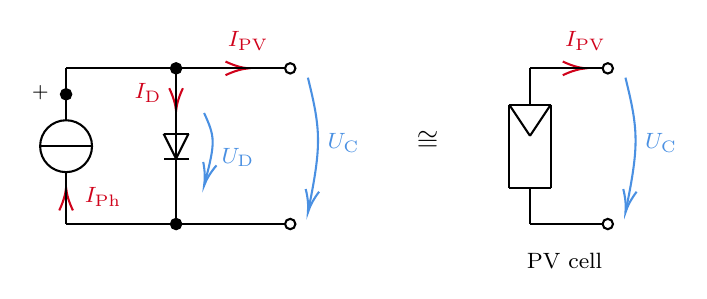
\begin{tikzpicture}[x=0.75pt,y=0.75pt,yscale=-1,xscale=1]
%uncomment if require: \path (0,391); %set diagram left start at 0, and has height of 391

%Straight Lines [id:da9220046892300695] 
\draw [color={rgb, 255:red, 208; green, 2; blue, 27 }  ,draw opacity=1 ]   (259.5,142.5) -- (273.25,142.5) ;
\draw [shift={(275.25,142.5)}, rotate = 180] [color={rgb, 255:red, 208; green, 2; blue, 27 }  ,draw opacity=1 ][line width=0.75]    (10.93,-3.29) .. controls (6.95,-1.4) and (3.31,-0.3) .. (0,0) .. controls (3.31,0.3) and (6.95,1.4) .. (10.93,3.29)   ;
%Straight Lines [id:da9695421868123493] 
\draw [color={rgb, 255:red, 208; green, 2; blue, 27 }  ,draw opacity=1 ]   (422,142.5) -- (435.75,142.5) ;
\draw [shift={(437.75,142.5)}, rotate = 180] [color={rgb, 255:red, 208; green, 2; blue, 27 }  ,draw opacity=1 ][line width=0.75]    (10.93,-3.29) .. controls (6.95,-1.4) and (3.31,-0.3) .. (0,0) .. controls (3.31,0.3) and (6.95,1.4) .. (10.93,3.29)   ;
%Straight Lines [id:da29339333794333666] 
\draw [color={rgb, 255:red, 208; green, 2; blue, 27 }  ,draw opacity=1 ]   (240.5,142.5) -- (240.5,161) ;
\draw [shift={(240.5,163)}, rotate = 270] [color={rgb, 255:red, 208; green, 2; blue, 27 }  ,draw opacity=1 ][line width=0.75]    (10.93,-3.29) .. controls (6.95,-1.4) and (3.31,-0.3) .. (0,0) .. controls (3.31,0.3) and (6.95,1.4) .. (10.93,3.29)   ;
%Straight Lines [id:da5182268392298646] 
\draw [color={rgb, 255:red, 208; green, 2; blue, 27 }  ,draw opacity=1 ]   (187.5,212.5) -- (187.5,202) ;
\draw [shift={(187.5,200)}, rotate = 450] [color={rgb, 255:red, 208; green, 2; blue, 27 }  ,draw opacity=1 ][line width=0.75]    (10.93,-3.29) .. controls (6.95,-1.4) and (3.31,-0.3) .. (0,0) .. controls (3.31,0.3) and (6.95,1.4) .. (10.93,3.29)   ;
%Straight Lines [id:da19579076658988703] 
\draw    (187.5,192.5) -- (187.5,217.5) ;
%Straight Lines [id:da500967170364542] 
\draw    (240.5,142.5) -- (240.5,217.5) ;
%Straight Lines [id:da9693092867247253] 
\draw    (187.5,142.5) -- (187.5,167.5) ;
%Straight Lines [id:da3180920793144646] 
\draw    (240.5,186) -- (234.5,186) ;
%Straight Lines [id:da3231236229149821] 
\draw    (246.5,186) -- (240.5,186) ;
%Straight Lines [id:da20274569848223778] 
\draw    (246.5,174) -- (240.5,174) ;
%Straight Lines [id:da4237476648515044] 
\draw    (240.5,174) -- (234.5,174) ;
%Straight Lines [id:da7091520922682297] 
\draw    (234.5,174) -- (240.5,186) ;
%Straight Lines [id:da8216387087718504] 
\draw    (240.5,186) -- (246.5,174) ;
%Shape: Circle [id:dp46632786849059626] 
\draw   (175,180) .. controls (175,173.1) and (180.6,167.5) .. (187.5,167.5) .. controls (194.4,167.5) and (200,173.1) .. (200,180) .. controls (200,186.9) and (194.4,192.5) .. (187.5,192.5) .. controls (180.6,192.5) and (175,186.9) .. (175,180) -- cycle ;
%Straight Lines [id:da6428722008154575] 
\draw    (175,180) -- (200,180) ;
%Shape: Circle [id:dp9143776877359857] 
\draw  [fill={rgb, 255:red, 0; green, 0; blue, 0 }  ,fill opacity=1 ] (238,217.5) .. controls (238,216.12) and (239.12,215) .. (240.5,215) .. controls (241.88,215) and (243,216.12) .. (243,217.5) .. controls (243,218.88) and (241.88,220) .. (240.5,220) .. controls (239.12,220) and (238,218.88) .. (238,217.5) -- cycle ;
%Shape: Circle [id:dp04116434903611532] 
\draw  [fill={rgb, 255:red, 0; green, 0; blue, 0 }  ,fill opacity=1 ] (185,155) .. controls (185,153.62) and (186.12,152.5) .. (187.5,152.5) .. controls (188.88,152.5) and (190,153.62) .. (190,155) .. controls (190,156.38) and (188.88,157.5) .. (187.5,157.5) .. controls (186.12,157.5) and (185,156.38) .. (185,155) -- cycle ;
%Shape: Circle [id:dp7561083964816784] 
\draw  [fill={rgb, 255:red, 0; green, 0; blue, 0 }  ,fill opacity=1 ] (238,142.5) .. controls (238,141.12) and (239.12,140) .. (240.5,140) .. controls (241.88,140) and (243,141.12) .. (243,142.5) .. controls (243,143.88) and (241.88,145) .. (240.5,145) .. controls (239.12,145) and (238,143.88) .. (238,142.5) -- cycle ;
%Curve Lines [id:da12939293693438314] 
\draw [color={rgb, 255:red, 74; green, 144; blue, 226 }  ,draw opacity=1 ]   (254,164) .. controls (259.33,175.64) and (259.5,177.87) .. (254.48,197.16) ;
\draw [shift={(254,199)}, rotate = 284.68] [color={rgb, 255:red, 74; green, 144; blue, 226 }  ,draw opacity=1 ][line width=0.75]    (10.93,-3.29) .. controls (6.95,-1.4) and (3.31,-0.3) .. (0,0) .. controls (3.31,0.3) and (6.95,1.4) .. (10.93,3.29)   ;
%Straight Lines [id:da820440930056753] 
\draw    (401,160) -- (421,160) ;
%Straight Lines [id:da5978422659023195] 
\draw    (401,160) -- (411,175) ;
%Straight Lines [id:da8646077617642114] 
\draw    (411,175) -- (421,160) ;
%Straight Lines [id:da1683854382748906] 
\draw    (401,160) -- (401,200) ;
%Straight Lines [id:da35944219412656886] 
\draw    (421,160) -- (421,200) ;
%Straight Lines [id:da012841517263090685] 
\draw    (401,200) -- (421,200) ;
%Straight Lines [id:da8937999883743217] 
\draw    (411,200) -- (411,217.5) ;
%Shape: Circle [id:dp39581519495881] 
\draw   (446,142.5) .. controls (446,141.12) and (447.12,140) .. (448.5,140) .. controls (449.88,140) and (451,141.12) .. (451,142.5) .. controls (451,143.88) and (449.88,145) .. (448.5,145) .. controls (447.12,145) and (446,143.88) .. (446,142.5) -- cycle ;
%Shape: Circle [id:dp7404102366707606] 
\draw   (446,217.5) .. controls (446,216.12) and (447.12,215) .. (448.5,215) .. controls (449.88,215) and (451,216.12) .. (451,217.5) .. controls (451,218.88) and (449.88,220) .. (448.5,220) .. controls (447.12,220) and (446,218.88) .. (446,217.5) -- cycle ;
%Straight Lines [id:da16056380159184358] 
\draw    (411,142.5) -- (446,142.5) ;
%Straight Lines [id:da8365114488683654] 
\draw    (411,217.5) -- (446,217.5) ;
%Curve Lines [id:da5511080558248806] 
\draw [color={rgb, 255:red, 74; green, 144; blue, 226 }  ,draw opacity=1 ]   (457,147) .. controls (463.37,172.48) and (463.5,179.71) .. (457.38,210.11) ;
\draw [shift={(457,212)}, rotate = 281.48] [color={rgb, 255:red, 74; green, 144; blue, 226 }  ,draw opacity=1 ][line width=0.75]    (10.93,-3.29) .. controls (6.95,-1.4) and (3.31,-0.3) .. (0,0) .. controls (3.31,0.3) and (6.95,1.4) .. (10.93,3.29)   ;
%Straight Lines [id:da725857721119765] 
\draw    (411,142.5) -- (411,160) ;
%Straight Lines [id:da5740090703572132] 
\draw    (187.5,142.5) -- (240.5,142.5) ;
%Straight Lines [id:da4778393661136311] 
\draw    (187.5,217.5) -- (240.5,217.5) ;
%Shape: Circle [id:dp2917985814178987] 
\draw   (293,142.5) .. controls (293,141.12) and (294.12,140) .. (295.5,140) .. controls (296.88,140) and (298,141.12) .. (298,142.5) .. controls (298,143.88) and (296.88,145) .. (295.5,145) .. controls (294.12,145) and (293,143.88) .. (293,142.5) -- cycle ;
%Shape: Circle [id:dp07126668235633615] 
\draw   (293,217.5) .. controls (293,216.12) and (294.12,215) .. (295.5,215) .. controls (296.88,215) and (298,216.12) .. (298,217.5) .. controls (298,218.88) and (296.88,220) .. (295.5,220) .. controls (294.12,220) and (293,218.88) .. (293,217.5) -- cycle ;
%Curve Lines [id:da8740596681425179] 
\draw [color={rgb, 255:red, 74; green, 144; blue, 226 }  ,draw opacity=1 ]   (304,147) .. controls (310.37,172.48) and (310.5,179.71) .. (304.38,210.11) ;
\draw [shift={(304,212)}, rotate = 281.48] [color={rgb, 255:red, 74; green, 144; blue, 226 }  ,draw opacity=1 ][line width=0.75]    (10.93,-3.29) .. controls (6.95,-1.4) and (3.31,-0.3) .. (0,0) .. controls (3.31,0.3) and (6.95,1.4) .. (10.93,3.29)   ;
%Straight Lines [id:da2745454915751546] 
\draw    (240.5,142.5) -- (293.5,142.5) ;
%Straight Lines [id:da3914094245668047] 
\draw    (240.5,217.5) -- (293.5,217.5) ;

% Text Node
\draw (219,148.4) node [anchor=north west][inner sep=0.75pt]  [font=\footnotesize,color={rgb, 255:red, 208; green, 2; blue, 27 }  ,opacity=1 ]  {$I_{\mathrm{D}}$};
% Text Node
\draw (195,198.4) node [anchor=north west][inner sep=0.75pt]  [font=\footnotesize,color={rgb, 255:red, 208; green, 2; blue, 27 }  ,opacity=1 ]  {$I_{\mathrm{Ph}}$};
% Text Node
\draw (261,179.4) node [anchor=north west][inner sep=0.75pt]  [font=\footnotesize,color={rgb, 255:red, 74; green, 144; blue, 226 }  ,opacity=1 ]  {$U_{\mathrm{D}}$};
% Text Node
\draw (355,171.4) node [anchor=north west][inner sep=0.75pt]  [font=\normalsize]  {$\cong $};
% Text Node
\draw (465,172.4) node [anchor=north west][inner sep=0.75pt]  [font=\footnotesize,color={rgb, 255:red, 74; green, 144; blue, 226 }  ,opacity=1 ]  {$U_{\mathrm{C}}$};
% Text Node
\draw (426.5,123.4) node [anchor=north west][inner sep=0.75pt]  [font=\footnotesize,color={rgb, 255:red, 208; green, 2; blue, 27 }  ,opacity=1 ]  {$I_{\mathrm{PV}}$};
% Text Node
\draw (408,230) node [anchor=north west][inner sep=0.75pt]  [font=\footnotesize] [align=left] {PV cell};
% Text Node
\draw (312,172.4) node [anchor=north west][inner sep=0.75pt]  [font=\footnotesize,color={rgb, 255:red, 74; green, 144; blue, 226 }  ,opacity=1 ]  {$U_{\mathrm{C}}$};
% Text Node
\draw (264,123.4) node [anchor=north west][inner sep=0.75pt]  [font=\footnotesize,color={rgb, 255:red, 208; green, 2; blue, 27 }  ,opacity=1 ]  {$I_{\mathrm{PV}}$};
% Text Node
\draw (169.5,149.4) node [anchor=north west][inner sep=0.75pt]  [font=\scriptsize]  {$+$};


\end{tikzpicture}

	\caption{Simplified standard model of a photovoltaic cell. (Recreated from: \cite{Mertens:2015, Wagner:2018})}
	\label{fig:tikz_PVC_simplified}
\end{figure}

After applying Kirchoff's first and second law to the simplified standard model, considering the equation (\ref{eq:u_pvg_sum_of_pvc}) and taking into account that the PV generator's current-voltage characteristic depends on the PV cell temperature $\vartheta_{\mathrm{C}}$ and the radiation flux $\Phi_{\mathrm{G}}$, it can be modeled with the equations (\ref{eq:i_of_u}) and (\ref{eq:u_of_i}).\footnote{Equation (\ref{eq:u_of_i}) can be derived from equations (\ref{eq:i_of_u}).}
	\begin{equation} \label{eq:i_of_u}
	\centering
		I_{\mathrm{PV}}(U_{\mathrm{PV}}, \vartheta_{\mathrm{C}}, \Phi_{\mathrm{G}}) = I_{\mathrm{Ph}} - \underbrace{I_{\mathrm{S}} \left( \exp \left(\frac{U_{\mathrm{PV}}}{m \, N_{\mathrm{C}} \, U_{\mathrm{T}} } \right) - 1  \right)}_{I_{\mathrm{D}}}
	\end{equation}
	\begin{equation} \label{eq:u_of_i}
	\centering
		U_{\mathrm{PV}}(I_{\mathrm{PV}}, \vartheta_{\mathrm{C}}, \Phi_{\mathrm{G}}) = m \, N_{\mathrm{C}} \, U_{\mathrm{T}} \, \ln \left( \frac{I_{\mathrm{Ph}} - I_{\mathrm{PV}} + I_{\mathrm{S}}}{I_{\mathrm{S}}} \right)
	\end{equation}
The diode's \emph{thermal voltage} $U_{\mathrm{T}} = U_{\mathrm{T}}(\vartheta_{\mathrm{C}})$ in $\left( \mathrm{V} \right)$, with $k_\mathrm{B} = 1,380649 \cdot 10^{-23} \mathrm{WsK^{-1}}$ being the \emph{Bolzmann constant} and $e = 1,602176634\cdot10^{-19} \mathrm{As}$ being the \emph{elementary charge}, can be obtained from the equation (\ref{eq:u_temp}).
	\begin{equation} \label{eq:u_temp}
	\centering
		U_{\mathrm{T}}(\vartheta_{\mathrm{C}}) = \frac{ k_\mathrm{B} \left( \vartheta_{\mathrm{C}} + 273,15^\circ \mathrm{C} \right) }{e} \cdot \frac{\mathrm{1K}}{1^\circ \mathrm{C}}
	\end{equation}
$m$ in $\left( 1 \right)$ is the \emph{ideality factor} with the condition $\{m \in \mathbb{R}^+ \mid 2 \geq m \geq 1 \}$. It is an empirical value that is used to model the PV cells more precisely.\footnote{For $m = 1$, $I_\mathrm{D}$ is Shockley's equation.} The quantities $I_{\mathrm{S}} = I_{\mathrm{S}}(\vartheta_{\mathrm{C}})$ in $\left( \mathrm{A} \right)$ and $I_{\mathrm{Ph}} = I_{\mathrm{Ph}}(\vartheta_{\mathrm{C}}, \Phi_{\mathrm{G}})$ in $\left( \mathrm{A} \right)$ are the diode's \emph{reverse saturation current} and the PV cell's \emph{photocurrent} \cite{Prechtl:2006, Mertens:2015, Tietze:2016, Wagner:2018, Elert:2020}. 

Based on the equation (\ref{eq:i_of_u}), the modeled current-voltage characteristic can be visualized as shown in the figure \ref{fig:tikz/tikz_PVG_curve}, where $I_{\mathrm{SC}}(\vartheta_{\mathrm{C}}, \Phi_{\mathrm{G}})$ in $\left( \mathrm{A} \right)$ and $U_{\mathrm{OC}}(\vartheta_{\mathrm{C}}, \Phi_{\mathrm{G}})$ in $\left( \mathrm{V} \right)$ are the PV generator's \emph{short-circuit current} and \emph{open-circuit voltage}. MPP is the \emph{maximum power point} for which the PV generator provides the greatest electrical power in $\left( \mathrm{W} \right)$, with $U_{\mathrm{MPP}}(\vartheta_{\mathrm{C}}, \Phi_{\mathrm{G}})$ being the voltage and $I_{\mathrm{MPP}}(\vartheta_{\mathrm{C}}, \Phi_{\mathrm{G}})$ being the current at MPP \cite{Prechtl:2006, Mertens:2015, Wagner:2018}:
	\begin{equation} \label{eq:p_mpp}
	\centering
		P_{\mathrm{MPP}}(\vartheta_{\mathrm{C}}, \Phi_{\mathrm{G}}) = U_{\mathrm{MPP}} \, I_{\mathrm{MPP}} \text{.}
	\end{equation}
\begin{figure}[h!]
	\centering
	

\tikzset{every picture/.style={line width=0.75pt}} %set default line width to 0.75pt        

\begin{tikzpicture}[x=0.75pt,y=0.75pt,yscale=-1,xscale=1]
%uncomment if require: \path (0,300); %set diagram left start at 0, and has height of 300

%Image [id:dp8816301757772553] 
\draw (309.25,160) node [xscale=-1] {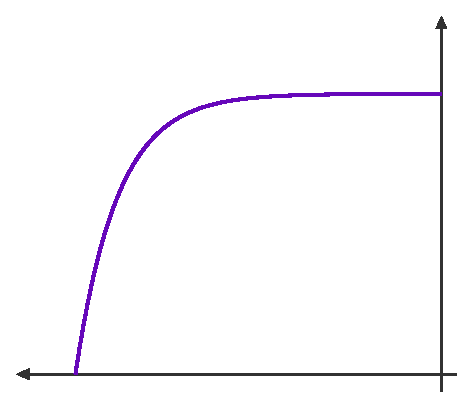
\includegraphics[width=211.13pt,height=180pt]{images/image_PVC_curve}};
%Straight Lines [id:da8531224351110531] 
\draw [color={rgb, 255:red, 155; green, 155; blue, 155 }  ,draw opacity=1 ] [dash pattern={on 4.5pt off 4.5pt}]  (184,113) -- (358,113) ;
%Straight Lines [id:da1728021335997585] 
\draw [color={rgb, 255:red, 155; green, 155; blue, 155 }  ,draw opacity=1 ] [dash pattern={on 4.5pt off 4.5pt}]  (358,113) -- (358,269) ;
%Shape: Circle [id:dp9850794530438081] 
\draw  [fill={rgb, 255:red, 255; green, 255; blue, 255 }  ,fill opacity=1 ] (356,113) .. controls (356,111.9) and (356.9,111) .. (358,111) .. controls (359.1,111) and (360,111.9) .. (360,113) .. controls (360,114.1) and (359.1,115) .. (358,115) .. controls (356.9,115) and (356,114.1) .. (356,113) -- cycle ;

% Text Node
\draw (129,19.4) node [anchor=north west][inner sep=0.75pt]  [font=\footnotesize]  {$I_{\mathrm{PV}}( U_{\mathrm{PV}} ,\vartheta _{\mathrm{C}} ,\Phi _{\mathrm{G}})$};
% Text Node
\draw (456,263.4) node [anchor=north west][inner sep=0.75pt]  [font=\footnotesize]  {$U_{\mathrm{PV}}$};
% Text Node
\draw (278,276.4) node [anchor=north west][inner sep=0.75pt]  [font=\footnotesize]  {$U_{\mathrm{MPP}}( \vartheta _{\mathrm{C}} ,\Phi _{\mathrm{G}})$};
% Text Node
\draw (91,105.4) node [anchor=north west][inner sep=0.75pt]  [font=\footnotesize]  {$I_{\mathrm{MPP}}( \vartheta _{\mathrm{C}} ,\Phi _{\mathrm{G}})$};
% Text Node
\draw (361,96) node [anchor=north west][inner sep=0.75pt]  [font=\footnotesize] [align=left] {MPP};
% Text Node
\draw (370,276.4) node [anchor=north west][inner sep=0.75pt]  [font=\footnotesize]  {$U_{\mathrm{OC}}( \vartheta _{\mathrm{C}} ,\Phi _{\mathrm{G}})$};
% Text Node
\draw (102,83.4) node [anchor=north west][inner sep=0.75pt]  [font=\footnotesize]  {$I_{\mathrm{SC}}( \vartheta _{\mathrm{C}} ,\Phi _{\mathrm{G}})$};
% Text Node
\draw (166,273.4) node [anchor=north west][inner sep=0.75pt]  [font=\footnotesize]  {$0$};


\end{tikzpicture}


	\caption{Modeled current-voltage characteristic of a photovoltaic generator, depending on the radiation flux $\Phi_{\mathrm{G}}$ and the photovoltaic cell temperature $\vartheta_{\mathrm{C}}$. (Recreated from: \cite{Mertens:2015, Wagner:2018})}
	\label{fig:tikz/tikz_PVG_curve}
\end{figure}

The quantity in the simplified standard model that changes with the solar radiation is the photocurrent. It is proportional to the radiation flux $\Phi_{\mathrm{G}}$, with $S = \mathrm{const.}$ in $\left( \mathrm{A}\mathrm{W^{-1}} \right)$ being the \emph{sensitivity} of the PV cell:
	\begin{equation} \label{eq:photo_i}
	\centering
		I_{\mathrm{Ph}}(\vartheta_{\mathrm{STC}}, \Phi_{\mathrm{G}}) = S \, \Phi_{\mathrm{G}} \text{.}
	\end{equation}
From the case $I_{\mathrm{PV}}(0\mathrm{V}, \vartheta_{\mathrm{STC}}, \Phi_{\mathrm{STC}}) = I_\mathrm{SC,STC}$, the sensitivity can be obtained as shown in the equation (\ref{eq:sens}).
	\begin{equation} \label{eq:sens}
	\centering
		 S = \frac{I_\mathrm{SC,STC}}{\Phi_{\mathrm{STC}}}
	\end{equation}
For the \emph{standard test conditions} (STC), listed in the table \ref{tab:table_STC}, $I_\mathrm{SC,STC}$ can be taken directly from the data sheet of a PV generator and $\Phi_{\mathrm{STC}}$ in $\left( \mathrm{W} \right)$ can be calculated using the equation (\ref{eq:radiation_flux}). In this equation, $A_\mathrm{PV}$ can either be measured or taken from a PV generator's data sheet as well.
\begin{table}[h!]
	\centering
	\footnotesize
\begin{tabular}{|l|c|}
	\hline
	\multicolumn{2}{|c|}{\textbf{Standard test conditions for PV generators}} \\
	\hline
 	Total irradiance received by the PV generator & $E_{\mathrm{STC}} = 1000\mathrm{W} \mathrm{m}^{-2}$ \\
	PV cell temperature & $\vartheta_{\mathrm{STC}} = 25^\circ \mathrm{C}$ \\
	Solar spectrum & AM 1,5 \\
	\hline
\end{tabular}
	\caption{Parameters for the standard test conditions of a photovoltaic generator \cite{Mertens:2015}.}
	\label{tab:table_STC}
\end{table}
After substituting equation (\ref{eq:sens}) into equation (\ref{eq:photo_i}) and taking the \emph{temperature coefficient} of the short circuit current $\mathrm{TC}(I_{\mathrm{SC}})$ in $\left( \% ^\circ \mathrm{C}^{-1} \right)$ into account, the photocurrent, depending on the PV cell temperature and the radiation flux, follows to:
	\begin{equation} \label{eq:i_ph_theta_phi}
	\centering
		 I_{\mathrm{Ph}}(\vartheta_{\mathrm{C}}, \Phi_{\mathrm{G}}) = \underbrace{I_{\mathrm{SC,STC}} \, \frac{E_\mathrm{G}}{E_\mathrm{STC}}}_{I_{\mathrm{Ph}}(\vartheta_{\mathrm{STC}}, \Phi_{\mathrm{G}})} \left[ 1 + \frac{\mathrm{TC}(I_{\mathrm{SC}})}{100\%} \left(\vartheta_{\mathrm{C}} - \vartheta_{\mathrm{STC}} \right) \right] \text{.}
	\end{equation}
$\mathrm{TC}(I_{\mathrm{SC}})$ can usually be taken from a PV generator's data sheet.\footnote{Typical $\mathrm{TC}(I_{\mathrm{SC}})$ values for Si-PV cells are around $0,06 \% ^\circ \mathrm{C}^{-1}$.} Because $I_{\mathrm{PV}}(0\mathrm{V}, \vartheta_{\mathrm{C}}, \Phi_{\mathrm{G}}) = I_{\mathrm{SC}}(\vartheta_{\mathrm{C}}, \Phi_{\mathrm{G}})$, $I_{\mathrm{SC}}(\vartheta_{\mathrm{C}}, \Phi_{\mathrm{G}}) = I_{\mathrm{Ph}}(\vartheta_{\mathrm{C}}, \Phi_{\mathrm{G}})$ applies \cite{Mertens:2015, Tietze:2016, Wagner:2018}. 

Now that $I_{\mathrm{Ph}}(\vartheta_{\mathrm{C}}, \Phi_{\mathrm{G}})$ is known, the diode's reverse saturation current can be calculated from the case $I_{\mathrm{PV}}\big(U_{\mathrm{OC}}(\vartheta_{\mathrm{C}}, \Phi_{\mathrm{G}}), \vartheta_{\mathrm{C}}, \Phi_{\mathrm{G}}\big) = 0\mathrm{A}$: 
	\begin{equation} \label{eq:I_S_theta_phi}
	\centering
		I_\mathrm{S}(\vartheta_{\mathrm{C}}) = I_{\mathrm{Ph}}( \vartheta_{\mathrm{C}}, \Phi_{\mathrm{G}}) \left( \exp \left( \frac{U_\mathrm{OC}(\vartheta_{\mathrm{C}}, \Phi_{\mathrm{G}})}{m \, N_\mathrm{C} \, U_\mathrm{T}} \right) - 1 \right)^{-1} \text{.}
	\end{equation}
The open-circuit voltage $U_\mathrm{OC}(\vartheta_{\mathrm{C}}, \Phi_{\mathrm{G}})$ can be derived by subtracting the case $U_{\mathrm{PV}}( 0\mathrm{A}, \vartheta_{\mathrm{C}}, \Phi_{\mathrm{G}})$ from the case $U_{\mathrm{PV}}(0\mathrm{A}, \vartheta_{\mathrm{C}}, \Phi_{\mathrm{STC}})$ while taking the temperature coefficient of the open-circuit voltage $\mathrm{TC}(U_{\mathrm{OC}})$ in $\left( \% ^\circ \mathrm{C}^{-1} \right)$ into account:
	\begin{equation} \label{eq:U_OC_theta_phi}
	\centering
		U_\mathrm{OC}(\vartheta_{\mathrm{C}}, \Phi_{\mathrm{G}}) = U_\mathrm{OC}(\vartheta_{\mathrm{C}},\Phi_\mathrm{STC}) + m \, N_\mathrm{C} \, U_\mathrm{T} \, \ln \left( \frac{I_{\mathrm{Ph}}(\vartheta_{\mathrm{C}}, \Phi_{\mathrm{G}}) + I_{\mathrm{S}}(\vartheta_{\mathrm{C}})}{I_\mathrm{Ph}(\vartheta_{\mathrm{C}},\Phi_\mathrm{STC}) + I_{\mathrm{S}}( \vartheta_{\mathrm{C}})} \right) \text{,}
	\end{equation}
where $U_\mathrm{OC}(\vartheta_{\mathrm{C}},\Phi_\mathrm{STC})$ is the temperature dependent open-circuit voltage for the radiation flux $\Phi_\mathrm{STC}$ at STC: 
	\begin{equation} \label{eq:U_OC_phi_STC}
	\centering
		U_\mathrm{OC}(\vartheta_{\mathrm{C}},\Phi_\mathrm{STC}) = U_\mathrm{OC,STC} \left[ 1 + \frac{\mathrm{TC}(U_{\mathrm{OC}})}{100\%} \left(\vartheta_{\mathrm{C}} - \vartheta_{\mathrm{STC}} \right) \right] \text{.}
	\end{equation}
In addition to $\mathrm{TC}(I_{\mathrm{SC}})$, $\mathrm{TC}(U_{\mathrm{OC}})$ can also be taken from a PV generators data sheet.\footnote{Typical $\mathrm{TC}(U_{\mathrm{OC}})$ values for Si-PV cells are around $-0,40 \% ^\circ \mathrm{C}^{-1}$.} Equation (\ref{eq:U_OC_theta_phi}) is only valid because the reverse saturation current $I_\mathrm{S}(\vartheta_{\mathrm{C}})$ does not depend on the radiation flux \cite{Mertens:2015, Tietze:2016, Hering:2017, Wagner:2018}. 

Since the equations (\ref{eq:I_S_theta_phi}) and (\ref{eq:U_OC_theta_phi}) are in a non-linear relationship to one another, the Newton-Raphson method must be used to approximate them numerically (see appendix \ref{sec:newton_raphson_method}). For this, the functions $f_1(\mathrm{\mathbf{x}}_R)$ and $f_2(\mathrm{\mathbf{x}}_R)$ are introduced below. In the equation (\ref{eq:f_1}) an exponential function is used instead of a logarthmic function, since some numerical approximation algorithms do not converge for logarithmic functions.
	\begin{equation} \label{eq:f_1}
	\centering
		\begin{split}
		f_1(\mathrm{\mathbf{x}}_R) = \exp \left( \frac{U_\mathrm{OC}(\vartheta_{\mathrm{C}}, \Phi_{\mathrm{G}}) - U_\mathrm{OC}(\vartheta_{\mathrm{C}},\Phi_\mathrm{STC})}{m \, N_\mathrm{C} \, U_\mathrm{T}} \right) \\ - \frac{I_{\mathrm{Ph}}(\vartheta_{\mathrm{C}}, \Phi_{\mathrm{G}}) + I_{\mathrm{S}}(\vartheta_{\mathrm{C}})}{I_\mathrm{Ph}(\vartheta_{\mathrm{C}},\Phi_\mathrm{STC}) + I_{\mathrm{S}}(\vartheta_{\mathrm{C}})} = 0
		\end{split}
	\end{equation}
	\begin{equation} \label{eq:f_2}
	\centering
		f_2(\mathrm{\mathbf{x}}_R) = I_\mathrm{S}(\vartheta_{\mathrm{C}}) - I_\mathrm{Ph}(\vartheta_{\mathrm{C}}, \Phi_{\mathrm{G}}) \left(\exp \left(\frac{U_\mathrm{OC}(\vartheta_{\mathrm{C}}, \Phi_{\mathrm{G}})}{m \, N_\mathrm{C} \, U_\mathrm{T}} \right) - 1 \right)^{-1} = 0\mathrm{A}
	\end{equation}
The vector $\mathrm{\mathbf{x}}_R$, shown in the equation (\ref{eq:x_r_vector}), contains the zero crossings of the functions $f_1(\mathrm{\mathbf{x}}_R)$ and $f_2(\mathrm{\mathbf{x}}_R)$. 
	\begin{equation} \label{eq:x_r_vector}
	\centering
		\mathrm{\mathbf{x}}_R = \Big( I_\mathrm{S}(\vartheta_{\mathrm{C}}), U_\mathrm{OC}(\vartheta_{\mathrm{C}}, \Phi_{\mathrm{G}}) \Big)^{\mathrm T}
	\end{equation}
Furthermore, the vector $\mathrm{\mathbf{f}}(\mathrm{\mathbf{x}}_R) = \mathbf{0}$, which contains the functions from the equations (\ref{eq:f_1}) and (\ref{eq:f_2}), must be introduced for the Newton-Raphson method:
	\begin{equation} \label{eq:f_vector}
	\centering
		\mathrm{\mathbf{f}}(\mathrm{\mathbf{x}}_R) = 
  			\Big( f_{1}(\mathrm{\mathbf{x}}_R), f_{2}(\mathrm{\mathbf{x}}_R) \Big)^{\mathrm T} = \mathrm{\mathbf{0}} \text{.}
	\end{equation}
With the help of the Jacobian matrix $\mathrm{\mathbf{J}} = \partial \mathrm{\mathbf{f}}(\mathrm{\mathbf{x}}) / \partial \mathrm{\mathbf{x}}$ for $\mathrm{\mathbf{x}} = \mathrm{\mathbf{x}}_R$, the $\left(n + 1\right)$\textsuperscript{th} approximation with $n \in \mathbb{N}$ can be determined as follows:
	\begin{equation} \label{eq:vect_U_I_approx}
	\centering
		\mathrm{\mathbf{x}}_{R, n + 1} = \mathrm{\mathbf{x}}_{R,n} 	- \mathrm{\mathbf{J}}^{-1}(\mathrm{\mathbf{x}}_{R,n}) \, \mathrm{\mathbf{f}}(\mathrm{\mathbf{x}}_{R,n}) \text{,}
	\end{equation}
	\begin{equation} \label{eq:jacobian_for_PVG}
	\centering
		\mathrm{\mathbf{J}} =  
 		\begin{pmatrix}
  			\dfrac{\partial f_1\big( I_\mathrm{S}(\vartheta_{\mathrm{C}}), U_\mathrm{OC}(\vartheta_{\mathrm{C}},\Phi_{\mathrm{G}}) \big)}{\partial I_\mathrm{S}(\vartheta_{\mathrm{C}})}  & \dfrac{\partial  f_1\big( I_\mathrm{S}(\vartheta_{\mathrm{C}}), U_\mathrm{OC}(\vartheta_{\mathrm{C}},\Phi_{\mathrm{G}}) \big)}{\partial U_\mathrm{OC}(\vartheta_{\mathrm{C}},\Phi_{\mathrm{G}})} \\
			\dfrac{\partial f_2\big( I_\mathrm{S}(\vartheta_{\mathrm{C}}), U_\mathrm{OC}(\vartheta_{\mathrm{C}},\Phi_{\mathrm{G}}) \big)}{\partial I_\mathrm{S}(\vartheta_{\mathrm{C}})} & \dfrac{\partial f_2\big( I_\mathrm{S}(\vartheta_{\mathrm{C}}), U_\mathrm{OC}(\vartheta_{\mathrm{C}},\Phi_{\mathrm{G}}) \big)}{\partial U_\mathrm{OC}(\vartheta_{\mathrm{C}},\Phi_{\mathrm{G}})} 
 		\end{pmatrix} \text{.}
 	\end{equation}
Starting values for the Newton-Raphson method can be obtained from the expressions in the equation (\ref{eq:U_OC_I_S_zero}), if it is accepted that the diode's reverse saturation current $I_{\mathrm{S}}$ is small compared to the photocurrent $I_{\mathrm{Ph}}$, so that $I_{\mathrm{S}} + I_{\mathrm{Ph}} \approx I_{\mathrm{Ph}}$ applies.\footnote{These expressions can be derived from the equations (\ref{eq:U_OC_theta_phi}) and (\ref{eq:I_S_theta_phi}).}
	\begin{equation} \label{eq:U_OC_I_S_zero}
	\centering
		\begin{gathered}
		 U_{\mathrm{OC,0}}(\vartheta_{\mathrm{C}}, \Phi_{\mathrm{G}}) = U_\mathrm{OC}(\vartheta_{\mathrm{C}},\Phi_\mathrm{STC}) + m \, N_\mathrm{C} \, U_\mathrm{T} \, \ln \left( \frac{I_\mathrm{Ph}(\vartheta_{\mathrm{C}}, \Phi_{\mathrm{G}})}{I_\mathrm{Ph}(\vartheta_{\mathrm{C}},\Phi_\mathrm{STC})} \right)\text{,} \\
		 I_\mathrm{S,0}(\vartheta_{\mathrm{C}}) = I_{\mathrm{Ph}}(\vartheta_{\mathrm{C}}, \Phi_{\mathrm{G}}) \, \exp \left( - \frac{U_\mathrm{OC,0}(\vartheta_{\mathrm{C}}, \Phi_{\mathrm{G}})}{m \, N_\mathrm{C} \, U_\mathrm{T}} \right)\text{,} \\ \text{for } I_\mathrm{S} \ll I_\mathrm{Ph}
		 \end{gathered}
	\end{equation}
With these, the starting vector $\mathrm{\mathbf{x}}_{R,0} = \big( I_\mathrm{S,0}(\vartheta_{\mathrm{C}}), U_\mathrm{OC,0}(\vartheta_{\mathrm{C}}, \Phi_{\mathrm{G}}) \big)^{\mathrm T}$ for the first iteration can be obtained. Finally, it has to mentioned that the functions $f_1(\mathrm{\mathbf{x}}_R)$ and $f_2(\mathrm{\mathbf{x}}_R)$ are continuously differentiable for the required number of iteration steps $n + 1$. This is a requirement for the Newton-Raphson method \cite{Schwarz:2011, Rudolf:2014, Taschner:2014, Mertens:2015, Wagner:2018, Kugi:2021}.

The PV cell temperature $\vartheta_{\mathrm{C}}$, depending on the irradiance $E_{\mathrm{G}}$ and the \emph{ambient temperature} $\vartheta_{\mathrm{A}}$ in $\left( ^\circ \mathrm{C} \right)$, with the \emph{nominal operating cell temperature}\footnote{Typical $\mathrm{NOCT}$ values for c-Si-PV generators are around $45$ to $50^\circ \mathrm{C}$.} $\mathrm{NOCT}$ in $\left( ^\circ \mathrm{C} \right)$ and the conditions under which it is measured, $\vartheta_{\mathrm{A,NOCT}}$ in $\left( ^\circ \mathrm{C} \right)$ and $E_{\mathrm{NOCT}}$ in $\left( \mathrm{W} \mathrm{m}^{-2} \right)$, can be approximated by assuming that the increase of $\vartheta_{\mathrm{C}}$, compared to the ambient temperature $\vartheta_{\mathrm{A}}$, is proportional to $E_{\mathrm{G}}$:
	\begin{equation} \label{eq:cell_temp}
	\centering
		\vartheta_{\mathrm{C}} \approx \vartheta_{\mathrm{A}} + \left(\mathrm{NOCT} - \vartheta_{\mathrm{A,NOCT}}\right) \frac{E_{\mathrm{G}}}{E_{\mathrm{NOCT}}} \text{.}
	\end{equation}
The paramateres under which the $\mathrm{NOCT}$ is measured are provided by the table \ref{tab:table_NOCT} and the $\mathrm{NOCT}$ is usually listed in the data sheet of a PV generator \cite{Mertens:2015}.
\begin{table}[h!]
	\centering
	\footnotesize
\begin{tabular}{|l|c|}
	\hline
	\multicolumn{2}{|c|}{\textbf{Conditions for NOCT measurement}} \\
	\hline
 	Total irradiance received by the PV generator & $E_{\mathrm{NOCT}} = 800\mathrm{W} \mathrm{m}^{-2}$ \\
	Ambient temperature & $\vartheta_{\mathrm{A, NOCT}} = 20^\circ \mathrm{C}$ \\
	Wind speed & $v_{\mathrm W} = 1 \mathrm{m} \mathrm{s}^{-1}$  \\
	\hline
\end{tabular}
	\caption{Conditions under which the NOCT is measured \cite{Mertens:2015}.}
	\label{tab:table_NOCT}
\end{table}

Ambient temperatures $\vartheta_{\mathrm{A}}$ for different locations on Earth can be obtained from climate charts. For example, figure \ref{fig:temp_vienna} presents monthly averages for the ambient temperature in $\left( ^\circ \mathrm{C} \right)$ and precipitation in $\left( \mathrm{mm} \right)$ collected by the Global Historical Climatology Network for the Hohe Warte in Vienna, Austria, between 1997 and 2016. Below the chart, the percentage of missing data regarding the months of the year is presented \cite{Zepner:2020}.
\begin{figure}[h!]
	\centering
  	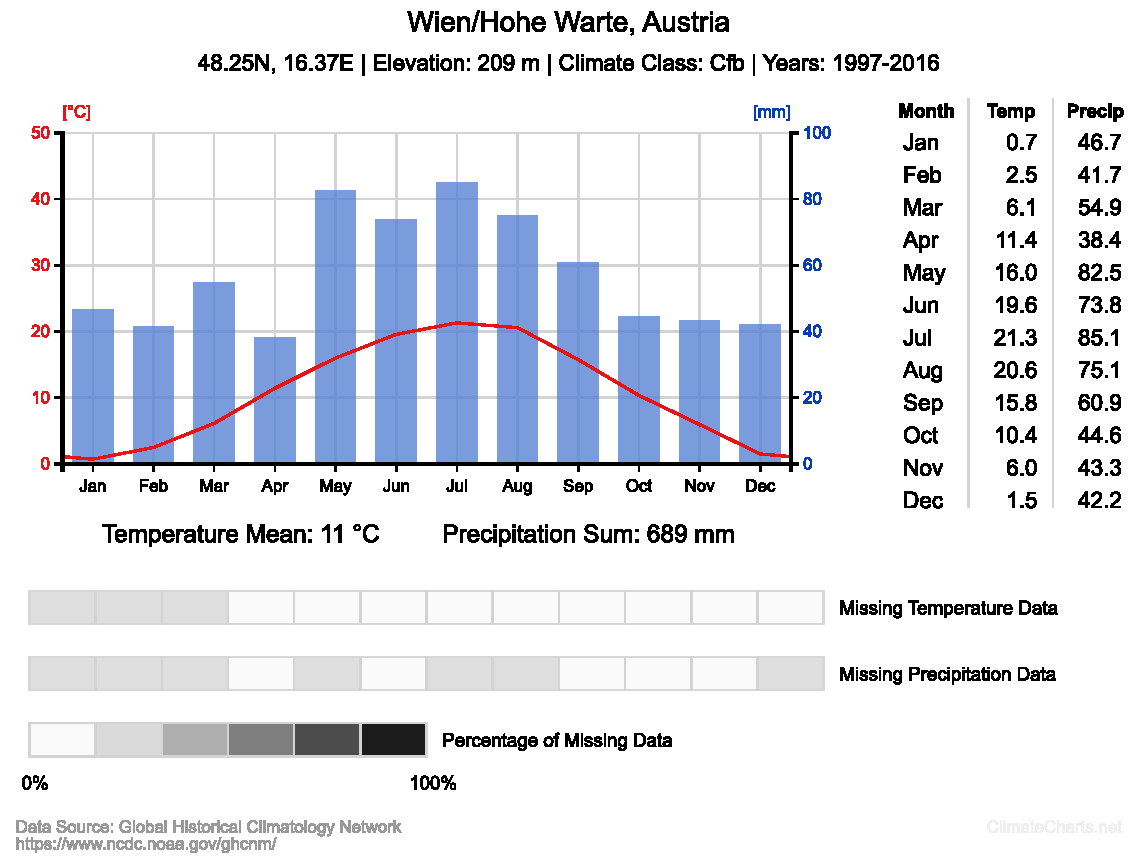
\includegraphics[width = 0.96\textwidth]{temp_maps/temp_vienna}
  	\caption{Monthly averages of temperature and precipitation data for the Hohe Warte in Vienna, Austria. (Image credit: \cite{Zepner:2020})}
	\label{fig:temp_vienna}
\end{figure}

Building on the previous findings, the electrical power output of a PV generator can be calculted by using one of the following equations:
	\begin{equation} \label{eq:p_pv_i}
	\centering
		P_{\mathrm{PV}}(I_{\mathrm{PV}}, \vartheta_{\mathrm{C}}, \Phi_{\mathrm{G}}) = m \, N_{\mathrm{C}} \, U_{\mathrm{T}} \, I_{\mathrm{PV}} \, \ln \left( \frac{I_{\mathrm{Ph}} - I_{\mathrm{PV}} + I_{\mathrm{S}}}{I_{\mathrm{S}}} \right) \text{,}
	\end{equation}
	\begin{equation} \label{eq:p_pv_u}
	\centering
		 P_{\mathrm{PV}}(U_{\mathrm{PV}}, \vartheta_{\mathrm{C}}, \Phi_{\mathrm{G}}) = U_{\mathrm{PV}} \left[ I_{\mathrm{Ph}} - I_{\mathrm{S}} \left( \exp \left(\frac{U_{\mathrm{PV}}}{m \, N_{\mathrm{C}} \, U_{\mathrm{T}} } \right) - 1  \right) \right] \text{.}
	\end{equation}
Typically, $P_{\mathrm{PV}}$ is plotted as a function of $U_{\mathrm{PV}}$, which results in a curve as shown in the figure \ref{fig:tikz_PVG_power_curve} \cite{Prechtl:2006, Mertens:2015, Wagner:2018}.
\begin{figure}[h!]
	\centering
	

\tikzset{every picture/.style={line width=0.75pt}} %set default line width to 0.75pt        

\begin{tikzpicture}[x=0.75pt,y=0.75pt,yscale=-1,xscale=1]
%uncomment if require: \path (0,425); %set diagram left start at 0, and has height of 425

%Image [id:dp09113935256135308] 
\draw (346,215.5) node  {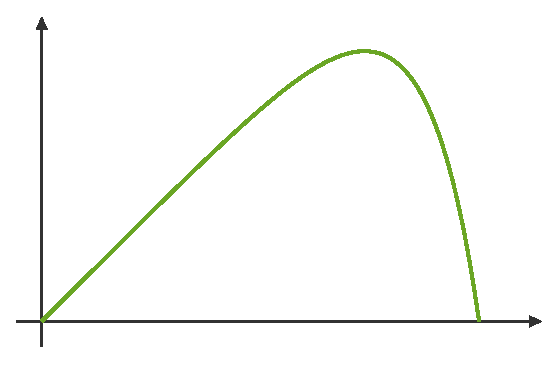
\includegraphics[width=252pt,height=158.25pt]{image_PVG_power_curve}};
%Straight Lines [id:da17852705755040943] 
\draw [color={rgb, 255:red, 155; green, 155; blue, 155 }  ,draw opacity=1 ] [dash pattern={on 4.5pt off 4.5pt}]  (199,132) -- (386,132) ;
%Straight Lines [id:da5125910827691256] 
\draw [color={rgb, 255:red, 155; green, 155; blue, 155 }  ,draw opacity=1 ] [dash pattern={on 4.5pt off 4.5pt}]  (401,138) -- (401,304) ;
%Shape: Circle [id:dp819738962444466] 
\draw  [fill={rgb, 255:red, 255; green, 255; blue, 255 }  ,fill opacity=1 ] (399,132) .. controls (399,130.9) and (399.9,130) .. (401,130) .. controls (402.1,130) and (403,130.9) .. (403,132) .. controls (403,133.1) and (402.1,134) .. (401,134) .. controls (399.9,134) and (399,133.1) .. (399,132) -- cycle ;

% Text Node
\draw (103,123.4) node [anchor=north west][inner sep=0.75pt]  [font=\footnotesize]  {$P_{\mathrm{MPP}}( \vartheta _{\mathrm{C}} ,\Phi _{\mathrm{G}})$};
% Text Node
\draw (334.71,308.4) node [anchor=north west][inner sep=0.75pt]  [font=\footnotesize]  {$U_{\mathrm{MPP}}( \vartheta _{\mathrm{C}} ,\Phi _{\mathrm{G}})$};
% Text Node
\draw (520,298.4) node [anchor=north west][inner sep=0.75pt]  [font=\footnotesize]  {$U_{\mathrm{PV}}$};
% Text Node
\draw (139,89.4) node [anchor=north west][inner sep=0.75pt]  [font=\footnotesize]  {$P_{\mathrm{PV}}( U_{\mathrm{PV}} ,\vartheta _{\mathrm{C}} ,\Phi _{\mathrm{G}})$};
% Text Node
\draw (384.5,112) node [anchor=north west][inner sep=0.75pt]  [font=\footnotesize] [align=left] {MPP};
% Text Node
\draw (427.86,308.4) node [anchor=north west][inner sep=0.75pt]  [font=\footnotesize]  {$U_{\mathrm{OC}}( \vartheta _{\mathrm{C}} ,\Phi _{\mathrm{G}})$};
% Text Node
\draw (180,308.4) node [anchor=north west][inner sep=0.75pt]  [font=\footnotesize]  {$0$};


\end{tikzpicture}

	\caption{Electrical power output of a photovoltaic generator as a function of $U_{\mathrm{PV}}$. It is further dependent on the photovoltaic cell temperature $\vartheta_{\mathrm{C}}$ and the radiation flux $\Phi_{\mathrm{G}}$. (Recreated from: \cite{Mertens:2015})}
	\label{fig:tikz_PVG_power_curve}
\end{figure}
\subsection{MPP tracking solar charging controllers}
The aim of a SCC is to distribute a PV generator's electrical energy to supply one or more electrical consumers and to recharge an electrochemical energy storage device. The latter is required to supply electrical consumers during times without sunlight. SCCs that can track the MPP of a PV generator, thus providing the greatest electrical energy to the load and the electrochemical energy storage device (compare to figure \ref{fig:tikz/tikz_solar_energy_distribution}), determine the current $I_{\mathrm{MPP}}(\vartheta_{\mathrm{C}}, \Phi_{\mathrm{G}})$ and voltage $U_{\mathrm{MPP}}(\vartheta_{\mathrm{C}}, \Phi_{\mathrm{G}})$. This can be accomplished by analyzing the equation (\ref{eq:p_pv_i}) from which the derivative of $P_{\mathrm{PV}}(I_{\mathrm{PV}}, \vartheta_{\mathrm{C}}, \Phi_{\mathrm{G}})$, with respect to $I_{\mathrm{PV}}$, results in the equation (\ref{eq:dp_pv}).
	\begin{equation} \label{eq:dp_pv}
	\centering
		 \dfrac{\mathrm d P_{\mathrm{PV}}(I_{\mathrm{PV}}, \vartheta_{\mathrm{C}}, \Phi_{\mathrm{G}})}{\mathrm d I_{\mathrm{PV}}} = m \, N_{\mathrm{C}} \, U_{\mathrm{T}} \left( \ln \left( \frac{I_{\mathrm{Ph}} - I_{\mathrm{PV}} + I_{\mathrm{S}}}{I_{\mathrm{S}}} \right) - \frac{I_{\mathrm{PV}}}{I_{\mathrm{Ph}} - I_{\mathrm{PV}} + I_{\mathrm{S}}} \right)
	\end{equation}
Since the slope of the curve $P_{\mathrm{PV}}(I_{\mathrm{PV}}, \vartheta_{\mathrm{C}}, \Phi_{\mathrm{G}})$ becomes $0\mathrm{V}$ for its maxima, $I_{\mathrm{PV}} = I_{\mathrm{MPP}}$ applies as shown below:
	\begin{equation} \label{eq:dp_pv_zero}
	\centering
		 m \, N_{\mathrm{C}} \, U_{\mathrm{T}} \left( \ln \left( \frac{I_{\mathrm{Ph}} - I_{\mathrm{MPP}} + I_{\mathrm{S}}}{I_{\mathrm{S}}} \right) - \frac{I_{\mathrm{MPP}}}{I_{\mathrm{Ph}} - I_{\mathrm{PV}} + I_{\mathrm{S}}} \right) = 0\mathrm{V} \text{.}
	\end{equation}
If now the equation (\ref{eq:dp_pv_zero}) is subtracted from the equation (\ref{eq:u_of_i}) for the case $U_{\mathrm{PV}}(I_{\mathrm{MPP}}, \vartheta_{\mathrm{C}}, \Phi_{\mathrm{G}}) = U_{\mathrm{MPP}}(\vartheta_{\mathrm{C}}, \Phi_{\mathrm{G}})$, the voltage at MPP can be rewritten as follows \cite{Mertens:2015, Wagner:2018}:
	\begin{equation} \label{eq:u_mpp_i_mpp}
	\centering
		 U_{\mathrm{MPP}}(I_{\mathrm{MPP}}, \vartheta_{\mathrm{C}}, \Phi_{\mathrm{G}}) = \frac{m \, N_{\mathrm{C}} \, U_{\mathrm{T}} \, I_{\mathrm{MPP}}}{I_{\mathrm{Ph}} - I_{\mathrm{MPP}} + I_{\mathrm{S}}} \text{.}
	\end{equation}

In addition to the equation (\ref{eq:p_mpp}), $P_{\mathrm{MPP}}(\vartheta_{\mathrm{C}}, \Phi_{\mathrm{G}})$ can directly be obtained from $\Phi_{\mathrm G}$ as presented in the equation (\ref{eq:p_mpp_phi_temp}). For this, however, the PV generator's \emph{efficiency} $\eta_{\mathrm{PV}}$ in $\left(1\right)$ and its temperature coefficient $\mathrm{TC}(P_{\mathrm{MPP}})$ in $\left( \% ^\circ \mathrm{C}^{-1}\right)$ for the electrical power output at MPP must be known.\footnote{Typical $\mathrm{TC}(P_{\mathrm{MPP}})$ values for Si-PV cells are around $-0,4$ to $-0,5$ $\% ^\circ \mathrm{C}^{-1}$.} These quantities can be found in the data sheet of a PV generator. 
	\begin{equation} \label{eq:p_mpp_phi_temp}
	\centering
		 P_{\mathrm{MPP}}(\vartheta_{\mathrm{C}}, \Phi_{\mathrm{G}}) = \eta_{\mathrm{PV}} \, \Phi_{\mathrm G} \left[ 1 + \frac{\mathrm{TC}(P_{\mathrm{MPP}})}{100\%} \left(\vartheta_{\mathrm{C}} - \vartheta_{\mathrm{STC}} \right) \right]
	\end{equation}
Alternatively, $\eta_{\mathrm{PV}}$ can be calculated by using the equation (\ref{eq:p_mpp_phi_temp}) and the table \ref{tab:table_STC}, while regarding the expression $P_\mathrm{MPP,STC} = U_\mathrm{MPP,STC} \, I_\mathrm{MPP,STC}$. This is because $\eta_{\mathrm{PV}}$ depends exclusively on the material and the structure of a PV cell. Moreover, it is assumed that the PV cell is ideal and that every photon which hits the semiconductor and fulfills $W_{\mathrm{Ph}} > \Delta W_{\mathrm{gap}}$, is absorbed and leads to an electron which contributes to $I_\mathrm{Ph}$. In the mentioned inequality $W_{\mathrm{Ph}}$ is the \emph{energy of a photon} in $\left(\mathrm{eV}\right)$ and $\Delta W_{\mathrm{gap}}$ is the \emph{band gap} in $\left(\mathrm{eV}\right)$ of the semiconductor \cite{Mertens:2015, Wagner:2018}.

With the equations (\ref{eq:p_mpp}), (\ref{eq:u_mpp_i_mpp}) and (\ref{eq:p_mpp_phi_temp}), the PV generator's current at MPP can be converted into the following quadratic equation:
	\begin{equation} \label{eq:i_mpp_quadratic}
	\centering
		 I_{\mathrm{MPP}}^2 + c_{\mathrm{PV}} \, I_{\mathrm{MPP}} - c_{\mathrm{PV}} \left(I_{\mathrm{Ph}} + I_{\mathrm{S}}\right) = 0\mathrm{A}^2 \text{, }
	\end{equation}
with $c_{\mathrm{PV}}$ being:
	\begin{equation} \label{eq:c_pv}
	\centering
		 c_{\mathrm{PV}} = \dfrac{\eta_{\mathrm{PV}} \, \Phi_{\mathrm G} \left[ 1 + \dfrac{\mathrm{TC}(P_{\mathrm{MPP}})}{100\%} \left(\vartheta_{\mathrm{C}} - \vartheta_{\mathrm{STC}} \right) \right]}{m \, N_{\mathrm{C}} \, U_{\mathrm{T}}} \text{.}
	\end{equation}
Finally, $I_{\mathrm{MPP}}(\vartheta_{\mathrm{C}}, \Phi_{\mathrm{G}})$ can be solved to:
	\begin{equation} \label{eq:i_mpp_sqr_root}
	\centering
		 I_{\mathrm{MPP}}(\vartheta_{\mathrm{C}}, \Phi_{\mathrm{G}}) = \sqrt{\frac{c_{\mathrm{PV}}^2}{4} + c_{\mathrm{PV}} \left(I_{\mathrm{Ph}} + I_{\mathrm{S}}\right)} - \frac{c_{\mathrm{PV}}}{2} \text{.}
	\end{equation}
The PV generator's voltage at MPP can consequently be calculated using the equation (\ref{eq:i_of_u}) for the case $U_{\mathrm{PV}}(I_{\mathrm{MPP}}, \vartheta_{\mathrm{C}}, \Phi_{\mathrm{G}})$, or using the equation (\ref{eq:u_mpp_i_mpp}).

Due to the fact that real MPP tracking SCCs do not have information about the connected PV generator, a \emph{shunt resistor} $R_\mathrm{shunt}$ in $\left( \Omega \right)$ is used to find the MPP. A charging- and MPP-controller inside the SCC then controls the \emph{duty cycle} $a$ in $\left( \% \right)$ of a DC/DC converter, so that the load and the electrochemical energy storage device are supplied with the greatest electrical energy. An illustration of the basic structure of such a MPP tracking SCC can be seen in the figure \ref{fig:tikz_SCC}. $I_\mathrm{SCC}$ in $\left(\mathrm{A}\right)$ is the current that is consumed by the charging- and MPP-controller \cite{Mertens:2015}. 
\begin{figure}[h!]
	\centering
	

\tikzset{every picture/.style={line width=0.75pt}} %set default line width to 0.75pt        

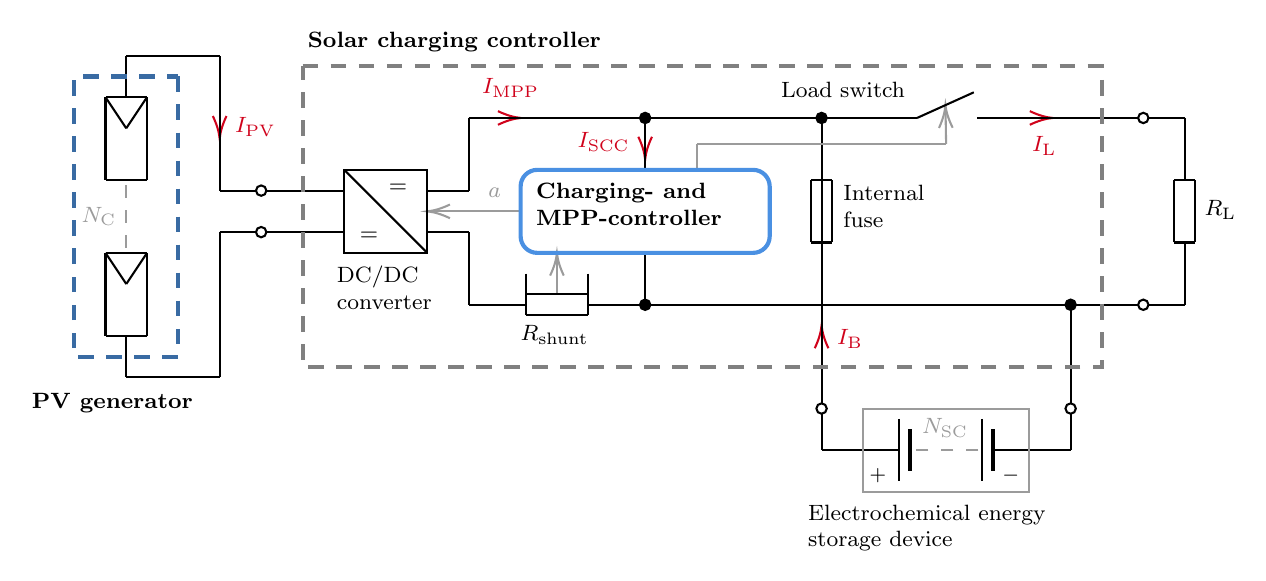
\begin{tikzpicture}[x=0.75pt,y=0.75pt,yscale=-1,xscale=1]
%uncomment if require: \path (0,699); %set diagram left start at 0, and has height of 699

%Straight Lines [id:da9421417995427921] 
\draw [color={rgb, 255:red, 208; green, 2; blue, 27 }  ,draw opacity=1 ]   (340,135) -- (340,148) ;
\draw [shift={(340,150)}, rotate = 270] [color={rgb, 255:red, 208; green, 2; blue, 27 }  ,draw opacity=1 ][line width=0.75]    (10.93,-3.29) .. controls (6.95,-1.4) and (3.31,-0.3) .. (0,0) .. controls (3.31,0.3) and (6.95,1.4) .. (10.93,3.29)   ;
%Straight Lines [id:da11882011111847857] 
\draw [color={rgb, 255:red, 208; green, 2; blue, 27 }  ,draw opacity=1 ]   (265,130) -- (278,130) ;
\draw [shift={(280,130)}, rotate = 180] [color={rgb, 255:red, 208; green, 2; blue, 27 }  ,draw opacity=1 ][line width=0.75]    (10.93,-3.29) .. controls (6.95,-1.4) and (3.31,-0.3) .. (0,0) .. controls (3.31,0.3) and (6.95,1.4) .. (10.93,3.29)   ;
%Straight Lines [id:da5374030929898519] 
\draw [color={rgb, 255:red, 155; green, 155; blue, 155 }  ,draw opacity=1 ]   (297.5,215) -- (297.5,197) ;
\draw [shift={(297.5,195)}, rotate = 450] [color={rgb, 255:red, 155; green, 155; blue, 155 }  ,draw opacity=1 ][line width=0.75]    (10.93,-3.29) .. controls (6.95,-1.4) and (3.31,-0.3) .. (0,0) .. controls (3.31,0.3) and (6.95,1.4) .. (10.93,3.29)   ;
%Straight Lines [id:da1989790363552124] 
\draw [color={rgb, 255:red, 208; green, 2; blue, 27 }  ,draw opacity=1 ]   (521.25,130) -- (534.25,130) ;
\draw [shift={(536.25,130)}, rotate = 180] [color={rgb, 255:red, 208; green, 2; blue, 27 }  ,draw opacity=1 ][line width=0.75]    (10.93,-3.29) .. controls (6.95,-1.4) and (3.31,-0.3) .. (0,0) .. controls (3.31,0.3) and (6.95,1.4) .. (10.93,3.29)   ;
%Straight Lines [id:da21829966681616142] 
\draw [color={rgb, 255:red, 208; green, 2; blue, 27 }  ,draw opacity=1 ]   (425,245) -- (425,232) ;
\draw [shift={(425,230)}, rotate = 450] [color={rgb, 255:red, 208; green, 2; blue, 27 }  ,draw opacity=1 ][line width=0.75]    (10.93,-3.29) .. controls (6.95,-1.4) and (3.31,-0.3) .. (0,0) .. controls (3.31,0.3) and (6.95,1.4) .. (10.93,3.29)   ;
%Straight Lines [id:da03029227215015773] 
\draw [color={rgb, 255:red, 208; green, 2; blue, 27 }  ,draw opacity=1 ]   (135,120) -- (135,138) ;
\draw [shift={(135,140)}, rotate = 270] [color={rgb, 255:red, 208; green, 2; blue, 27 }  ,draw opacity=1 ][line width=0.75]    (10.93,-3.29) .. controls (6.95,-1.4) and (3.31,-0.3) .. (0,0) .. controls (3.31,0.3) and (6.95,1.4) .. (10.93,3.29)   ;
%Straight Lines [id:da02274138666088943] 
\draw    (135,165) -- (135,100) ;
%Straight Lines [id:da9018683092685658] 
\draw [color={rgb, 255:red, 155; green, 155; blue, 155 }  ,draw opacity=1 ]   (365,155) -- (365,142.5) ;
%Straight Lines [id:da3536205977605156] 
\draw [color={rgb, 255:red, 155; green, 155; blue, 155 }  ,draw opacity=1 ]   (484.71,125.83) -- (485,142.5) ;
\draw [shift={(484.67,123.83)}, rotate = 88.99] [color={rgb, 255:red, 155; green, 155; blue, 155 }  ,draw opacity=1 ][line width=0.75]    (10.93,-3.29) .. controls (6.95,-1.4) and (3.31,-0.3) .. (0,0) .. controls (3.31,0.3) and (6.95,1.4) .. (10.93,3.29)   ;
%Straight Lines [id:da3940961623559218] 
\draw [color={rgb, 255:red, 155; green, 155; blue, 155 }  ,draw opacity=1 ] [dash pattern={on 4.5pt off 4.5pt}]  (90,192.5) -- (90,157.5) ;
%Straight Lines [id:da305486791416246] 
\draw    (100,120) -- (80,120) ;
%Straight Lines [id:da18383705888296387] 
\draw    (100,120) -- (90,135) ;
%Straight Lines [id:da3095194315665788] 
\draw    (90,135) -- (80,120) ;
%Straight Lines [id:da698747256222205] 
\draw    (100,120) -- (100,160) ;
%Straight Lines [id:da9106612303236621] 
\draw    (80,120) -- (80,160) ;
%Straight Lines [id:da2775343790641671] 
\draw    (100,160) -- (80,160) ;
%Straight Lines [id:da6238057844394507] 
\draw    (90,235) -- (90,255) ;
%Straight Lines [id:da9446915580972504] 
\draw    (90,100) -- (90,120) ;
%Straight Lines [id:da2886170332859268] 
\draw    (100,195) -- (80,195) ;
%Straight Lines [id:da4973666404379713] 
\draw    (100,195) -- (90,210) ;
%Straight Lines [id:da3822755028621725] 
\draw    (90,210) -- (80,195) ;
%Straight Lines [id:da8935801956358882] 
\draw    (100,195) -- (100,235) ;
%Straight Lines [id:da6312155893729114] 
\draw    (80,195) -- (80,235) ;
%Straight Lines [id:da6010711027940552] 
\draw    (100,235) -- (80,235) ;
%Shape: Rectangle [id:dp6783742410505116] 
\draw  [color={rgb, 255:red, 57; green, 107; blue, 163 }  ,draw opacity=1 ][dash pattern={on 5.63pt off 4.5pt}][line width=1.5]  (115,110) -- (115,245) -- (65,245) -- (65,110) -- cycle ;
%Straight Lines [id:da2862092994413896] 
\draw    (90,100) -- (135,100) ;
%Straight Lines [id:da4924615198515234] 
\draw    (90,255) -- (135,255) ;
%Straight Lines [id:da8029714671125825] 
\draw    (135,185) -- (135,255) ;
%Straight Lines [id:da7764512241735024] 
\draw    (135,165) -- (152.5,165) ;
%Straight Lines [id:da5197356742187318] 
\draw    (135,185) -- (152.5,185) ;
%Shape: Circle [id:dp45159015891408627] 
\draw   (152.5,185) .. controls (152.5,183.62) and (153.62,182.5) .. (155,182.5) .. controls (156.38,182.5) and (157.5,183.62) .. (157.5,185) .. controls (157.5,186.38) and (156.38,187.5) .. (155,187.5) .. controls (153.62,187.5) and (152.5,186.38) .. (152.5,185) -- cycle ;
%Shape: Circle [id:dp8259240874509837] 
\draw   (152.5,165) .. controls (152.5,163.62) and (153.62,162.5) .. (155,162.5) .. controls (156.38,162.5) and (157.5,163.62) .. (157.5,165) .. controls (157.5,166.38) and (156.38,167.5) .. (155,167.5) .. controls (153.62,167.5) and (152.5,166.38) .. (152.5,165) -- cycle ;
%Straight Lines [id:da6710153722448606] 
\draw    (157.5,165) -- (195,165) ;
%Straight Lines [id:da2438484327573136] 
\draw    (157.5,185) -- (195,185) ;
%Straight Lines [id:da014835098389228696] 
\draw    (195,155) -- (235,195) ;
%Straight Lines [id:da591897012695844] 
\draw    (235,185) -- (255,185) ;
%Straight Lines [id:da08002520414789704] 
\draw    (235,165) -- (255,165) ;
%Straight Lines [id:da573801302408715] 
\draw    (255,165) -- (255,130) ;
%Straight Lines [id:da8156706903846436] 
\draw    (255,220) -- (255,185) ;
%Straight Lines [id:da06349281099489246] 
\draw    (255,130) -- (340,130) ;
%Straight Lines [id:da2570308374665804] 
\draw [color={rgb, 255:red, 155; green, 155; blue, 155 }  ,draw opacity=1 ]   (237,175) -- (280,175) ;
\draw [shift={(235,175)}, rotate = 0] [color={rgb, 255:red, 155; green, 155; blue, 155 }  ,draw opacity=1 ][line width=0.75]    (10.93,-3.29) .. controls (6.95,-1.4) and (3.31,-0.3) .. (0,0) .. controls (3.31,0.3) and (6.95,1.4) .. (10.93,3.29)   ;
%Straight Lines [id:da8534254271800685] 
\draw    (340,220) -- (577.5,220) ;
%Straight Lines [id:da6771997897740949] 
\draw    (340,130) -- (340,155) ;
%Straight Lines [id:da4018491949490153] 
\draw    (340,220) -- (340,195) ;
%Shape: Square [id:dp006137277495093407] 
\draw   (195,155) -- (235,155) -- (235,195) -- (195,195) -- cycle ;
%Shape: Circle [id:dp7845577348540074] 
\draw  [fill={rgb, 255:red, 0; green, 0; blue, 0 }  ,fill opacity=1 ] (340,217.5) .. controls (341.38,217.5) and (342.5,218.62) .. (342.5,220) .. controls (342.5,221.38) and (341.38,222.5) .. (340,222.5) .. controls (338.62,222.5) and (337.5,221.38) .. (337.5,220) .. controls (337.5,218.62) and (338.62,217.5) .. (340,217.5) -- cycle ;
%Shape: Circle [id:dp8572849216277822] 
\draw  [fill={rgb, 255:red, 0; green, 0; blue, 0 }  ,fill opacity=1 ] (340,127.5) .. controls (341.38,127.5) and (342.5,128.62) .. (342.5,130) .. controls (342.5,131.38) and (341.38,132.5) .. (340,132.5) .. controls (338.62,132.5) and (337.5,131.38) .. (337.5,130) .. controls (337.5,128.62) and (338.62,127.5) .. (340,127.5) -- cycle ;
%Straight Lines [id:da3780211255481636] 
\draw    (524.5,290) -- (545,290) ;
%Straight Lines [id:da03184575218832286] 
\draw    (425,290) -- (445,290) ;
%Straight Lines [id:da2327687009499042] 
\draw [line width=0.75]    (462.5,275) -- (462.5,305) ;
%Straight Lines [id:da6973962605147832] 
\draw [color={rgb, 255:red, 155; green, 155; blue, 155 }  ,draw opacity=1 ] [dash pattern={on 4.5pt off 4.5pt}]  (500.5,290) -- (465.5,290) ;
%Straight Lines [id:da942581709626162] 
\draw [line width=1.5]    (467.5,280) -- (467.5,300) ;
%Straight Lines [id:da9460540646491606] 
\draw [line width=0.75]    (502.5,275) -- (502.5,305) ;
%Straight Lines [id:da815017798843781] 
\draw [line width=1.5]    (507.5,280) -- (507.5,300) ;
%Straight Lines [id:da591654385387534] 
\draw    (462.5,290) -- (445.5,290) ;
%Straight Lines [id:da9349050114513227] 
\draw    (524.5,290) -- (507.5,290) ;
%Shape: Rectangle [id:dp05962945052172275] 
\draw  [color={rgb, 255:red, 155; green, 155; blue, 155 }  ,draw opacity=1 ] (525,270) -- (525,310) -- (445,310) -- (445,270) -- cycle ;
%Shape: Circle [id:dp15752231467223798] 
\draw  [fill={rgb, 255:red, 0; green, 0; blue, 0 }  ,fill opacity=1 ] (425,127.5) .. controls (426.38,127.5) and (427.5,128.62) .. (427.5,130) .. controls (427.5,131.38) and (426.38,132.5) .. (425,132.5) .. controls (423.62,132.5) and (422.5,131.38) .. (422.5,130) .. controls (422.5,128.62) and (423.62,127.5) .. (425,127.5) -- cycle ;
%Shape: Circle [id:dp5007554014602349] 
\draw   (422.5,270) .. controls (422.5,268.62) and (423.62,267.5) .. (425,267.5) .. controls (426.38,267.5) and (427.5,268.62) .. (427.5,270) .. controls (427.5,271.38) and (426.38,272.5) .. (425,272.5) .. controls (423.62,272.5) and (422.5,271.38) .. (422.5,270) -- cycle ;
%Straight Lines [id:da9208992192503083] 
\draw    (545,272.5) -- (545,290) ;
%Straight Lines [id:da627604798253242] 
\draw    (425,272.5) -- (425,290) ;
%Shape: Circle [id:dp2556214449799865] 
\draw   (542.5,270) .. controls (542.5,268.62) and (543.62,267.5) .. (545,267.5) .. controls (546.38,267.5) and (547.5,268.62) .. (547.5,270) .. controls (547.5,271.38) and (546.38,272.5) .. (545,272.5) .. controls (543.62,272.5) and (542.5,271.38) .. (542.5,270) -- cycle ;
%Straight Lines [id:da6463205767083462] 
\draw    (545,220) -- (545,267.5) ;
%Shape: Circle [id:dp5678761425198426] 
\draw  [fill={rgb, 255:red, 0; green, 0; blue, 0 }  ,fill opacity=1 ] (545,217.5) .. controls (546.38,217.5) and (547.5,218.62) .. (547.5,220) .. controls (547.5,221.38) and (546.38,222.5) .. (545,222.5) .. controls (543.62,222.5) and (542.5,221.38) .. (542.5,220) .. controls (542.5,218.62) and (543.62,217.5) .. (545,217.5) -- cycle ;
%Straight Lines [id:da6220082414399177] 
\draw    (425,130) -- (425,267.5) ;
%Straight Lines [id:da2232912850869122] 
\draw    (430,160) -- (420,160) ;
%Straight Lines [id:da5727217442177441] 
\draw    (430,190) -- (420,190) ;
%Straight Lines [id:da19246645036279175] 
\draw    (430,190) -- (430,160) ;
%Straight Lines [id:da4957674579678937] 
\draw    (420,190) -- (420,160) ;
%Shape: Circle [id:dp7355797988494659] 
\draw   (577.5,220) .. controls (577.5,218.62) and (578.62,217.5) .. (580,217.5) .. controls (581.38,217.5) and (582.5,218.62) .. (582.5,220) .. controls (582.5,221.38) and (581.38,222.5) .. (580,222.5) .. controls (578.62,222.5) and (577.5,221.38) .. (577.5,220) -- cycle ;
%Shape: Circle [id:dp40339619027918716] 
\draw   (577.5,130) .. controls (577.5,128.62) and (578.62,127.5) .. (580,127.5) .. controls (581.38,127.5) and (582.5,128.62) .. (582.5,130) .. controls (582.5,131.38) and (581.38,132.5) .. (580,132.5) .. controls (578.62,132.5) and (577.5,131.38) .. (577.5,130) -- cycle ;
%Straight Lines [id:da634111336257325] 
\draw    (577.5,130) -- (500,130) ;
%Straight Lines [id:da13864177091392604] 
\draw    (498.34,117.65) -- (471,130) ;
%Straight Lines [id:da5827331843556056] 
\draw    (471,130) -- (425,130) ;
%Straight Lines [id:da7062937681829833] 
\draw [color={rgb, 255:red, 155; green, 155; blue, 155 }  ,draw opacity=1 ]   (485,142.5) -- (365,142.5) ;
%Rounded Rect [id:dp5103064937946986] 
\draw  [color={rgb, 255:red, 74; green, 144; blue, 226 }  ,draw opacity=1 ][line width=1.5]  (280,163) .. controls (280,158.58) and (283.58,155) .. (288,155) -- (392,155) .. controls (396.42,155) and (400,158.58) .. (400,163) -- (400,187) .. controls (400,191.42) and (396.42,195) .. (392,195) -- (288,195) .. controls (283.58,195) and (280,191.42) .. (280,187) -- cycle ;
%Shape: Rectangle [id:dp17230778221444543] 
\draw  [color={rgb, 255:red, 128; green, 128; blue, 128 }  ,draw opacity=1 ][dash pattern={on 5.63pt off 4.5pt}][line width=1.5]  (175,105) -- (560,105) -- (560,250) -- (175,250) -- cycle ;
%Straight Lines [id:da888966614057181] 
\draw    (605,160) -- (595,160) ;
%Straight Lines [id:da4674825884766862] 
\draw    (605,190) -- (595,190) ;
%Straight Lines [id:da17325028423110056] 
\draw    (595,190) -- (595,160) ;
%Straight Lines [id:da3187482405619504] 
\draw    (605,190) -- (605,160) ;
%Straight Lines [id:da7972051733354486] 
\draw    (582.5,130) -- (600,130) ;
%Straight Lines [id:da18847306710691814] 
\draw    (600,190) -- (600,220) ;
%Straight Lines [id:da5858572022127997] 
\draw    (600,130) -- (600,160) ;
%Straight Lines [id:da09365392979639964] 
\draw    (582.5,220) -- (600,220) ;
%Straight Lines [id:da17780600814069225] 
\draw    (312.5,225) -- (312.5,215) ;
%Straight Lines [id:da9675828109503861] 
\draw    (282.5,225) -- (282.5,215) ;
%Straight Lines [id:da8123532634949631] 
\draw    (282.5,225) -- (312.5,225) ;
%Straight Lines [id:da8259034059803427] 
\draw    (282.5,215) -- (312.5,215) ;
%Straight Lines [id:da44215658235611977] 
\draw    (255,220) -- (282,220) ;
%Straight Lines [id:da6994883602565676] 
\draw    (313,220) -- (340,220) ;
%Straight Lines [id:da5905851393973105] 
\draw    (340,130) -- (425,130) ;
%Straight Lines [id:da49034677151619577] 
\draw    (282.5,205) -- (282.5,215) ;
%Straight Lines [id:da9931250995037515] 
\draw    (312.5,205) -- (312.5,215) ;

% Text Node
\draw (43,261) node [anchor=north west][inner sep=0.75pt]  [font=\footnotesize] [align=left] {\textbf{PV generator}};
% Text Node
\draw (67,171.4) node [anchor=north west][inner sep=0.75pt]  [font=\footnotesize,color={rgb, 255:red, 155; green, 155; blue, 155 }  ,opacity=1 ]  {$N_{\mathrm{C}}$};
% Text Node
\draw (215,160.4) node [anchor=north west][inner sep=0.75pt]  [font=\footnotesize]  {$=$};
% Text Node
\draw (201,183.4) node [anchor=north west][inner sep=0.75pt]  [font=\footnotesize]  {$=$};
% Text Node
\draw (286,160) node [anchor=north west][inner sep=0.75pt]  [font=\footnotesize] [align=left] {\textbf{Charging- and }\\\textbf{MPP-controller}};
% Text Node
\draw (263,162.4) node [anchor=north west][inner sep=0.75pt]  [font=\footnotesize,color={rgb, 255:red, 155; green, 155; blue, 155 }  ,opacity=1 ]  {$a$};
% Text Node
\draw (510.5,297.4) node [anchor=north west][inner sep=0.75pt]  [font=\scriptsize]  {$-$};
% Text Node
\draw (446.5,297.4) node [anchor=north west][inner sep=0.75pt]  [font=\scriptsize]  {$+$};
% Text Node
\draw (472,273.4) node [anchor=north west][inner sep=0.75pt]  [font=\footnotesize,color={rgb, 255:red, 155; green, 155; blue, 155 }  ,opacity=1 ]  {$N_{\mathrm{SC}}$};
% Text Node
\draw (176,87) node [anchor=north west][inner sep=0.75pt]  [font=\footnotesize] [align=left] {\textbf{Solar charging controller}};
% Text Node
\draw (404,111) node [anchor=north west][inner sep=0.75pt]  [font=\footnotesize] [align=left] {Load switch};
% Text Node
\draw (434,161) node [anchor=north west][inner sep=0.75pt]  [font=\footnotesize] [align=left] {Internal\\fuse};
% Text Node
\draw (141,128.4) node [anchor=north west][inner sep=0.75pt]  [font=\footnotesize,color={rgb, 255:red, 208; green, 2; blue, 27 }  ,opacity=1 ]  {$I_{\mathrm{PV}}$};
% Text Node
\draw (431,230.4) node [anchor=north west][inner sep=0.75pt]  [font=\footnotesize,color={rgb, 255:red, 208; green, 2; blue, 27 }  ,opacity=1 ]  {$I_{\mathrm{B}}$};
% Text Node
\draw (417,315) node [anchor=north west][inner sep=0.75pt]  [font=\footnotesize] [align=left] {Electrochemical energy\\storage device};
% Text Node
\draw (525,137.4) node [anchor=north west][inner sep=0.75pt]  [font=\footnotesize,color={rgb, 255:red, 208; green, 2; blue, 27 }  ,opacity=1 ]  {$I_{\mathrm{L}}$};
% Text Node
\draw (608,168.4) node [anchor=north west][inner sep=0.75pt]  [font=\footnotesize]  {$R_{\mathrm{L}}$};
% Text Node
\draw (278.5,228.4) node [anchor=north west][inner sep=0.75pt]  [font=\footnotesize]  {$R_{\mathrm{shunt}}$};
% Text Node
\draw (306,135.4) node [anchor=north west][inner sep=0.75pt]  [font=\footnotesize,color={rgb, 255:red, 208; green, 2; blue, 27 }  ,opacity=1 ]  {$I_{\mathrm{SCC}}$};
% Text Node
\draw (260,109.4) node [anchor=north west][inner sep=0.75pt]  [font=\footnotesize,color={rgb, 255:red, 208; green, 2; blue, 27 }  ,opacity=1 ]  {${I_{\mathrm{MPP}}}$};
% Text Node
\draw (190,200) node [anchor=north west][inner sep=0.75pt]  [font=\footnotesize] [align=left] {DC/DC\\converter};


\end{tikzpicture}

	\caption{The basic structure of a maximum power point tracking solar charging controller. (Recreated from: \cite{Mertens:2015})}
	\label{fig:tikz_SCC}
\end{figure}




\subsection{Electrochemical energy storage} \label{sec:electrochemical}
In order to guarantee a constant supply of electrical energy during times when the PV generator cannot supply the self-sufficient voice communication system, an electrochemical energy storage device is required. Such storage devices are typically rechargeable batteries -- consisting of secondary cells -- based on either lithium, sodium, nickel or lead \cite{Mertens:2015, Sterner:2017, Kurzweil:2018}. 

\emph{Nickel-cadmium} ($\mathrm{NiCd}$) and \emph{nickel-hydrogen} ($\mathrm{NiH}_2$) batteries have long been used for aerospace applications. However, in recent years they have been increasingly replaced by lithium-ion batteries \cite{Ley:2011}. This is due to their high energy density and low self-discharge. On the other hand, the main disadvantages of lithium-ion batteries are high acquisition costs, the need for a \emph{battery management system} (BMS) to maintain safe operation and the strong dependency of the battery performance on the ambient temperatur $\vartheta_{\mathrm{A}}$. The latter becomes a problem only at extreme ambient temperatures \cite{Hausmann:2013, Wehbe:2015, Ala-A.-Hussein:2015, Nejad:2016, Chin:2018}.

In terms of safe operation, \emph{lithium iron phosphate} ($\mathrm{LiFePO}_4$) batteries are among the safest lithium-ion batteries available today. They are furthermore non-toxic\footnote{Compared to, for example, \emph{lithium cobalt oxide} ($\mathrm{LiCoO}_2$) batteries.} and have a very constant cell voltage for different charging states (see linear part in figure \ref{fig:tikz_u_oc_vs_soc}). It is noted that for the \emph{state of charge} $\mathrm{SOC} = 1$ the battery is fully charged and for $\mathrm{SOC} = 0$ it is fully discharged  \cite{Mertens:2015, Sterner:2017, Li:2018, Kurzweil:2018, Hinz:2019, Hossain:2019, Offgridtec:2020}. 

Because $\mathrm{LiFePO}_4$ batteries are commercially available and often used with photvoltaic standalone systems, this subsection aims to model the \emph{terminal voltage} $U_\mathrm{B} = U_\mathrm{B}(\mathrm{SOC})$ in $\left( \mathrm{V} \right)$ of such a battery for a given current $I_\mathrm{B} = I_\mathrm{B}(t)$, based on an experimental approach \cite{Mertens:2015, Offgridtec:2020}. For this purpose, $I_\mathrm{B}(t)$ is defined as shown below:
	\begin{equation} \label{eq:battery_current}
		\centering
		I_\mathrm{B}(t) =
  		\begin{cases}
   			I_\mathrm{D}(t)\text{,} & \text{when discharging the battery} \\
    		- I_\mathrm{C}(t)\text{,} & \text{when charging the battery.}
  		\end{cases}
	\end{equation} 
	
Following from the equation (\ref{eq:battery_current}), the $\mathrm{SOC}$ of a battery as a function of the discharge or charge \emph{time} $t$ in $\left(\mathrm{h}\right)$ can be calculated directly from the \emph{Coulomb counting method} in the equation (\ref{eq:soc}). 
	\begin{equation} \label{eq:soc}
		\centering
		\begin{gathered}
		\mathrm{SOC}(t) = \mathrm{SOC}_\mathrm{init} - \dfrac{\eta_\mathrm{C}}{Q_\mathrm{tot}} \int\limits_{0\mathrm{h}}^{t} I_\mathrm{B}(\tau) \,\mathrm{d}\tau \\
		\mathrm{SOC}(t) = \mathrm{SOC}_\mathrm{init} - \dfrac{\eta_\mathrm{C}}{Q_\mathrm{tot}} \displaystyle\sum_{\tau = 0\mathrm{h}}^{t} I_\mathrm{B}(\tau) \, \Delta \tau
		\end{gathered}
	\end{equation} 
$\mathrm{SOC}_\mathrm{init}$ in $\left(1\right)$ is the \emph{initial} SOC of the battery. It can be calculated by the ratio of the \emph{remaining battery charge} $Q_\mathrm{rem}$ in $\left(\mathrm{Ah}\right)$ to the \emph{total available battery charge} $Q_\mathrm{tot}$ in $\left(\mathrm{Ah}\right)$ as written in the equation (\ref{eq:soc_init}). $\eta_\mathrm{C}$ is the \emph{coulombic efficiency} in $\left(1\right)$ for which $\eta_\mathrm{C} = 1$ applies when discharging and $\eta_\mathrm{C} \leq 1$ applies when charging \cite{He:2011, Wehbe:2015, Nejad:2016, Kurzweil:2018, Li:2018}. In the proposed model it is assumed that $\eta_\mathrm{C} = 1$ applies for both cases \cite{Hentunen:2014, Hinz:2019,Gurjer:2019}.
	\begin{equation} \label{eq:soc_init}
	\centering
		\mathrm{SOC}_\mathrm{init} = \dfrac{Q_\mathrm{rem}}{Q_\mathrm{tot}}
	\end{equation}

According to the authors of \cite{Hausmann:2013, Kurzweil:2018, Saldana:2019}, the total available battery charge $Q_\mathrm{tot}$ when discharging depends on the \emph{discharging current} $I_\mathrm{D}$ in $\left(\mathrm{A}\right)$. During charging -- with the \emph{charging current} $I_\mathrm{C}$ in $\left(\mathrm{A}\right)$ -- $Q_\mathrm{tot}$ is equal to the \emph{nominal battery charge} $Q_\mathrm{nom}$ in $\left(\mathrm{Ah}\right)$. This empirical approximation is summarized in the equation (\ref{eq:battery_charge}), in which $k_\mathrm{P} \approx 1,05$ is the \emph{Peukert constant} for lithium-ion batteries and $Q_\mathrm{nom}$ can be taken from the data sheet of a $\mathrm{LiFePO}_4$ battery \cite{Hausmann:2013, Kurzweil:2018}.
	\begin{equation} \label{eq:battery_charge}
	\centering
		Q_\mathrm{tot} \approx
  		\begin{cases}
   			Q_\mathrm{nom} \left(\dfrac{I_\mathrm{nom}}{I_\mathrm{D}}\right)^{k_\mathrm{P} - 1} \text{,} & \text{when discharging the battery} \\
    		Q_\mathrm{nom}\text{,} & \text{when charging the battery}
  		\end{cases}
	\end{equation} 
	
Since $Q_\mathrm{nom}$ depends on the \emph{discharging rate} $\mathrm{C_D}$ in $\left(\mathrm{h}^{-1}\right)$, which is listed in the data sheet as well, the \emph{nominal battery current} $I_\mathrm{nom}$ in $\left(\mathrm{A}\right)$ can be calculated as follows \cite{Thirugnanam:2014, Kurzweil:2018}: 
	\begin{equation} \label{eq:i_nom}
	\centering
		I_\mathrm{nom} = \mathrm{C_D} \, Q_\mathrm{nom} \text{.}
	\end{equation}
	
From the above it can now be concluded that the \emph{battery charge} as a function of the time $Q_\mathrm{B}(t)$ in $\left(\mathrm{Ah}\right)$ must result in:
\begin{equation} \label{eq:q_b}
\centering
	Q_\mathrm{B}(t) = \mathrm{SOC} \, Q_\mathrm{tot} \text{.}
\end{equation}

The simplest EEC model of a $\mathrm{LiFePO}_4$ battery is an ideal voltage source. Altough this model is easy to implement and compute in simulations, it lacks important properties such as the dynamical behavior of the battery's open-circuit voltage $U_0 = U_0(\mathrm{SOC})$ in $\left( \mathrm{V} \right)$, \emph{electrolyte resistance} when discharging $R_{\mathrm{e,D}} = R_{\mathrm{e,D}}(\mathrm{SOC})$ in $\left( \Omega \right)$ and electrolyte resistance when charging $R_{\mathrm{e,C}} = R_{\mathrm{e,C}}(\mathrm{SOC})$ in $\left( \Omega \right)$. To incorporate these properties and improve accuracy while keeping the model simple, the $R_{\mathrm{int}}$ model shown in the figure (\ref{fig:tikz_simple_battery_model}) is used. The diodes in this model are assumed to be ideal and are only present to illustrate which resistor is used depending on the sign of $I_\mathrm{B}$ \cite{He:2011, Wehbe:2015, Hinz:2019, Saldana:2019}. 
\begin{figure}[h!]
	\centering
	

\tikzset{every picture/.style={line width=0.75pt}} %set default line width to 0.75pt        

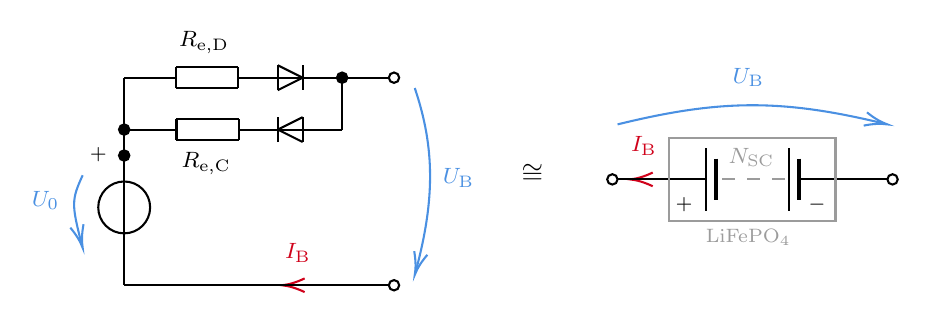
\begin{tikzpicture}[x=0.75pt,y=0.75pt,yscale=-1,xscale=1]
%uncomment if require: \path (0,538); %set diagram left start at 0, and has height of 538

%Straight Lines [id:da4239899953329598] 
\draw [color={rgb, 255:red, 208; green, 2; blue, 27 }  ,draw opacity=1 ]   (353.7,89) -- (340.7,89) ;
\draw [shift={(338.7,89)}, rotate = 360] [color={rgb, 255:red, 208; green, 2; blue, 27 }  ,draw opacity=1 ][line width=0.75]    (10.93,-3.29) .. controls (6.95,-1.4) and (3.31,-0.3) .. (0,0) .. controls (3.31,0.3) and (6.95,1.4) .. (10.93,3.29)   ;
%Straight Lines [id:da9141076711022191] 
\draw    (437.2,89) -- (462.7,89) ;
%Straight Lines [id:da7287140172069071] 
\draw    (332.7,89) -- (358.2,89) ;
%Straight Lines [id:da4302627140031041] 
\draw [line width=0.75]    (375.2,74) -- (375.2,104) ;
%Straight Lines [id:da913986115400165] 
\draw [color={rgb, 255:red, 155; green, 155; blue, 155 }  ,draw opacity=1 ] [dash pattern={on 4.5pt off 4.5pt}]  (413.2,89) -- (378.2,89) ;
%Straight Lines [id:da0409458343135809] 
\draw [line width=1.5]    (380.2,79) -- (380.2,99) ;
%Straight Lines [id:da4345075547353312] 
\draw [line width=0.75]    (415.2,74) -- (415.2,104) ;
%Straight Lines [id:da5169457053238025] 
\draw [line width=1.5]    (420.2,79) -- (420.2,99) ;
%Straight Lines [id:da41248947519842916] 
\draw    (375.2,89) -- (358.2,89) ;
%Straight Lines [id:da6713245296000157] 
\draw    (437.2,89) -- (420.2,89) ;
%Shape: Rectangle [id:dp8204842146016547] 
\draw  [color={rgb, 255:red, 155; green, 155; blue, 155 }  ,draw opacity=1 ] (437.7,69) -- (437.7,109) -- (357.7,109) -- (357.7,69) -- cycle ;
%Shape: Circle [id:dp05668955637455353] 
\draw   (462.7,89) .. controls (462.7,87.62) and (463.82,86.5) .. (465.2,86.5) .. controls (466.58,86.5) and (467.7,87.62) .. (467.7,89) .. controls (467.7,90.38) and (466.58,91.5) .. (465.2,91.5) .. controls (463.82,91.5) and (462.7,90.38) .. (462.7,89) -- cycle ;
%Shape: Circle [id:dp33107549337961006] 
\draw   (327.7,89) .. controls (327.7,87.62) and (328.82,86.5) .. (330.2,86.5) .. controls (331.58,86.5) and (332.7,87.62) .. (332.7,89) .. controls (332.7,90.38) and (331.58,91.5) .. (330.2,91.5) .. controls (328.82,91.5) and (327.7,90.38) .. (327.7,89) -- cycle ;
%Straight Lines [id:da2443541757815666] 
\draw    (150.2,70) -- (150.2,60) ;
%Straight Lines [id:da3018326941100804] 
\draw    (120.2,70) -- (120.2,60) ;
%Straight Lines [id:da09587352502061908] 
\draw    (120.2,60) -- (150.2,60) ;
%Straight Lines [id:da3763833295474801] 
\draw    (120.2,70) -- (150.2,70) ;
%Shape: Circle [id:dp1439179539445421] 
\draw   (222.5,140) .. controls (222.5,138.62) and (223.62,137.5) .. (225,137.5) .. controls (226.38,137.5) and (227.5,138.62) .. (227.5,140) .. controls (227.5,141.38) and (226.38,142.5) .. (225,142.5) .. controls (223.62,142.5) and (222.5,141.38) .. (222.5,140) -- cycle ;
%Curve Lines [id:da3331566122014491] 
\draw [color={rgb, 255:red, 74; green, 144; blue, 226 }  ,draw opacity=1 ]   (235,45) .. controls (244.85,74.06) and (244.67,99.07) .. (235.43,133.42) ;
\draw [shift={(235,135)}, rotate = 285.37] [color={rgb, 255:red, 74; green, 144; blue, 226 }  ,draw opacity=1 ][line width=0.75]    (10.93,-3.29) .. controls (6.95,-1.4) and (3.31,-0.3) .. (0,0) .. controls (3.31,0.3) and (6.95,1.4) .. (10.93,3.29)   ;
%Straight Lines [id:da12346349600905393] 
\draw    (120,65) -- (95,65) ;
%Straight Lines [id:da5810641195940982] 
\draw    (200,65) -- (150,65) ;
%Curve Lines [id:da7444420801068847] 
\draw [color={rgb, 255:red, 74; green, 144; blue, 226 }  ,draw opacity=1 ]   (332.7,62.5) .. controls (382.2,50.32) and (412.1,50.2) .. (461.21,62.13) ;
\draw [shift={(462.7,62.5)}, rotate = 193.82] [color={rgb, 255:red, 74; green, 144; blue, 226 }  ,draw opacity=1 ][line width=0.75]    (10.93,-3.29) .. controls (6.95,-1.4) and (3.31,-0.3) .. (0,0) .. controls (3.31,0.3) and (6.95,1.4) .. (10.93,3.29)   ;
%Straight Lines [id:da5618088487512516] 
\draw    (169,65) -- (169,59) ;
%Straight Lines [id:da29118090532809715] 
\draw    (169,71) -- (169,65) ;
%Straight Lines [id:da2431889749598486] 
\draw    (181,65) -- (181,59) ;
%Straight Lines [id:da9775548645016445] 
\draw    (181,71) -- (181,65) ;
%Straight Lines [id:da3216931327964543] 
\draw    (181,59) -- (169,65) ;
%Straight Lines [id:da870976741839419] 
\draw    (169,65) -- (181,71) ;

%Straight Lines [id:da29875361444983284] 
\draw    (181,40) -- (181,46) ;
%Straight Lines [id:da7309428237562423] 
\draw    (181,34) -- (181,40) ;
%Straight Lines [id:da11204992783900991] 
\draw    (169,40) -- (169,46) ;
%Straight Lines [id:da5502664053025084] 
\draw    (169,34) -- (169,40) ;
%Straight Lines [id:da8629778980345648] 
\draw    (169,46) -- (181,40) ;
%Straight Lines [id:da5424096411610386] 
\draw    (181,40) -- (169,34) ;

%Straight Lines [id:da9431912791064043] 
\draw    (150,45) -- (150,35) ;
%Straight Lines [id:da27346319108632255] 
\draw    (120,45) -- (120,35) ;
%Straight Lines [id:da20640200546003817] 
\draw    (120,35) -- (150,35) ;
%Straight Lines [id:da18589465192348942] 
\draw    (120,45) -- (150,45) ;
%Straight Lines [id:da6749045511361336] 
\draw    (120,40) -- (95,40) ;
%Straight Lines [id:da6054813975075914] 
\draw    (200,40) -- (150,40) ;
%Curve Lines [id:da20601837869887363] 
\draw [color={rgb, 255:red, 74; green, 144; blue, 226 }  ,draw opacity=1 ]   (75,87) .. controls (69.66,98.64) and (69.5,100.87) .. (74.52,120.16) ;
\draw [shift={(75,122)}, rotate = 255.32] [color={rgb, 255:red, 74; green, 144; blue, 226 }  ,draw opacity=1 ][line width=0.75]    (10.93,-3.29) .. controls (6.95,-1.4) and (3.31,-0.3) .. (0,0) .. controls (3.31,0.3) and (6.95,1.4) .. (10.93,3.29)   ;
%Straight Lines [id:da9173542167140516] 
\draw    (95,115) -- (95,140) ;
%Shape: Circle [id:dp7890429606576399] 
\draw   (82.5,102.5) .. controls (82.5,95.6) and (88.1,90) .. (95,90) .. controls (101.9,90) and (107.5,95.6) .. (107.5,102.5) .. controls (107.5,109.4) and (101.9,115) .. (95,115) .. controls (88.1,115) and (82.5,109.4) .. (82.5,102.5) -- cycle ;
%Straight Lines [id:da13008642308028828] 
\draw    (95,90) -- (95,115) ;
%Shape: Circle [id:dp15390548847390928] 
\draw  [fill={rgb, 255:red, 0; green, 0; blue, 0 }  ,fill opacity=1 ] (92.5,65) .. controls (92.5,63.62) and (93.62,62.5) .. (95,62.5) .. controls (96.38,62.5) and (97.5,63.62) .. (97.5,65) .. controls (97.5,66.38) and (96.38,67.5) .. (95,67.5) .. controls (93.62,67.5) and (92.5,66.38) .. (92.5,65) -- cycle ;
%Straight Lines [id:da8926418883187299] 
\draw    (95,65) -- (95,90) ;
%Shape: Circle [id:dp8701642887336025] 
\draw  [fill={rgb, 255:red, 0; green, 0; blue, 0 }  ,fill opacity=1 ] (92.5,77.5) .. controls (92.5,76.12) and (93.62,75) .. (95,75) .. controls (96.38,75) and (97.5,76.12) .. (97.5,77.5) .. controls (97.5,78.88) and (96.38,80) .. (95,80) .. controls (93.62,80) and (92.5,78.88) .. (92.5,77.5) -- cycle ;
%Straight Lines [id:da3048740601702784] 
\draw    (95,40) -- (95,65) ;
%Straight Lines [id:da09511807464774336] 
\draw    (200,40) -- (200,65) ;
%Shape: Circle [id:dp38532315841057274] 
\draw  [fill={rgb, 255:red, 0; green, 0; blue, 0 }  ,fill opacity=1 ] (197.5,40) .. controls (197.5,38.62) and (198.62,37.5) .. (200,37.5) .. controls (201.38,37.5) and (202.5,38.62) .. (202.5,40) .. controls (202.5,41.38) and (201.38,42.5) .. (200,42.5) .. controls (198.62,42.5) and (197.5,41.38) .. (197.5,40) -- cycle ;
%Straight Lines [id:da8764452950084511] 
\draw    (222.5,40) -- (200,40) ;
%Shape: Circle [id:dp3596370907961366] 
\draw   (222.5,40) .. controls (222.5,38.62) and (223.62,37.5) .. (225,37.5) .. controls (226.38,37.5) and (227.5,38.62) .. (227.5,40) .. controls (227.5,41.38) and (226.38,42.5) .. (225,42.5) .. controls (223.62,42.5) and (222.5,41.38) .. (222.5,40) -- cycle ;
%Straight Lines [id:da08595414648708033] 
\draw [color={rgb, 255:red, 208; green, 2; blue, 27 }  ,draw opacity=1 ]   (186,140) -- (173,140) ;
\draw [shift={(171,140)}, rotate = 360] [color={rgb, 255:red, 208; green, 2; blue, 27 }  ,draw opacity=1 ][line width=0.75]    (10.93,-3.29) .. controls (6.95,-1.4) and (3.31,-0.3) .. (0,0) .. controls (3.31,0.3) and (6.95,1.4) .. (10.93,3.29)   ;
%Straight Lines [id:da5785984434842868] 
\draw    (95,140) -- (222.5,140) ;

% Text Node
\draw (373.7,111.4) node [anchor=north west][inner sep=0.75pt]  [font=\scriptsize,color={rgb, 255:red, 0; green, 0; blue, 0 }  ,opacity=1 ]  {$\mathrm{\textcolor[rgb]{0.61,0.61,0.61}{LiFePO}\textcolor[rgb]{0.61,0.61,0.61}{_{4}}}$};
% Text Node
\draw (423.2,96.4) node [anchor=north west][inner sep=0.75pt]  [font=\scriptsize]  {$-$};
% Text Node
\draw (359.2,96.4) node [anchor=north west][inner sep=0.75pt]  [font=\scriptsize]  {$+$};
% Text Node
\draw (384.7,72.4) node [anchor=north west][inner sep=0.75pt]  [font=\footnotesize,color={rgb, 255:red, 155; green, 155; blue, 155 }  ,opacity=1 ]  {$N_{\mathrm{SC}}$};
% Text Node
\draw (285,80.4) node [anchor=north west][inner sep=0.75pt]  [font=\normalsize]  {$\cong $};
% Text Node
\draw (247,82.4) node [anchor=north west][inner sep=0.75pt]  [font=\footnotesize,color={rgb, 255:red, 74; green, 144; blue, 226 }  ,opacity=1 ]  {$U_{\mathrm{B}}$};
% Text Node
\draw (386.7,33.9) node [anchor=north west][inner sep=0.75pt]  [font=\footnotesize,color={rgb, 255:red, 74; green, 144; blue, 226 }  ,opacity=1 ]  {$U_{\mathrm{B}}$};
% Text Node
\draw (337.7,66.9) node [anchor=north west][inner sep=0.75pt]  [font=\footnotesize,color={rgb, 255:red, 208; green, 2; blue, 27 }  ,opacity=1 ]  {$I_{\mathrm{B}}$};
% Text Node
\draw (49,93.4) node [anchor=north west][inner sep=0.75pt]  [font=\footnotesize,color={rgb, 255:red, 74; green, 144; blue, 226 }  ,opacity=1 ]  {$U_{0}$};
% Text Node
\draw (77,71.9) node [anchor=north west][inner sep=0.75pt]  [font=\scriptsize]  {$+$};
% Text Node
\draw (171,118.4) node [anchor=north west][inner sep=0.75pt]  [font=\footnotesize,color={rgb, 255:red, 208; green, 2; blue, 27 }  ,opacity=1 ]  {$I_{\mathrm{B}}$};
% Text Node
\draw (120,16.4) node [anchor=north west][inner sep=0.75pt]  [font=\footnotesize]  {$R_{\mathrm{e,D}}$};
% Text Node
\draw (121.2,74.4) node [anchor=north west][inner sep=0.75pt]  [font=\footnotesize]  {$R_{\mathrm{e,C}}$};


\end{tikzpicture}

	\caption{$R_{\mathrm{int}}$ model of a $\mathrm{LiFePO}_4$ battery (electrochemical energy storage device). (Recreated from: \cite{Hinz:2019, Saldana:2019})}
	\label{fig:tikz_simple_battery_model}
\end{figure}

Figure \ref{fig:tikz_u_oc_vs_soc} shows the typical behavior of the open-circuit voltage $U_0$ of a $\mathrm{LiFePO}_4$ battery as a function of the $\mathrm{SOC}$. For the electrolyte resistances $R_{\mathrm{e,D}}(\mathrm{SOC})$ and $R_{\mathrm{e,C}}(\mathrm{SOC})$, however, it is more difficult to create a generalized function curve. This is due to their varying behavior for different $\mathrm{LiFePO}_4$ batteries \cite{Mertens:2015, Sterner:2017, Li:2018, Hinz:2019, Hossain:2019}. 
\begin{figure}[h!]
	\centering
	

\tikzset{every picture/.style={line width=0.75pt}} %set default line width to 0.75pt        

\begin{tikzpicture}[x=0.75pt,y=0.75pt,yscale=-1,xscale=1]
%uncomment if require: \path (0,300); %set diagram left start at 0, and has height of 300

%Image [id:dp25156695856969735] 
\draw (311.78,133.5) node  {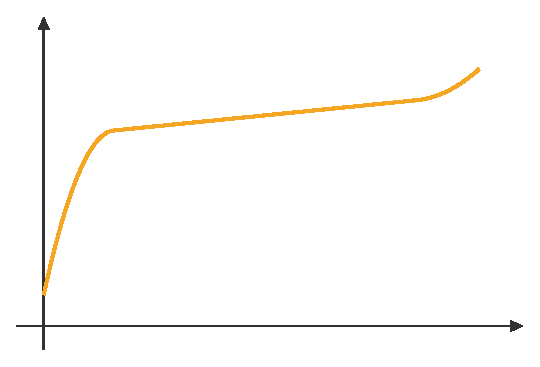
\includegraphics[width=243pt,height=159.75pt]{images/image_u_oc_vs_soc}};
%Straight Lines [id:da24738599691787533] 
\draw [color={rgb, 255:red, 155; green, 155; blue, 155 }  ,draw opacity=1 ] [dash pattern={on 4.5pt off 4.5pt}]  (446.5,59.6) -- (446.23,226.14) ;
%Straight Lines [id:da006125162687165009] 
\draw    (217.33,65) -- (403.33,65) ;
\draw [shift={(405.33,65)}, rotate = 180] [color={rgb, 255:red, 0; green, 0; blue, 0 }  ][line width=0.75]    (10.93,-3.29) .. controls (6.95,-1.4) and (3.31,-0.3) .. (0,0) .. controls (3.31,0.3) and (6.95,1.4) .. (10.93,3.29)   ;
\draw [shift={(215.33,65)}, rotate = 0] [color={rgb, 255:red, 0; green, 0; blue, 0 }  ][line width=0.75]    (10.93,-3.29) .. controls (6.95,-1.4) and (3.31,-0.3) .. (0,0) .. controls (3.31,0.3) and (6.95,1.4) .. (10.93,3.29)   ;
%Straight Lines [id:da953558041904232] 
\draw    (215.33,60) -- (215.33,70) ;
%Straight Lines [id:da48944491555667446] 
\draw    (405.33,60) -- (405.33,70) ;

%Shape: Circle [id:dp3335837862454767] 
\draw  [fill={rgb, 255:red, 255; green, 255; blue, 255 }  ,fill opacity=1 ] (444.5,59.6) .. controls (444.5,58.5) and (445.4,57.6) .. (446.5,57.6) .. controls (447.6,57.6) and (448.5,58.5) .. (448.5,59.6) .. controls (448.5,60.7) and (447.6,61.6) .. (446.5,61.6) .. controls (445.4,61.6) and (444.5,60.7) .. (444.5,59.6) -- cycle ;
%Shape: Circle [id:dp5046748837393529] 
\draw  [fill={rgb, 255:red, 255; green, 255; blue, 255 }  ,fill opacity=1 ] (165.3,202.93) .. controls (165.3,201.83) and (166.2,200.93) .. (167.3,200.93) .. controls (168.4,200.93) and (169.3,201.83) .. (169.3,202.93) .. controls (169.3,204.04) and (168.4,204.93) .. (167.3,204.93) .. controls (166.2,204.93) and (165.3,204.04) .. (165.3,202.93) -- cycle ;
%Shape: Circle [id:dp5166078562699203] 
\draw  [fill={rgb, 255:red, 255; green, 255; blue, 255 }  ,fill opacity=1 ] (175.5,162.27) .. controls (175.5,161.16) and (176.4,160.27) .. (177.5,160.27) .. controls (178.6,160.27) and (179.5,161.16) .. (179.5,162.27) .. controls (179.5,163.37) and (178.6,164.27) .. (177.5,164.27) .. controls (176.4,164.27) and (175.5,163.37) .. (175.5,162.27) -- cycle ;

% Text Node
\draw (142.5,5.4) node [anchor=north west][inner sep=0.75pt]  [font=\footnotesize]  {$U_{0}(\mathrm{SOC})$};
% Text Node
\draw (478.5,218.4) node [anchor=north west][inner sep=0.75pt]  [font=\footnotesize]  {$\mathrm{SOC}$};
% Text Node
\draw (153.33,229.07) node [anchor=north west][inner sep=0.75pt]  [font=\footnotesize]  {$0$};
% Text Node
\draw (441.67,228.4) node [anchor=north west][inner sep=0.75pt]  [font=\footnotesize]  {$1$};
% Text Node
\draw (280,47.4) node [anchor=north west][inner sep=0.75pt]  [font=\footnotesize]  {$\approx \text{Linear}$};
% Text Node
\draw (454,53.4) node [anchor=north west][inner sep=0.75pt]  [font=\footnotesize]  {$\mathrm{SOC}_{N_{\mathrm{MP}}}$};
% Text Node
\draw (186,157.4) node [anchor=north west][inner sep=0.75pt]  [font=\footnotesize]  {$\mathrm{SOC}_{2}$};
% Text Node
\draw (176,197.4) node [anchor=north west][inner sep=0.75pt]  [font=\footnotesize]  {$\mathrm{SOC}_{1}$};
% Text Node
\draw (202.6,138.98) node [anchor=north west][inner sep=0.75pt]  [font=\footnotesize,rotate=-292]  {$\dotsc $};


\end{tikzpicture}



	\caption{Typical behavior of the open-circuit voltage $U_0$ of a $\mathrm{LiFePO}_4$ battery depending on the $\mathrm{SOC}$. $\mathrm{SOC_1}$ to $\mathrm{SOC}_{N_\mathrm{MP}}$ represent the measuring points for the discharging and charging experiment. (Recreated from: \cite{Mertens:2015, Sterner:2017, Li:2018, Hinz:2019, Hossain:2019})}
	\label{fig:tikz_u_oc_vs_soc}
\end{figure}

On this basis, the terminal voltage of the battery $U_\mathrm{B}$ as a function of the SOC, and wether it is being discharged or charged, can be obtained after Kirchhoff's second law is applied to the model \cite{He:2011, Wehbe:2015, Hinz:2019, Saldana:2019}:
	\begin{equation} \label{eq:battery_voltage}
	\centering
		U_\mathrm{B}(\mathrm{SOC}) =
  		\begin{cases}
   			U_0 - R_{\mathrm{e,D}} \, I_\mathrm{D}\text{,} & \text{when discharging the battery} \\
    		U_0 + R_{\mathrm{e,C}} \, I_\mathrm{C}\text{,} & \text{when charging the battery.}
  		\end{cases}
	\end{equation} 
	
At this point it must be made clear that a $\mathrm{LiFePO}_4$ battery is completely discharged when the voltage $U_\mathrm{B} = U_\mathrm{cut-off}$ is reached and fully charged when the voltage $U_\mathrm{B} = U_\mathrm{full}$ is reached \cite{Hinz:2019, Offgridtec:2020}.\footnote{The name \emph{cuf-off voltage} comes from the fact that the BMS turns off the battery to avoid an unsafe state.} If the equations (\ref{eq:battery_voltage}) and (\ref{eq:battery_charge}) are compared, it can be seen that $U_\mathrm{cut-off}$ is reached at a later point in time for smaller currents $I_\mathrm{D}$. This shows that the battery can be discharged more deeply, which manifests itself in a larger total available battery charge $Q_\mathrm{B}$ \cite{Hausmann:2013, Kurzweil:2018}. Here, however, the compromise is made that the cut-off voltage in the proposed model varies for different discharging currents. 

Figure \ref{fig:tikz_pc_pd_battery_curve} shows the behavior of the battery voltage $U_{\mathrm B}(t)$ when it is discharged with a constant current $I_{\mathrm D}$ over the \emph{time interval} $\Delta t_{\mathrm{D}} = t_\mathrm{D, off} - t_\mathrm{D, on}$ in $\left(\mathrm{h}\right)$ and then charged with the constant current $I_{\mathrm C}$ over the time interval $\Delta t_{\mathrm{C}} = t_\mathrm{C, off} - t_\mathrm{C, on}$ in $\left(\mathrm{h}\right)$ \cite{Rahmoun:2012, Hentunen:2014, Li:2018, Kurzweil:2018, Gurjer:2019, Saldana:2019, Hossain:2019}.
\begin{figure}[h!]
	\centering
	

\tikzset{every picture/.style={line width=0.75pt}} %set default line width to 0.75pt        

\begin{tikzpicture}[x=0.75pt,y=0.75pt,yscale=-1,xscale=1]
%uncomment if require: \path (0,399); %set diagram left start at 0, and has height of 399

%Image [id:dp9431825859465086] 
\draw (257.75,202.7) node  {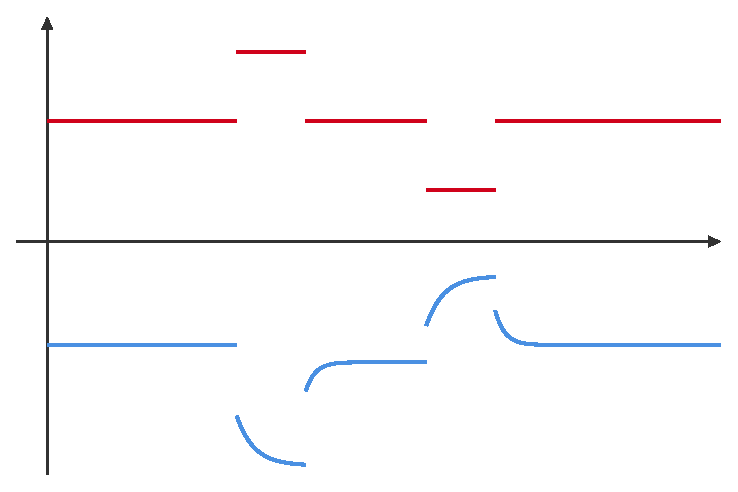
\includegraphics[width=337.88pt,height=219.75pt]{images/image_pc_pd_curve}};
%Straight Lines [id:da7984917488209211] 
\draw [color={rgb, 255:red, 155; green, 155; blue, 155 }  ,draw opacity=1 ] [dash pattern={on 4.5pt off 4.5pt}]  (285,265.7) -- (435,265.7) ;
%Straight Lines [id:da23770186298412455] 
\draw [color={rgb, 255:red, 155; green, 155; blue, 155 }  ,draw opacity=1 ] [dash pattern={on 4.5pt off 4.5pt}]  (59,265.7) -- (250,265.7) ;
%Straight Lines [id:da8950127464122881] 
\draw [color={rgb, 255:red, 74; green, 144; blue, 226 }  ,draw opacity=1 ][line width=1.5]  [dash pattern={on 1.69pt off 2.76pt}]  (173,269.5) -- (173,307.5) ;
%Straight Lines [id:da8271633433271262] 
\draw [color={rgb, 255:red, 74; green, 144; blue, 226 }  ,draw opacity=1 ][line width=1.5]  [dash pattern={on 1.69pt off 2.76pt}]  (217,299.2) -- (217,337.2) ;
%Straight Lines [id:da6802360531812348] 
\draw [color={rgb, 255:red, 74; green, 144; blue, 226 }  ,draw opacity=1 ][line width=1.5]  [dash pattern={on 1.69pt off 2.76pt}]  (294,257) -- (294,272) ;
%Straight Lines [id:da665320735281528] 
\draw [color={rgb, 255:red, 74; green, 144; blue, 226 }  ,draw opacity=1 ][line width=1.5]  [dash pattern={on 1.69pt off 2.76pt}]  (338.5,226) -- (338.5,241) ;
%Straight Lines [id:da5155481731261737] 
\draw [color={rgb, 255:red, 208; green, 2; blue, 27 }  ,draw opacity=1 ][line width=1.5]  [dash pattern={on 1.69pt off 2.76pt}]  (173.5,84.5) -- (173.5,119.5) ;
%Straight Lines [id:da010424395564271549] 
\draw [color={rgb, 255:red, 208; green, 2; blue, 27 }  ,draw opacity=1 ][line width=1.5]  [dash pattern={on 1.69pt off 2.76pt}]  (217.5,85.5) -- (217.5,120.5) ;
%Straight Lines [id:da3234870226616544] 
\draw [color={rgb, 255:red, 208; green, 2; blue, 27 }  ,draw opacity=1 ][line width=1.5]  [dash pattern={on 1.69pt off 2.76pt}]  (295,128.5) -- (295,163.5) ;
%Straight Lines [id:da1669627999747061] 
\draw [color={rgb, 255:red, 208; green, 2; blue, 27 }  ,draw opacity=1 ][line width=1.5]  [dash pattern={on 1.69pt off 2.76pt}]  (338.5,128.5) -- (338.5,163.5) ;
%Straight Lines [id:da7336073832767973] 
\draw [color={rgb, 255:red, 155; green, 155; blue, 155 }  ,draw opacity=1 ] [dash pattern={on 4.5pt off 4.5pt}]  (180.5,122.5) -- (216.5,122.5) ;
%Straight Lines [id:da38951316698254357] 
\draw    (231,339.63) -- (231,299.5) ;
\draw [shift={(231,297.5)}, rotate = 450] [color={rgb, 255:red, 0; green, 0; blue, 0 }  ][line width=0.75]    (10.93,-3.29) .. controls (6.95,-1.4) and (3.31,-0.3) .. (0,0) .. controls (3.31,0.3) and (6.95,1.4) .. (10.93,3.29)   ;
\draw [shift={(231,341.63)}, rotate = 270] [color={rgb, 255:red, 0; green, 0; blue, 0 }  ][line width=0.75]    (10.93,-3.29) .. controls (6.95,-1.4) and (3.31,-0.3) .. (0,0) .. controls (3.31,0.3) and (6.95,1.4) .. (10.93,3.29)   ;
%Straight Lines [id:da35829040806212764] 
\draw    (236,342.16) -- (226,342.16) ;

%Straight Lines [id:da8393771568930704] 
\draw    (226,297) -- (236,297) ;

%Straight Lines [id:da20675405566740057] 
\draw [color={rgb, 255:red, 155; green, 155; blue, 155 }  ,draw opacity=1 ] [dash pattern={on 4.5pt off 4.5pt}]  (58,78.5) -- (169,78.5) ;
%Straight Lines [id:da3893499978016637] 
\draw [color={rgb, 255:red, 155; green, 155; blue, 155 }  ,draw opacity=1 ] [dash pattern={on 4.5pt off 4.5pt}]  (57,166.7) -- (291,166.7) ;
%Straight Lines [id:da14032166669051893] 
\draw [color={rgb, 255:red, 54; green, 162; blue, 138 }  ,draw opacity=1 ]   (52.2,265.7) -- (173,265.7) ;
%Straight Lines [id:da830483625109742] 
\draw [color={rgb, 255:red, 54; green, 162; blue, 138 }  ,draw opacity=1 ]   (173,265.7) -- (173,310.7) ;
%Straight Lines [id:da8193661154783456] 
\draw [color={rgb, 255:red, 54; green, 162; blue, 138 }  ,draw opacity=1 ]   (217,276.7) -- (294,276.7) ;
%Straight Lines [id:da5334736769051522] 
\draw [color={rgb, 255:red, 54; green, 162; blue, 138 }  ,draw opacity=1 ]   (217,276.7) -- (217,321.7) ;
%Straight Lines [id:da910430036604543] 
\draw [color={rgb, 255:red, 54; green, 162; blue, 138 }  ,draw opacity=1 ]   (173,310.7) -- (217,321.7) ;
%Straight Lines [id:da21771101198750498] 
\draw [color={rgb, 255:red, 54; green, 162; blue, 138 }  ,draw opacity=1 ]   (294,253.7) -- (294,276.7) ;
%Straight Lines [id:da8239917812667736] 
\draw [color={rgb, 255:red, 54; green, 162; blue, 138 }  ,draw opacity=1 ]   (311,330) -- (336,330) ;
%Straight Lines [id:da009949911281480484] 
\draw [color={rgb, 255:red, 54; green, 162; blue, 138 }  ,draw opacity=1 ]   (338.5,242.7) -- (338.5,265.7) ;
%Straight Lines [id:da553277774653504] 
\draw [color={rgb, 255:red, 54; green, 162; blue, 138 }  ,draw opacity=1 ]   (338.5,265.7) -- (482.7,265.7) ;
%Straight Lines [id:da4348739238851991] 
\draw [color={rgb, 255:red, 54; green, 162; blue, 138 }  ,draw opacity=1 ]   (294,253.7) -- (338.5,242.7) ;
%Straight Lines [id:da536977341179073] 
\draw [color={rgb, 255:red, 155; green, 155; blue, 155 }  ,draw opacity=1 ] [dash pattern={on 4.5pt off 4.5pt}]  (301,122.5) -- (337,122.5) ;
%Straight Lines [id:da4017649297581949] 
\draw    (280.89,237.56) -- (280.89,252.56) ;
%Straight Lines [id:da6514598025702074] 
\draw    (351.45,204.9) -- (351.45,219.9) ;
%Straight Lines [id:da6789214017371121] 
\draw    (351.45,245.68) -- (351.45,260.68) ;
%Straight Lines [id:da8572632508349955] 
\draw    (280.89,276.33) -- (280.89,254.56) ;
\draw [shift={(280.89,254.56)}, rotate = 270] [color={rgb, 255:red, 0; green, 0; blue, 0 }  ][line width=0.75]    (10.93,-3.29) .. controls (6.95,-1.4) and (3.31,-0.3) .. (0,0) .. controls (3.31,0.3) and (6.95,1.4) .. (10.93,3.29)   ;
\draw [shift={(280.89,276.33)}, rotate = 450] [color={rgb, 255:red, 0; green, 0; blue, 0 }  ][line width=0.75]    (10.93,-3.29) .. controls (6.95,-1.4) and (3.31,-0.3) .. (0,0) .. controls (3.31,0.3) and (6.95,1.4) .. (10.93,3.29)   ;
%Straight Lines [id:da6742965413146893] 
\draw    (285.89,254.27) -- (275.89,254.27) ;
%Straight Lines [id:da3735265920193138] 
\draw    (275.89,276.61) -- (285.89,276.61) ;

%Straight Lines [id:da4089848528137756] 
\draw    (280.89,278.33) -- (280.89,293.33) ;
%Straight Lines [id:da6377765727461617] 
\draw    (351.45,243.68) -- (351.45,221.9) ;
\draw [shift={(351.45,221.9)}, rotate = 270] [color={rgb, 255:red, 0; green, 0; blue, 0 }  ][line width=0.75]    (10.93,-3.29) .. controls (6.95,-1.4) and (3.31,-0.3) .. (0,0) .. controls (3.31,0.3) and (6.95,1.4) .. (10.93,3.29)   ;
\draw [shift={(351.45,243.68)}, rotate = 450] [color={rgb, 255:red, 0; green, 0; blue, 0 }  ][line width=0.75]    (10.93,-3.29) .. controls (6.95,-1.4) and (3.31,-0.3) .. (0,0) .. controls (3.31,0.3) and (6.95,1.4) .. (10.93,3.29)   ;
%Straight Lines [id:da4999891213389307] 
\draw    (356.45,221.62) -- (346.45,221.62) ;
%Straight Lines [id:da21342574530244263] 
\draw    (346.45,243.96) -- (356.45,243.96) ;

%Straight Lines [id:da38332448511266115] 
\draw    (160.11,308.3) -- (160.11,268.17) ;
\draw [shift={(160.11,266.17)}, rotate = 450] [color={rgb, 255:red, 0; green, 0; blue, 0 }  ][line width=0.75]    (10.93,-3.29) .. controls (6.95,-1.4) and (3.31,-0.3) .. (0,0) .. controls (3.31,0.3) and (6.95,1.4) .. (10.93,3.29)   ;
\draw [shift={(160.11,310.3)}, rotate = 270] [color={rgb, 255:red, 0; green, 0; blue, 0 }  ][line width=0.75]    (10.93,-3.29) .. controls (6.95,-1.4) and (3.31,-0.3) .. (0,0) .. controls (3.31,0.3) and (6.95,1.4) .. (10.93,3.29)   ;
%Straight Lines [id:da5321486664645252] 
\draw    (165.11,310.83) -- (155.11,310.83) ;

%Straight Lines [id:da08166456175406989] 
\draw    (155.11,265.67) -- (165.11,265.67) ;

%Straight Lines [id:da5101730964523248] 
\draw    (173,195.5) -- (173,203.5) ;
%Straight Lines [id:da2319819541264927] 
\draw    (217,195.5) -- (217,203.5) ;
%Straight Lines [id:da808601911633186] 
\draw    (295,195.5) -- (295,203.5) ;
%Straight Lines [id:da3828209146801427] 
\draw    (339,195.5) -- (339,203.5) ;
%Straight Lines [id:da8203400723269536] 
\draw [color={rgb, 255:red, 208; green, 2; blue, 27 }  ,draw opacity=1 ]   (17,21.33) -- (42,21.33) ;
%Straight Lines [id:da38547811974611657] 
\draw [color={rgb, 255:red, 74; green, 144; blue, 226 }  ,draw opacity=1 ]   (17,41.33) -- (42,41.33) ;


% Text Node
\draw (488,193.4) node [anchor=north west][inner sep=0.75pt]  [font=\footnotesize]  {$t$};
% Text Node
\draw (32,160.4) node [anchor=north west][inner sep=0.75pt]  [font=\footnotesize]  {$I_{\mathrm{C}}$};
% Text Node
\draw (32,73.4) node [anchor=north west][inner sep=0.75pt]  [font=\footnotesize]  {$I_{\mathrm{D}}$};
% Text Node
\draw (29,120.4) node [anchor=north west][inner sep=0.75pt]  [font=\footnotesize]  {$0\mathrm{A}$};
% Text Node
\draw (56.7,245.4) node [anchor=north west][inner sep=0.75pt]  [font=\footnotesize]  {$U_{0}( t=0\mathrm{s})$};
% Text Node
\draw (32.82,205.54) node [anchor=north west][inner sep=0.75pt]  [font=\footnotesize]  {$0\mathrm{s}$};
% Text Node
\draw (125.89,280.96) node [anchor=north west][inner sep=0.75pt]  [font=\footnotesize]  {$\Delta U_{\mathrm{D}}$};
% Text Node
\draw (235.22,313.18) node [anchor=north west][inner sep=0.75pt]  [font=\footnotesize]  {$\Delta U_{\mathrm{D}}$};
% Text Node
\draw (355.3,226.79) node [anchor=north west][inner sep=0.75pt]  [font=\footnotesize]  {$\Delta U_{\mathrm{C}}$};
% Text Node
\draw (248.11,259.57) node [anchor=north west][inner sep=0.75pt]  [font=\footnotesize]  {$\Delta U_{\mathrm{C}}$};
% Text Node
\draw (340,323.4) node [anchor=north west][inner sep=0.75pt]  [font=\footnotesize]  {$U_{\mathrm{B}}( t)\text{ with the } R_{\mathrm{int}}\text{ model}$};
% Text Node
\draw (159,56) node [anchor=north west][inner sep=0.75pt]  [font=\footnotesize] [align=left] {Discharging};
% Text Node
\draw (287.33,100.5) node [anchor=north west][inner sep=0.75pt]  [font=\footnotesize] [align=left] {Charging};
% Text Node
\draw (162.8,178.8) node [anchor=north west][inner sep=0.75pt]  [font=\footnotesize]  {$t_{\mathrm{D} ,\mathrm{on}}$};
% Text Node
\draw (206.4,178.8) node [anchor=north west][inner sep=0.75pt]  [font=\footnotesize]  {$t_{\mathrm{D} ,\mathrm{off}}$};
% Text Node
\draw (285,178.8) node [anchor=north west][inner sep=0.75pt]  [font=\footnotesize]  {$t_{\mathrm{C} ,\mathrm{on}}$};
% Text Node
\draw (328.8,178.8) node [anchor=north west][inner sep=0.75pt]  [font=\footnotesize]  {$t_{\mathrm{C} ,\mathrm{off}}$};
% Text Node
\draw (45,14.73) node [anchor=north west][inner sep=0.75pt]  [font=\footnotesize]  {$I_{\mathrm{B}}( t)$};
% Text Node
\draw (45,34.73) node [anchor=north west][inner sep=0.75pt]  [font=\footnotesize]  {$U_{\mathrm{B}}( t)$};


\end{tikzpicture}




	\caption{Behavior of the battery voltage $U_{\mathrm B}(t)$ when it is first discharged with $I_{\mathrm D}$ and then charged with $I_{\mathrm C}$. From the resulting voltage drop $\Delta U_{\mathrm D}(t_\mathrm{D, on})$ and voltage rise $\Delta U_{\mathrm C}(t_\mathrm{C, on})$, the $R_{int}$ model's electrolyte resistances $R_{e,\mathrm{D}}$ and $R_{e,\mathrm{C}}$ can be calculated. The turquoise curve represents the behavior of the modeled battery voltage. (Recreated from: \cite{Rahmoun:2012, Hentunen:2014, Li:2018, Kurzweil:2018, Gurjer:2019, Saldana:2019, Hossain:2019})}
	\label{fig:tikz_pc_pd_battery_curve}
\end{figure}
From the \emph{dropping voltages} $\Delta U_{\mathrm D}(t_\mathrm{D, on})$ and $\Delta U_{\mathrm C}(t_\mathrm{C, off})$ or \emph{rising voltages} $\Delta U_{\mathrm D}(t_\mathrm{D, off})$ and $\Delta U_{\mathrm C}(t_\mathrm{C, on})$ in $\left( \mathrm{V} \right)$, the $R_{int}$ model's electrolyte resistances $R_{\mathrm{e,D}}$ and $R_{\mathrm{e,C}}$ can be calculated as shown in the equations (\ref{eq:r_0_d}) and (\ref{eq:r_0_c}) \cite{Rahmoun:2012, Hentunen:2014, Kurzweil:2018, Gurjer:2019}. 
\begin{equation}\label{eq:r_0_d}
	\centering
	R_{\mathrm{e,D}}(t) = \left|\dfrac{\Delta U_{\mathrm D}}{I_{\mathrm D}}\right|
\end{equation}
\begin{equation}\label{eq:r_0_c}
	\centering
	R_{\mathrm{e,C}}(t) = \left|\dfrac{\Delta U_{\mathrm C}}{I_{\mathrm C}}\right|
\end{equation}
For comparison, the thin turquoise curve represents the behavior of the $R_\mathrm{int}$ model for the same discharge and charge currents $I_{\mathrm D}$ and $I_{\mathrm C}$. At times $t_\mathrm{D, on}$, $t_\mathrm{D, off}$, $t_\mathrm{C, on}$ and $t_\mathrm{C, off}$ it has the same dropping and rising voltages $\Delta U_{\mathrm D}$ and $\Delta U_{\mathrm C}$ as $U_{\mathrm B}(t)$ \cite{Saldana:2019}.

Based on the findings in the articles \cite{Hausmann:2013, Ala-A.-Hussein:2015, Nejad:2016, Chin:2018} it is assumed that $U_0$,  $R_{e,\mathrm{D}}$ and $R_{e,\mathrm{C}}$ do not dependent on the ambient temperature $\vartheta_{\mathrm{A}}$ in the range from $5^\circ \mathrm{C}$ to $45^\circ \mathrm{C}$. Therefore, the proposed model does not apply to temperatures below $5^\circ \mathrm{C}$ and above $45^\circ \mathrm{C}$.

In order to complete the $R_{\mathrm{int}}$ model, the missing properties $U_0(\mathrm{SOC})$, $R_{\mathrm{e,D}}(\mathrm{SOC})$ and $R_{\mathrm{e,C}}(\mathrm{SOC})$ must be determined experimentally. For this purpose, two separate experiments must be carried out as explained in the following paragraphs.

\paragraph*{Discharging experiment:} %% PD EXPERIMENT
The experiment is carried out at the ambient temperature $\vartheta_\mathrm{A} = 25^\circ \mathrm{C}$ with an initially fully charged $\mathrm{LiFePO}_4$ battery ($\mathrm{SOC}_{N_\mathrm{MP}} = 1$) and repeated for the desired \emph{number of measuring points} $N_{\mathrm{MP}}$ in $\left( 1 \right)$, as illustrated in the figure \ref{fig:tikz_u_oc_vs_soc}, until the battery is fully discharged ($\mathrm{SOC}_{1} = 0$) \cite{Rahmoun:2012, Hentunen:2014, Gurjer:2019}. 

A simple measurement setup for this experiment can be seen in the figure \ref{fig:tikz_experiment_1}. $U_\mathrm{shunt}$ in $\left(\mathrm{V}\right)$ is the voltage drop across the shunt resistor $R_\mathrm{shunt}$, measured with \emph{channel 2} (Ch2) of the oscilloscope. On the basis of this voltage drop, $I_\mathrm{L}$ is set so that the battery is discharged with the current:
\begin{equation}\label{eq_i_d_real}
	\centering
I_\mathrm{D} = \dfrac{U_\mathrm{shunt}}{R_\mathrm{shunt}} + I_\mathrm{Ch1} + I_\mathrm{Ch2} \text{.}
\end{equation}
The \emph{measuring currents} $I_\mathrm{Ch1}$ and $I_\mathrm{Ch2}$ in $\left(\mathrm{A}\right)$ caused by the internal resistances of the channels of the oscilloscope are small compared to the load current $I_\mathrm{L}$. Depending on the desired accuracy, $I_\mathrm{Ch1}$ and $I_\mathrm{Ch2}$ can either be neglected or determined by measuring the internal resistances of said channels \cite{Schrufer:2014}.  
\begin{figure}[h!]
	\centering
	

\tikzset{every picture/.style={line width=0.75pt}} %set default line width to 0.75pt        

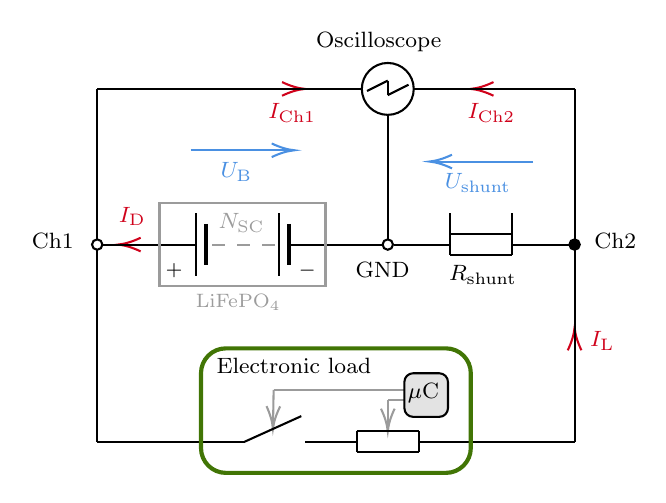
\begin{tikzpicture}[x=0.75pt,y=0.75pt,yscale=-1,xscale=1]
%uncomment if require: \path (0,743); %set diagram left start at 0, and has height of 743

%Straight Lines [id:da045931729156849066] 
\draw [color={rgb, 255:red, 208; green, 2; blue, 27 }  ,draw opacity=1 ]   (285,105) -- (272,105) ;
\draw [shift={(270,105)}, rotate = 360] [color={rgb, 255:red, 208; green, 2; blue, 27 }  ,draw opacity=1 ][line width=0.75]    (10.93,-3.29) .. controls (6.95,-1.4) and (3.31,-0.3) .. (0,0) .. controls (3.31,0.3) and (6.95,1.4) .. (10.93,3.29)   ;
%Straight Lines [id:da3949134308814568] 
\draw    (270,275) -- (320,275) ;
%Straight Lines [id:da08560996153222833] 
\draw [color={rgb, 255:red, 208; green, 2; blue, 27 }  ,draw opacity=1 ]   (115,180) -- (102,180) ;
\draw [shift={(100,180)}, rotate = 360] [color={rgb, 255:red, 208; green, 2; blue, 27 }  ,draw opacity=1 ][line width=0.75]    (10.93,-3.29) .. controls (6.95,-1.4) and (3.31,-0.3) .. (0,0) .. controls (3.31,0.3) and (6.95,1.4) .. (10.93,3.29)   ;
%Straight Lines [id:da050616828595225094] 
\draw    (92.5,180) -- (120.5,180) ;
%Straight Lines [id:da6370801814614784] 
\draw    (200.5,180) -- (227.5,180) ;
%Straight Lines [id:da4527627205165792] 
\draw [color={rgb, 255:red, 208; green, 2; blue, 27 }  ,draw opacity=1 ]   (320,235) -- (320,222) ;
\draw [shift={(320,220)}, rotate = 450] [color={rgb, 255:red, 208; green, 2; blue, 27 }  ,draw opacity=1 ][line width=0.75]    (10.93,-3.29) .. controls (6.95,-1.4) and (3.31,-0.3) .. (0,0) .. controls (3.31,0.3) and (6.95,1.4) .. (10.93,3.29)   ;
%Straight Lines [id:da4189378099752894] 
\draw [color={rgb, 255:red, 208; green, 2; blue, 27 }  ,draw opacity=1 ]   (175,105) -- (188,105) ;
\draw [shift={(190,105)}, rotate = 180] [color={rgb, 255:red, 208; green, 2; blue, 27 }  ,draw opacity=1 ][line width=0.75]    (10.93,-3.29) .. controls (6.95,-1.4) and (3.31,-0.3) .. (0,0) .. controls (3.31,0.3) and (6.95,1.4) .. (10.93,3.29)   ;
%Straight Lines [id:da2658092860751087] 
\draw [line width=0.75]    (137.5,165) -- (137.5,195) ;
%Straight Lines [id:da3949939895399093] 
\draw [color={rgb, 255:red, 155; green, 155; blue, 155 }  ,draw opacity=1 ] [dash pattern={on 4.5pt off 4.5pt}]  (175.5,180) -- (140.5,180) ;
%Straight Lines [id:da6668323928749316] 
\draw [line width=1.5]    (142.5,170) -- (142.5,190) ;
%Straight Lines [id:da2892580654722863] 
\draw [line width=0.75]    (177.5,165) -- (177.5,195) ;
%Straight Lines [id:da305974803365608] 
\draw [line width=1.5]    (182.5,170) -- (182.5,190) ;
%Straight Lines [id:da02397573109880402] 
\draw    (137.5,180) -- (120.5,180) ;
%Straight Lines [id:da31190085768960363] 
\draw    (199.5,180) -- (182.5,180) ;
%Shape: Rectangle [id:dp8008725070360889] 
\draw  [color={rgb, 255:red, 155; green, 155; blue, 155 }  ,draw opacity=1 ] (200,160) -- (200,200) -- (120,200) -- (120,160) -- cycle ;
%Shape: Circle [id:dp20223673484144356] 
\draw   (227.5,180) .. controls (227.5,178.62) and (228.62,177.5) .. (230,177.5) .. controls (231.38,177.5) and (232.5,178.62) .. (232.5,180) .. controls (232.5,181.38) and (231.38,182.5) .. (230,182.5) .. controls (228.62,182.5) and (227.5,181.38) .. (227.5,180) -- cycle ;
%Shape: Circle [id:dp3853206170680481] 
\draw   (87.5,180) .. controls (87.5,178.62) and (88.62,177.5) .. (90,177.5) .. controls (91.38,177.5) and (92.5,178.62) .. (92.5,180) .. controls (92.5,181.38) and (91.38,182.5) .. (90,182.5) .. controls (88.62,182.5) and (87.5,181.38) .. (87.5,180) -- cycle ;
%Straight Lines [id:da5327428480980583] 
\draw    (90,105) -- (90,177.5) ;
%Straight Lines [id:da13935190161788125] 
\draw    (90,105) -- (217.5,105) ;
%Straight Lines [id:da7865577264880768] 
\draw [color={rgb, 255:red, 74; green, 144; blue, 226 }  ,draw opacity=1 ]   (135,134.57) -- (183,134.57) ;
\draw [shift={(185,134.57)}, rotate = 180] [color={rgb, 255:red, 74; green, 144; blue, 226 }  ,draw opacity=1 ][line width=0.75]    (10.93,-3.29) .. controls (6.95,-1.4) and (3.31,-0.3) .. (0,0) .. controls (3.31,0.3) and (6.95,1.4) .. (10.93,3.29)   ;
%Shape: Circle [id:dp3317910125615249] 
\draw   (217.5,105) .. controls (217.5,98.1) and (223.1,92.5) .. (230,92.5) .. controls (236.9,92.5) and (242.5,98.1) .. (242.5,105) .. controls (242.5,111.9) and (236.9,117.5) .. (230,117.5) .. controls (223.1,117.5) and (217.5,111.9) .. (217.5,105) -- cycle ;
%Straight Lines [id:da1875474942123041] 
\draw    (220,106) -- (230,101) ;
%Straight Lines [id:da4090541258718201] 
\draw    (230,101) -- (230,108) ;
%Straight Lines [id:da7457893967384179] 
\draw    (230,108) -- (240,103) ;

%Straight Lines [id:da0917057683123701] 
\draw    (90,182.5) -- (90,275) ;
%Straight Lines [id:da2778004994432466] 
\draw [color={rgb, 255:red, 155; green, 155; blue, 155 }  ,draw opacity=1 ]   (230,255) -- (230,268) ;
\draw [shift={(230,270)}, rotate = 270] [color={rgb, 255:red, 155; green, 155; blue, 155 }  ,draw opacity=1 ][line width=0.75]    (10.93,-3.29) .. controls (6.95,-1.4) and (3.31,-0.3) .. (0,0) .. controls (3.31,0.3) and (6.95,1.4) .. (10.93,3.29)   ;
%Straight Lines [id:da32924484737520543] 
\draw    (245,280) -- (245,270) ;
%Straight Lines [id:da33462944952545204] 
\draw    (215,280) -- (215,270) ;
%Straight Lines [id:da24868968049308626] 
\draw    (215,270) -- (245,270) ;
%Straight Lines [id:da6617574409624216] 
\draw    (215,280) -- (245,280) ;
%Straight Lines [id:da8690193038101492] 
\draw    (215,275) -- (200,275) ;
%Straight Lines [id:da7998432795618544] 
\draw [color={rgb, 255:red, 155; green, 155; blue, 155 }  ,draw opacity=1 ]   (238,255) -- (230,255) ;
%Straight Lines [id:da10758294037064475] 
\draw    (270,275) -- (245,275) ;
%Straight Lines [id:da6790087801319198] 
\draw    (90,275) -- (140,275) ;
%Straight Lines [id:da7635403190384071] 
\draw [color={rgb, 255:red, 155; green, 155; blue, 155 }  ,draw opacity=1 ]   (174.71,266.83) -- (175,250) ;
\draw [shift={(174.67,268.83)}, rotate = 271] [color={rgb, 255:red, 155; green, 155; blue, 155 }  ,draw opacity=1 ][line width=0.75]    (10.93,-3.29) .. controls (6.95,-1.4) and (3.31,-0.3) .. (0,0) .. controls (3.31,0.3) and (6.95,1.4) .. (10.93,3.29)   ;
%Straight Lines [id:da09729743826270276] 
\draw    (205,275) -- (190,275) ;
%Straight Lines [id:da1421569585710698] 
\draw    (188.34,262.65) -- (161,275) ;
%Straight Lines [id:da5452375072503128] 
\draw    (161,275) -- (140,275) ;
%Straight Lines [id:da5345291081584591] 
\draw [color={rgb, 255:red, 155; green, 155; blue, 155 }  ,draw opacity=1 ]   (238,250) -- (175,250) ;
%Rounded Rect [id:dp6576837931168715] 
\draw  [fill={rgb, 255:red, 227; green, 227; blue, 227 }  ,fill opacity=1 ] (238,246.2) .. controls (238,243.88) and (239.88,242) .. (242.2,242) -- (254.8,242) .. controls (257.12,242) and (259,243.88) .. (259,246.2) -- (259,258.8) .. controls (259,261.12) and (257.12,263) .. (254.8,263) -- (242.2,263) .. controls (239.88,263) and (238,261.12) .. (238,258.8) -- cycle ;

%Rounded Rect [id:dp11415612065842651] 
\draw  [color={rgb, 255:red, 65; green, 117; blue, 5 }  ,draw opacity=1 ][line width=1.5]  (140,242) .. controls (140,235.37) and (145.37,230) .. (152,230) -- (258,230) .. controls (264.63,230) and (270,235.37) .. (270,242) -- (270,278) .. controls (270,284.63) and (264.63,290) .. (258,290) -- (152,290) .. controls (145.37,290) and (140,284.63) .. (140,278) -- cycle ;
%Straight Lines [id:da6054782174044755] 
\draw    (320,180) -- (320,275) ;
%Straight Lines [id:da5423361466871042] 
\draw    (242.5,105) -- (320,105) ;
%Straight Lines [id:da9479324460356069] 
\draw    (290,185) -- (290,175) ;
%Straight Lines [id:da8225786744388688] 
\draw    (260,185) -- (260,175) ;
%Straight Lines [id:da05714096809956737] 
\draw    (260,185) -- (290,185) ;
%Straight Lines [id:da8511132029064918] 
\draw    (260,175) -- (290,175) ;
%Straight Lines [id:da6701815168749929] 
\draw    (260,165) -- (260,175) ;
%Straight Lines [id:da41839660929781086] 
\draw    (290,165) -- (290,175) ;
%Shape: Circle [id:dp2800781557119969] 
\draw  [fill={rgb, 255:red, 0; green, 0; blue, 0 }  ,fill opacity=1 ] (320,177.5) .. controls (321.38,177.5) and (322.5,178.62) .. (322.5,180) .. controls (322.5,181.38) and (321.38,182.5) .. (320,182.5) .. controls (318.62,182.5) and (317.5,181.38) .. (317.5,180) .. controls (317.5,178.62) and (318.62,177.5) .. (320,177.5) -- cycle ;
%Straight Lines [id:da2549570467676723] 
\draw    (290,180) -- (320,180) ;
%Straight Lines [id:da2939345663201236] 
\draw    (233,180) -- (260,180) ;
%Straight Lines [id:da832541761407757] 
\draw    (230,117.5) -- (230,177.5) ;
%Straight Lines [id:da19404732115287238] 
\draw [color={rgb, 255:red, 74; green, 144; blue, 226 }  ,draw opacity=1 ]   (300,140) -- (252,140) ;
\draw [shift={(250,140)}, rotate = 360] [color={rgb, 255:red, 74; green, 144; blue, 226 }  ,draw opacity=1 ][line width=0.75]    (10.93,-3.29) .. controls (6.95,-1.4) and (3.31,-0.3) .. (0,0) .. controls (3.31,0.3) and (6.95,1.4) .. (10.93,3.29)   ;

%Straight Lines [id:da8406967180739828] 
\draw    (320,105) -- (320,177.5) ;

% Text Node
\draw (136,202.4) node [anchor=north west][inner sep=0.75pt]  [font=\scriptsize,color={rgb, 255:red, 0; green, 0; blue, 0 }  ,opacity=1 ]  {$\mathrm{\textcolor[rgb]{0.61,0.61,0.61}{LiFePO}\textcolor[rgb]{0.61,0.61,0.61}{_{4}}}$};
% Text Node
\draw (185.5,187.4) node [anchor=north west][inner sep=0.75pt]  [font=\scriptsize]  {$-$};
% Text Node
\draw (121.5,187.4) node [anchor=north west][inner sep=0.75pt]  [font=\scriptsize]  {$+$};
% Text Node
\draw (147,163.4) node [anchor=north west][inner sep=0.75pt]  [font=\footnotesize,color={rgb, 255:red, 155; green, 155; blue, 155 }  ,opacity=1 ]  {$N_{\mathrm{SC}}$};
% Text Node
\draw (148,138.97) node [anchor=north west][inner sep=0.75pt]  [font=\footnotesize,color={rgb, 255:red, 74; green, 144; blue, 226 }  ,opacity=1 ]  {$U_{\mathrm{B}}$};
% Text Node
\draw (99,160.4) node [anchor=north west][inner sep=0.75pt]  [font=\footnotesize,color={rgb, 255:red, 208; green, 2; blue, 27 }  ,opacity=1 ]  {$I_{\mathrm{D}}$};
% Text Node
\draw (171,110.4) node [anchor=north west][inner sep=0.75pt]  [font=\footnotesize,color={rgb, 255:red, 208; green, 2; blue, 27 }  ,opacity=1 ]  {$I_{\mathrm{Ch} 1}$};
% Text Node
\draw (194,76) node [anchor=north west][inner sep=0.75pt]  [font=\footnotesize] [align=left] {Oscilloscope};
% Text Node
\draw (146,233) node [anchor=north west][inner sep=0.75pt]  [font=\footnotesize] [align=left] {Electronic load};
% Text Node
\draw (238.2,245.4) node [anchor=north west][inner sep=0.75pt]  [font=\footnotesize]  {$\mu \mathrm{C}$};
% Text Node
\draw (326,220.4) node [anchor=north west][inner sep=0.75pt]  [font=\footnotesize,color={rgb, 255:red, 208; green, 2; blue, 27 }  ,opacity=1 ]  {$I_{\mathrm{L}}$};
% Text Node
\draw (258,188.4) node [anchor=north west][inner sep=0.75pt]  [font=\footnotesize]  {$R_{\mathrm{shunt}}$};
% Text Node
\draw (267,110.4) node [anchor=north west][inner sep=0.75pt]  [font=\footnotesize,color={rgb, 255:red, 208; green, 2; blue, 27 }  ,opacity=1 ]  {$I_{\mathrm{Ch} 2}$};
% Text Node
\draw (213,187) node [anchor=north west][inner sep=0.75pt]  [font=\footnotesize] [align=left] {GND};
% Text Node
\draw (328,173) node [anchor=north west][inner sep=0.75pt]  [font=\footnotesize] [align=left] {Ch2};
% Text Node
\draw (57,173) node [anchor=north west][inner sep=0.75pt]  [font=\footnotesize] [align=left] {Ch1};
% Text Node
\draw (256,144.4) node [anchor=north west][inner sep=0.75pt]  [font=\footnotesize,color={rgb, 255:red, 74; green, 144; blue, 226 }  ,opacity=1 ]  {$U_{\mathrm{shunt}}$};


\end{tikzpicture}

	\caption{Measurement setup for the discharge experiment.}
	\label{fig:tikz_experiment_1}
\end{figure}

For a certain measuring point $n \in \mathbb{N}$, the battery's open-circuit voltage $U_{0, \mathrm{D}}(\mathrm{SOC}_n)$ in $\left(\mathrm{V}\right)$ is measured with \emph{channel 1} (Ch1) of the oscilloscope. The battery is then discharged using an electronic load in \emph{constant current} (CC) mode\footnote{Even if the battery voltage slowly drops during the course of the experiment, the electronic load will keep the current constant.} with $I_{\mathrm D}$ for $\Delta t_{\mathrm{D}}$ until the desired new measuring point $\mathrm{SOC}_{n-1}$ is reached. At the point in time when the electronic load is switched on, the voltage drop $\Delta U_{\mathrm D}(\mathrm{SOC}_n)$ is measured with Ch1 and the voltage drop $U_\mathrm{shunt}(\mathrm{SOC}_n)$ with Ch2. After the discharge process for $\Delta t_{\mathrm{D}}$ has been completed, the battery must remain idle for the \emph{resting period} $t_\mathrm{rest}$ in $\left( \mathrm{h} \right)$ until the open-circuit voltage has reached an end value (compare to figure \ref{fig:tikz_pc_pd_battery_curve}). When it is reached, the measurements can be repeated for $\mathrm{SOC}_{n-1}$. For the measuring point $\mathrm{SOC}_1$, the load current $I_\mathrm{L}$ can be switched off immediately after the voltage drop $\Delta U_{\mathrm D}$, so that the BMS does not have to switch off the secondary cells \cite{Rahmoun:2012, Hentunen:2014, Gurjer:2019}.

From the Coulomb counting method, the time interval $\Delta t_{\mathrm{D}}$, which in the course of the experiment can be measured with a timer, and the measuring points can be calculated as follows \cite{He:2011, Wehbe:2015, Nejad:2016, Kurzweil:2018, Li:2018}:
\begin{equation} \label{eq:delta_t_D}
	\centering
	\Delta t_{\mathrm{D}} = \dfrac{ Q_\mathrm{tot}}{\eta_\mathrm{C} \, I_\mathrm{D} \left( N_\mathrm{MP} - 1 \right)} \text{.}
\end{equation}
\begin{equation} \label{eq:SOC_n_minus_1}
	\centering
	\mathrm{SOC}_{n - 1} = \mathrm{SOC}_{n} - \dfrac{\eta_\mathrm{C} \, I_\mathrm{D}}{Q_\mathrm{tot}} \, \Delta t_{\mathrm{D}} \text{.}
\end{equation}

Finally, if $\Delta U_{\mathrm D}$ and $U_\mathrm{shunt}$ are known for the measuring points $\mathrm{SOC}_1$ to $\mathrm{SOC}_{N_{\mathrm{MP}}}$, the resistance $R_{e,\mathrm{D}}$ can be calculated by using the equation (\ref{eq:r_0_d_soc}) -- which is derived from the equations (\ref{eq:r_0_d}) and (\ref{eq_i_d_real}) \cite{Rahmoun:2012, Hentunen:2014, Kurzweil:2018, Gurjer:2019}.
\begin{equation}\label{eq:r_0_d_soc}
	\centering
	R_{\mathrm{e,D}}(\mathrm{SOC}_n) = \left|\dfrac{\Delta U_{\mathrm D}(\mathrm{SOC}_n)}{\dfrac{U_\mathrm{shunt}(\mathrm{SOC}_n)}{R_\mathrm{shunt}} + I_\mathrm{Ch1} + I_\mathrm{Ch2}}\right|
\end{equation}

\paragraph*{Charging experiment:} %% PC EXPERIMENT
Before the course of the experiment is explained, it must first be clarified how a $\mathrm{LiFePO}_4$ battery behaves when charging. Lithium-ion batteries are usually charged with the \emph{constant current}/\emph{constant voltage} (CC/CV) method. As presented in the figure \ref{fig:tikz_cccv_curve}, the battery is first charged with a constant current $I_\mathrm{C}$ for $t_\mathrm{C}$ in $\left(\mathrm{h}\right)$, for which the battery voltage is described with the equation (\ref{eq:battery_voltage}), and then with a constant voltage $U_\mathrm{B}(t) = U_\mathrm{full}$ for $t_\mathrm{V}$ in $\left(\mathrm{h}\right)$. When the charging process is completed, the battery voltage drops to the so called \emph{floating voltage} $U_\mathrm{float}$ in $\left(\mathrm{V}\right)$. This happens when the decreasing charging current $I_\mathrm{B}$ falls below a \emph{minimum current} $I_\mathrm{min}$ in $\left(\mathrm{A}\right)$ \cite{Notten:2005, Mertens:2015, Sterner:2017, Kurzweil:2018, Liu:2020}.
\begin{figure}[h!]
	\centering
	

\tikzset{every picture/.style={line width=0.75pt}} %set default line width to 0.75pt        

\begin{tikzpicture}[x=0.75pt,y=0.75pt,yscale=-1,xscale=1]
%uncomment if require: \path (0,459); %set diagram left start at 0, and has height of 459

%Straight Lines [id:da3451988325670212] 
\draw [color={rgb, 255:red, 155; green, 155; blue, 155 }  ,draw opacity=1 ] [dash pattern={on 4.5pt off 4.5pt}]  (270,203) -- (270,358) ;
%Straight Lines [id:da1610923949227483] 
\draw [color={rgb, 255:red, 155; green, 155; blue, 155 }  ,draw opacity=1 ] [dash pattern={on 4.5pt off 4.5pt}]  (117,267) -- (270,267) ;
%Straight Lines [id:da4540475332681022] 
\draw [color={rgb, 255:red, 155; green, 155; blue, 155 }  ,draw opacity=1 ] [dash pattern={on 4.5pt off 4.5pt}]  (117,203) -- (270,203) ;
%Image [id:dp06244137649345305] 
\draw (321.5,278) node  {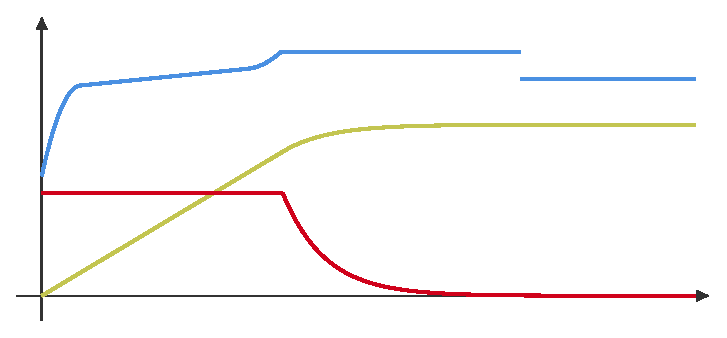
\includegraphics[width=332.25pt,height=145.5pt]{images/image_cccv}};
%Straight Lines [id:da8771255477316724] 
\draw [color={rgb, 255:red, 155; green, 155; blue, 155 }  ,draw opacity=1 ] [dash pattern={on 4.5pt off 4.5pt}]  (422,228.5) -- (422,360) ;
%Shape: Circle [id:dp0014709299474531257] 
\draw  [fill={rgb, 255:red, 255; green, 255; blue, 255 }  ,fill opacity=1 ] (268,203) .. controls (268,201.9) and (268.9,201) .. (270,201) .. controls (271.1,201) and (272,201.9) .. (272,203) .. controls (272,204.1) and (271.1,205) .. (270,205) .. controls (268.9,205) and (268,204.1) .. (268,203) -- cycle ;
%Shape: Circle [id:dp8257690320080588] 
\draw  [fill={rgb, 255:red, 255; green, 255; blue, 255 }  ,fill opacity=1 ] (268,267) .. controls (268,265.9) and (268.9,265) .. (270,265) .. controls (271.1,265) and (272,265.9) .. (272,267) .. controls (272,268.1) and (271.1,269) .. (270,269) .. controls (268.9,269) and (268,268.1) .. (268,267) -- cycle ;
%Straight Lines [id:da48605435215358694] 
\draw [color={rgb, 255:red, 74; green, 144; blue, 226 }  ,draw opacity=1 ][line width=1.5]  [dash pattern={on 1.69pt off 2.76pt}]  (422,207.7) -- (422,217.2) ;
%Straight Lines [id:da6398477641060736] 
\draw    (272,399) -- (420,399) ;
\draw [shift={(422,399)}, rotate = 180] [color={rgb, 255:red, 0; green, 0; blue, 0 }  ][line width=0.75]    (10.93,-3.29) .. controls (6.95,-1.4) and (3.31,-0.3) .. (0,0) .. controls (3.31,0.3) and (6.95,1.4) .. (10.93,3.29)   ;
\draw [shift={(270,399)}, rotate = 0] [color={rgb, 255:red, 0; green, 0; blue, 0 }  ][line width=0.75]    (10.93,-3.29) .. controls (6.95,-1.4) and (3.31,-0.3) .. (0,0) .. controls (3.31,0.3) and (6.95,1.4) .. (10.93,3.29)   ;
%Straight Lines [id:da7717485329022031] 
\draw    (118.5,399) -- (268,399) ;
\draw [shift={(270,399)}, rotate = 180] [color={rgb, 255:red, 0; green, 0; blue, 0 }  ][line width=0.75]    (10.93,-3.29) .. controls (6.95,-1.4) and (3.31,-0.3) .. (0,0) .. controls (3.31,0.3) and (6.95,1.4) .. (10.93,3.29)   ;
\draw [shift={(116.5,399)}, rotate = 0] [color={rgb, 255:red, 0; green, 0; blue, 0 }  ][line width=0.75]    (10.93,-3.29) .. controls (6.95,-1.4) and (3.31,-0.3) .. (0,0) .. controls (3.31,0.3) and (6.95,1.4) .. (10.93,3.29)   ;
%Straight Lines [id:da8998950689600032] 
\draw    (116,394) -- (116,404) ;
%Straight Lines [id:da17048346486898192] 
\draw    (270,394) -- (270,404) ;
%Straight Lines [id:da8039553388960854] 
\draw    (422,394) -- (422,404) ;
%Straight Lines [id:da2911914982770165] 
\draw [color={rgb, 255:red, 74; green, 144; blue, 226 }  ,draw opacity=1 ]   (78,124) -- (103,124) ;
%Straight Lines [id:da500593174587459] 
\draw [color={rgb, 255:red, 208; green, 2; blue, 27 }  ,draw opacity=1 ]   (78,144) -- (103,144) ;
%Straight Lines [id:da47080918502581004] 
\draw [color={rgb, 255:red, 195; green, 197; blue, 81 }  ,draw opacity=1 ]   (78,164) -- (103,164) ;

%Straight Lines [id:da7924785218065409] 
\draw [color={rgb, 255:red, 155; green, 155; blue, 155 }  ,draw opacity=1 ] [dash pattern={on 4.5pt off 4.5pt}]  (117,249) -- (533,249) ;

% Text Node
\draw (106,117.4) node [anchor=north west][inner sep=0.75pt]  [font=\footnotesize]  {$U_{\mathrm{B}}( t)$};
% Text Node
\draw (106,137.4) node [anchor=north west][inner sep=0.75pt]  [font=\footnotesize]  {$I_{\mathrm{B}}( t)$};
% Text Node
\draw (106,157.4) node [anchor=north west][inner sep=0.75pt]  [font=\footnotesize]  {$Q_{\mathrm{B}}( t)$};
% Text Node
\draw (547,352.4) node [anchor=north west][inner sep=0.75pt]  [font=\footnotesize]  {$t$};
% Text Node
\draw (142,382) node [anchor=north west][inner sep=0.75pt]  [font=\footnotesize] [align=left] {Constant current};
% Text Node
\draw (294,382) node [anchor=north west][inner sep=0.75pt]  [font=\footnotesize] [align=left] {Constant voltage};
% Text Node
\draw (102,363.4) node [anchor=north west][inner sep=0.75pt]  [font=\footnotesize]  {$0$};
% Text Node
\draw (84.5,242.4) node [anchor=north west][inner sep=0.75pt]  [font=\footnotesize]  {$Q_{\mathrm{tot}}$};
% Text Node
\draw (87,198.4) node [anchor=north west][inner sep=0.75pt]  [font=\scriptsize]  {$U_{\mathrm{full}}$};
% Text Node
\draw (97.2,287.4) node [anchor=north west][inner sep=0.75pt]  [font=\scriptsize]  {$I_{\mathrm{C}}$};
% Text Node
\draw (263,362.4) node [anchor=north west][inner sep=0.75pt]  [font=\footnotesize]  {$t_{\mathrm{C}}$};
% Text Node
\draw (400,362.4) node [anchor=north west][inner sep=0.75pt]  [font=\footnotesize]  {$t_{\mathrm{C}} +t_{\mathrm{V}}$};
% Text Node
\draw (60.5,259.4) node [anchor=north west][inner sep=0.75pt]  [font=\footnotesize]  {$Q_{\mathrm{B}}( t_{\mathrm{CC}})$};


\end{tikzpicture}






	\caption{An example of the behavior the battery voltage $U_\mathrm{B}(t)$, battery current $I_\mathrm{B}(t)$ and battery charge $Q_\mathrm{B}(t)$ of a $\mathrm{LiFePO}_4$ battery when it is charged with a constant current $I_\mathrm{C}$ and then with a constant voltage $U_\mathrm{full}$ over a longer period of time. At $t_\mathrm{C} + t_\mathrm{V}$ the battery charger switches from $U_\mathrm{full}$ to $U_\mathrm{float}$ to keep the battery in a fully charged state. (Recreated from: \cite{Notten:2005, Sterner:2017, Liu:2020})}
	\label{fig:tikz_cccv_curve}
\end{figure} 

With the \emph{charge difference} $\Delta Q = Q_\mathrm{tot} - Q_\mathrm{B}(t_\mathrm{C})$ and the model proposed in \cite{Liu:2020}, the battery charge can be written as a function of the charging time as follows: 
\begin{equation} \label{eq:battery_charge_cases}
\centering
		Q_\mathrm{B}(t) =
  		\begin{cases}
   			I_\mathrm{C} \, t \text{,} & \text{for } 0\mathrm{h} \leq t < t_\mathrm{C} 
			\\
    		\Delta Q \left( 1 - \exp \left( -\dfrac{t - t_\mathrm{C}}{\tau_\mathrm{B}} \right) \right) + I_\mathrm{C} \, t_\mathrm{C}\text{,} & \text{for } t_\mathrm{C} \leq t < t_\mathrm{C} + t_\mathrm{V} \text{.}
  		\end{cases}
\end{equation}
It is assumed that $Q_\mathrm{B}(t)$ is continuously differentiable for all points in time. Based on this assumption, the model for the charging current results from the time derivative: 
\begin{equation} \label{current_cases}
\dfrac{\mathrm{d}Q_\mathrm{B}(t)}{\mathrm{d}t} = 
	\left\{\begin{array}{ll}
		I_\mathrm{C}\text{,} & \text{for } 0\mathrm{h} \leq t < t_\mathrm{C} \\[8pt]
		\dfrac{\Delta Q}{\tau_\mathrm{B}} \exp \left( -\dfrac{t - t_\mathrm{C}}{\tau_\mathrm{B}} \right)\text{,} & \text{for } t_\mathrm{C} \leq t < t_\mathrm{C} + t_\mathrm{V}
 	\end{array}\right\} = I_\mathrm{B}(t) \text{.}
\end{equation}
If it is further assumed that $I_\mathrm{B}(t)$ is continuous for all points in time -- therefore does not drop at the point in time $t_\mathrm{C}$ -- the \emph{time constant} $\tau_\mathrm{B}$ in $\left(\mathrm{h}\right)$ of a battery can be obtained from:
\begin{equation}\label{eq:tau_battery}
	\centering
	\tau_\mathrm{B} = \dfrac{\Delta Q}{I_\mathrm{C}}\text{.}
\end{equation}
If -- in the course of the charge experiment -- it can be shown that the second assumption is correct, then the first assumption follows according to \cite{Taschner:2014}.
	
Like the discharge experiment, this experiment is also carried out at $\vartheta_\mathrm{A} = 25^\circ \mathrm{C}$. The $\mathrm{LiFePO}_4$ battery, however, is initially fully discharged ($\mathrm{SOC}_{1} = 0$) and the charging experiment is repeated for the desired number of measuring points $N_{\mathrm{MP}}$ until it is fully charged ($\mathrm{SOC}_{N_\mathrm{MP}} = 1$) \cite{Rahmoun:2012, Hentunen:2014, Gurjer:2019}.

The corresponding measurement setup can be seen in the figure \ref{fig:tikz_experiment_2}. For the currents $I_\mathrm{Ch1}$ and $I_\mathrm{Ch2}$ the same applies as in the discharge experiment since they are small compared to the \emph{battery charger current} $I_\mathrm{BC}$ in $\left(\mathrm{A}\right)$ \cite{Schrufer:2014}.
\begin{figure}[h!]
	\centering
	

\tikzset{every picture/.style={line width=0.75pt}} %set default line width to 0.75pt        

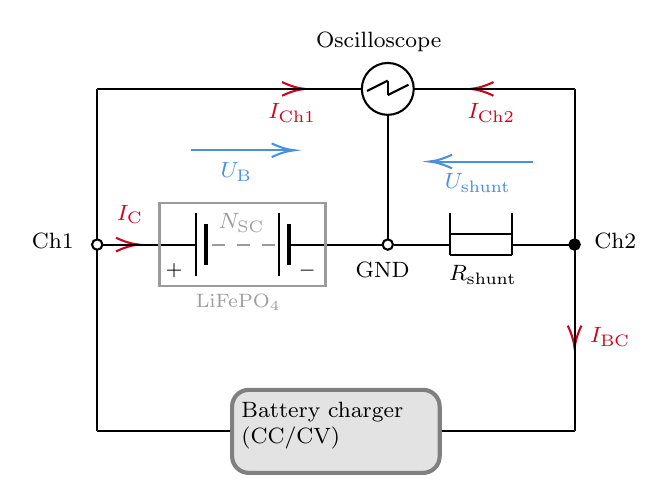
\begin{tikzpicture}[x=0.75pt,y=0.75pt,yscale=-1,xscale=1]
%uncomment if require: \path (0,748); %set diagram left start at 0, and has height of 748

%Straight Lines [id:da030470885996142894] 
\draw [color={rgb, 255:red, 208; green, 2; blue, 27 }  ,draw opacity=1 ]   (360,170) ;
\draw [shift={(360,170)}, rotate = 180] [color={rgb, 255:red, 208; green, 2; blue, 27 }  ,draw opacity=1 ][line width=0.75]    (10.93,-3.29) .. controls (6.95,-1.4) and (3.31,-0.3) .. (0,0) .. controls (3.31,0.3) and (6.95,1.4) .. (10.93,3.29)   ;
%Straight Lines [id:da3824823238969528] 
\draw [color={rgb, 255:red, 208; green, 2; blue, 27 }  ,draw opacity=1 ]   (570,205) -- (570,218) ;
\draw [shift={(570,220)}, rotate = 270] [color={rgb, 255:red, 208; green, 2; blue, 27 }  ,draw opacity=1 ][line width=0.75]    (10.93,-3.29) .. controls (6.95,-1.4) and (3.31,-0.3) .. (0,0) .. controls (3.31,0.3) and (6.95,1.4) .. (10.93,3.29)   ;
%Straight Lines [id:da5182691574210985] 
\draw    (340,260) -- (407.5,260) ;
%Straight Lines [id:da26468661252829784] 
\draw    (502.5,260) -- (570,260) ;
%Rounded Rect [id:dp15109738720083965] 
\draw  [color={rgb, 255:red, 128; green, 128; blue, 128 }  ,draw opacity=1 ][fill={rgb, 255:red, 227; green, 227; blue, 227 }  ,fill opacity=1 ][line width=1.5]  (405,248) .. controls (405,243.58) and (408.58,240) .. (413,240) -- (497,240) .. controls (501.42,240) and (505,243.58) .. (505,248) -- (505,272) .. controls (505,276.42) and (501.42,280) .. (497,280) -- (413,280) .. controls (408.58,280) and (405,276.42) .. (405,272) -- cycle ;
%Straight Lines [id:da04571217565366692] 
\draw [color={rgb, 255:red, 208; green, 2; blue, 27 }  ,draw opacity=1 ]   (535,95) -- (522,95) ;
\draw [shift={(520,95)}, rotate = 360] [color={rgb, 255:red, 208; green, 2; blue, 27 }  ,draw opacity=1 ][line width=0.75]    (10.93,-3.29) .. controls (6.95,-1.4) and (3.31,-0.3) .. (0,0) .. controls (3.31,0.3) and (6.95,1.4) .. (10.93,3.29)   ;
%Straight Lines [id:da286200132644544] 
\draw    (342,170) -- (370,170) ;
%Straight Lines [id:da17958881147308237] 
\draw    (450.5,170) -- (477.5,170) ;
%Straight Lines [id:da5043205087506204] 
\draw [color={rgb, 255:red, 208; green, 2; blue, 27 }  ,draw opacity=1 ]   (425,95) -- (438,95) ;
\draw [shift={(440,95)}, rotate = 180] [color={rgb, 255:red, 208; green, 2; blue, 27 }  ,draw opacity=1 ][line width=0.75]    (10.93,-3.29) .. controls (6.95,-1.4) and (3.31,-0.3) .. (0,0) .. controls (3.31,0.3) and (6.95,1.4) .. (10.93,3.29)   ;
%Straight Lines [id:da8819726416071505] 
\draw [line width=0.75]    (387.5,155) -- (387.5,185) ;
%Straight Lines [id:da22364644407030787] 
\draw [color={rgb, 255:red, 155; green, 155; blue, 155 }  ,draw opacity=1 ] [dash pattern={on 4.5pt off 4.5pt}]  (425.5,170) -- (390.5,170) ;
%Straight Lines [id:da8171048209291414] 
\draw [line width=1.5]    (392.5,160) -- (392.5,180) ;
%Straight Lines [id:da3784748951709651] 
\draw [line width=0.75]    (427.5,155) -- (427.5,185) ;
%Straight Lines [id:da23453075334713613] 
\draw [line width=1.5]    (432.5,160) -- (432.5,180) ;
%Straight Lines [id:da7174267672251604] 
\draw    (387.5,170) -- (370.5,170) ;
%Straight Lines [id:da8824908036219616] 
\draw    (449.5,170) -- (432.5,170) ;
%Shape: Rectangle [id:dp6355233140968859] 
\draw  [color={rgb, 255:red, 155; green, 155; blue, 155 }  ,draw opacity=1 ] (450,150) -- (450,190) -- (370,190) -- (370,150) -- cycle ;
%Shape: Circle [id:dp4046675137999993] 
\draw   (477.5,170) .. controls (477.5,168.62) and (478.62,167.5) .. (480,167.5) .. controls (481.38,167.5) and (482.5,168.62) .. (482.5,170) .. controls (482.5,171.38) and (481.38,172.5) .. (480,172.5) .. controls (478.62,172.5) and (477.5,171.38) .. (477.5,170) -- cycle ;
%Shape: Circle [id:dp8699232468402804] 
\draw   (337.5,170) .. controls (337.5,168.62) and (338.62,167.5) .. (340,167.5) .. controls (341.38,167.5) and (342.5,168.62) .. (342.5,170) .. controls (342.5,171.38) and (341.38,172.5) .. (340,172.5) .. controls (338.62,172.5) and (337.5,171.38) .. (337.5,170) -- cycle ;
%Straight Lines [id:da0932789662810869] 
\draw    (340,95) -- (340,167.5) ;
%Straight Lines [id:da7259313392072295] 
\draw    (340,95) -- (467.5,95) ;
%Straight Lines [id:da7181235672344906] 
\draw [color={rgb, 255:red, 74; green, 144; blue, 226 }  ,draw opacity=1 ]   (385,124.57) -- (433,124.57) ;
\draw [shift={(435,124.57)}, rotate = 180] [color={rgb, 255:red, 74; green, 144; blue, 226 }  ,draw opacity=1 ][line width=0.75]    (10.93,-3.29) .. controls (6.95,-1.4) and (3.31,-0.3) .. (0,0) .. controls (3.31,0.3) and (6.95,1.4) .. (10.93,3.29)   ;
%Shape: Circle [id:dp9954794574731103] 
\draw   (467.5,95) .. controls (467.5,88.1) and (473.1,82.5) .. (480,82.5) .. controls (486.9,82.5) and (492.5,88.1) .. (492.5,95) .. controls (492.5,101.9) and (486.9,107.5) .. (480,107.5) .. controls (473.1,107.5) and (467.5,101.9) .. (467.5,95) -- cycle ;
%Straight Lines [id:da04493405460274014] 
\draw    (470,96) -- (480,91) ;
%Straight Lines [id:da3033269159759058] 
\draw    (480,91) -- (480,98) ;
%Straight Lines [id:da8245646456208624] 
\draw    (480,98) -- (490,93) ;

%Straight Lines [id:da664654756239323] 
\draw    (340,172.5) -- (340,260) ;
%Straight Lines [id:da020631229787501093] 
\draw    (570,170) -- (570,260) ;
%Straight Lines [id:da42439143356479936] 
\draw    (492.5,95) -- (570,95) ;
%Straight Lines [id:da8878395010937925] 
\draw    (540,175) -- (540,165) ;
%Straight Lines [id:da5068559712609504] 
\draw    (510,175) -- (510,165) ;
%Straight Lines [id:da17027035780260014] 
\draw    (510,175) -- (540,175) ;
%Straight Lines [id:da7267594413628695] 
\draw    (510,165) -- (540,165) ;
%Straight Lines [id:da6452827698871475] 
\draw    (510,155) -- (510,165) ;
%Straight Lines [id:da9670069496965643] 
\draw    (540,155) -- (540,165) ;
%Shape: Circle [id:dp9967471299276287] 
\draw  [fill={rgb, 255:red, 0; green, 0; blue, 0 }  ,fill opacity=1 ] (570,167.5) .. controls (571.38,167.5) and (572.5,168.62) .. (572.5,170) .. controls (572.5,171.38) and (571.38,172.5) .. (570,172.5) .. controls (568.62,172.5) and (567.5,171.38) .. (567.5,170) .. controls (567.5,168.62) and (568.62,167.5) .. (570,167.5) -- cycle ;
%Straight Lines [id:da6778579527436412] 
\draw    (540,170) -- (570,170) ;
%Straight Lines [id:da9391362233033829] 
\draw    (483,170) -- (510,170) ;
%Straight Lines [id:da8151174249515367] 
\draw    (480,107.5) -- (480,167.5) ;
%Straight Lines [id:da4990891660653225] 
\draw [color={rgb, 255:red, 74; green, 144; blue, 226 }  ,draw opacity=1 ]   (550,130) -- (502,130) ;
\draw [shift={(500,130)}, rotate = 360] [color={rgb, 255:red, 74; green, 144; blue, 226 }  ,draw opacity=1 ][line width=0.75]    (10.93,-3.29) .. controls (6.95,-1.4) and (3.31,-0.3) .. (0,0) .. controls (3.31,0.3) and (6.95,1.4) .. (10.93,3.29)   ;
%Straight Lines [id:da37596819517946445] 
\draw    (570,95) -- (570,167.5) ;

% Text Node
\draw (576,208.4) node [anchor=north west][inner sep=0.75pt]  [font=\footnotesize,color={rgb, 255:red, 208; green, 2; blue, 27 }  ,opacity=1 ]  {$I_{\mathrm{BC}}$};
% Text Node
\draw (348,149.4) node [anchor=north west][inner sep=0.75pt]  [font=\footnotesize,color={rgb, 255:red, 208; green, 2; blue, 27 }  ,opacity=1 ]  {$I_{\mathrm{C}}$};
% Text Node
\draw (408,244.5) node [anchor=north west][inner sep=0.75pt]  [font=\footnotesize] [align=left] {Battery charger\\(CC/CV)};
% Text Node
\draw (386,192.4) node [anchor=north west][inner sep=0.75pt]  [font=\scriptsize,color={rgb, 255:red, 0; green, 0; blue, 0 }  ,opacity=1 ]  {$\mathrm{\textcolor[rgb]{0.61,0.61,0.61}{LiFePO}\textcolor[rgb]{0.61,0.61,0.61}{_{4}}}$};
% Text Node
\draw (435.5,177.4) node [anchor=north west][inner sep=0.75pt]  [font=\scriptsize]  {$-$};
% Text Node
\draw (371.5,177.4) node [anchor=north west][inner sep=0.75pt]  [font=\scriptsize]  {$+$};
% Text Node
\draw (397,153.4) node [anchor=north west][inner sep=0.75pt]  [font=\footnotesize,color={rgb, 255:red, 155; green, 155; blue, 155 }  ,opacity=1 ]  {$N_{\mathrm{SC}}$};
% Text Node
\draw (398,128.97) node [anchor=north west][inner sep=0.75pt]  [font=\footnotesize,color={rgb, 255:red, 74; green, 144; blue, 226 }  ,opacity=1 ]  {$U_{\mathrm{B}}$};
% Text Node
\draw (421,100.4) node [anchor=north west][inner sep=0.75pt]  [font=\footnotesize,color={rgb, 255:red, 208; green, 2; blue, 27 }  ,opacity=1 ]  {$I_{\mathrm{Ch} 1}$};
% Text Node
\draw (444,66) node [anchor=north west][inner sep=0.75pt]  [font=\footnotesize] [align=left] {Oscilloscope};
% Text Node
\draw (508,178.4) node [anchor=north west][inner sep=0.75pt]  [font=\footnotesize]  {$R_{\mathrm{shunt}}$};
% Text Node
\draw (506,134.4) node [anchor=north west][inner sep=0.75pt]  [font=\footnotesize,color={rgb, 255:red, 74; green, 144; blue, 226 }  ,opacity=1 ]  {$U_{\mathrm{shunt}}$};
% Text Node
\draw (517,100.4) node [anchor=north west][inner sep=0.75pt]  [font=\footnotesize,color={rgb, 255:red, 208; green, 2; blue, 27 }  ,opacity=1 ]  {$I_{\mathrm{Ch} 2}$};
% Text Node
\draw (463,177) node [anchor=north west][inner sep=0.75pt]  [font=\footnotesize] [align=left] {GND};
% Text Node
\draw (578,163) node [anchor=north west][inner sep=0.75pt]  [font=\footnotesize] [align=left] {Ch2};
% Text Node
\draw (307,163) node [anchor=north west][inner sep=0.75pt]  [font=\footnotesize] [align=left] {Ch1};


\end{tikzpicture}

	\caption{Measurement setup for the charge experiment.}
	\label{fig:tikz_experiment_2}
\end{figure}
Based on the figure \ref{fig:tikz_experiment_2}, the actual charging current $I_\mathrm{C}$ can be calculated with the equation (\ref{eq:i_c_real}).
\begin{equation}\label{eq:i_c_real}
	\centering
I_\mathrm{C} = -\dfrac{U_\mathrm{shunt}}{R_\mathrm{shunt}} - I_\mathrm{Ch1} - I_\mathrm{Ch2}
\end{equation}

Identical to the discharge experiment, the battery's open-circuit voltage $U_{0, \mathrm{C}}(\mathrm{SOC}_n)$ in $\left(\mathrm{V}\right)$ is measured with Ch1. The battery is then charged using a suitable battery charger in (CC/CV) mode with a set $I_{\mathrm C}$, $I_\mathrm{min}$, $U_\mathrm{full}$ and $U_\mathrm{float}$. This is done for the time interval $\Delta t_{\mathrm{C}}$ until the new measuring point $\mathrm{SOC}_{n+1}$ is reached. At the point in time when the battery charger is switched on, the voltage rise $\Delta U_{\mathrm C}(\mathrm{SOC}_n)$ is measured with Ch1 and the voltage drop $U_\mathrm{shunt}(\mathrm{SOC}_n)$ with Ch2. After the charge process for $\Delta t_{\mathrm{C}}$ has been completed, the battery must remain idle for $t_\mathrm{rest}$ until the open-circuit voltage has reached an end value (compare to figure \ref{fig:tikz_pc_pd_battery_curve}). When this value is reached, the measurements can be repeated for $\mathrm{SOC}_{n + 1}$ \cite{Rahmoun:2012, Hentunen:2014, Gurjer:2019}. Based on the previously introduced model $\Delta U_{\mathrm C}(\mathrm{SOC}_{N_\mathrm{MP}})$ cannot be obtained. However, by performing the experiment on a commercially available $\mathrm{LiFePO}_4$ battery, it was found that for longer resting periods $t_\mathrm{rest}$, of up to a few hours, it accepts small charging currents $I_{\mathrm C}$ for a short intervall $\Delta t_\mathrm{C}$ even for $\mathrm{SOC}_{N_\mathrm{MP}}$. It is assumed that this is the consequence of the slow -- almost exponential -- decrease of $U_{0, \mathrm{C}}(\mathrm{SOC}_{_\mathrm{MP}})$ (compare to figure \ref{fig:tikz_pc_pd_battery_curve}) \cite{Kurzweil:2018}. In this case, the equation (\ref{eq:battery_voltage}) is not equal to $U_{\mathrm{full}}$ anymore.

To confirm the previously made assumption that $I_{\mathrm C}(t)$ is continuous for all points in time, it is measured with Ch2 and calculated by using the equation (\ref{eq:i_c_real}) \cite{Notten:2005, Mertens:2015, Sterner:2017, Kurzweil:2018, Liu:2020}. 

The time interval $\Delta t_{\mathrm{C}}$ and the measuring points are calculated -- base on the Coulomb counting method -- as shown below \cite{He:2011, Wehbe:2015, Nejad:2016, Kurzweil:2018, Li:2018}:
\begin{equation} \label{eq:delta_t_C}
	\centering
	\Delta t_{\mathrm{C}} = \dfrac{ Q_\mathrm{tot}}{\eta_\mathrm{C} \, I_\mathrm{C} \left( N_\mathrm{MP} - 1 \right)} \text{.}
\end{equation}
\begin{equation} \label{eq:SOC_n_plus_1}
	\centering
	\mathrm{SOC}_{n + 1} = \mathrm{SOC}_{n} + \dfrac{\eta_\mathrm{C} \, I_\mathrm{C}}{Q_\mathrm{tot}} \, \Delta t_{\mathrm{C}} \text{.}
\end{equation}

Similar to $R_{e,\mathrm{D}}$, $R_{e,\mathrm{C}}$ can be obtained -- by using the equations (\ref{eq:r_0_c}) and (\ref{eq:i_c_real}) -- from \cite{Rahmoun:2012, Hentunen:2014, Kurzweil:2018, Gurjer:2019}:
\begin{equation}\label{eq:r_0_c_soc}
	\centering
	R_{\mathrm{e,C}}(\mathrm{SOC}_n) = \left|-\dfrac{\Delta U_{\mathrm C}(\mathrm{SOC}_n)}{\dfrac{U_\mathrm{shunt}(\mathrm{SOC}_n)}{R_\mathrm{shunt}} + I_\mathrm{Ch1} + I_\mathrm{Ch2}}\right| \text{.}
\end{equation}

Due to the hysteresis effects of the open-circuit voltage $U_0(\mathrm{SOC}_n)$ mentioned in \cite{Hentunen:2014, Wehbe:2015, Gurjer:2019, Saldana:2019}, the battery voltage in the equation (\ref{eq:battery_voltage}) must be adapted to the so-called \emph{zero-state hysteresis model}:

\begin{equation} \label{eq:battery_voltage_adapted}
	\centering
		U_\mathrm{B}(\mathrm{SOC}_n) =
  		\begin{cases}
   			U_0 (\mathrm{SOC}_n)+ \dfrac{c_{\mathrm{B}}}{2} - R_{\mathrm{e,D}}(\mathrm{SOC}_n) \, I_\mathrm{D}\text{,} \\ \text{when discharging the battery} \\[8pt]
    		U_0(\mathrm{SOC}_n) + \dfrac{c_{\mathrm{B}}}{2} + R_{\mathrm{e,C}}(\mathrm{SOC}_n) \, I_\mathrm{C}\text{,} \\\text{when charging the battery,}
  		\end{cases}
	\end{equation} 
with: 
\begin{equation} \label{eq:U_0}
	\centering
	U_0(\mathrm{SOC}_n) = \dfrac{U_{0,\mathrm{D}}(\mathrm{SOC}_n) + U_{0,\mathrm{C}}(\mathrm{SOC}_n)}{2}\text{,}
\end{equation}
and $c_{\mathrm{B}}$ depending on the sign of $I_\mathrm{B}$:
\begin{equation} \label{eq:c_B}
	\centering
		c_{\mathrm{B}} =
  		\begin{cases}
   			\left| U_{0, \mathrm{C}}(\mathrm{SOC}_n) - U_{0, \mathrm{D}}(\mathrm{SOC}_n) \right| \cdot (-1) \text{,} & \text{for } I_\mathrm{B} > 0\mathrm{A} \\
			0\text{,} & \text{for } I_\mathrm{B} = 0\mathrm{A} \\
			\left| U_{0, \mathrm{C}}(\mathrm{SOC}_n) - U_{0, \mathrm{D}}(\mathrm{SOC}_n) \right| \text{,} & \text{for } I_\mathrm{B} < 0\mathrm{A}\text{.}
  		\end{cases}
	\end{equation} 



\subsection{Cable losses}
Cables are used to distribute the generated electrical energy in the self-sufficient voice communication system. The transport of the \emph{electrical charge} $Q$ in $\left( \mathrm{As} \right)$ in a cable, however, causes electrical losses which have to be considered with: 
	\begin{equation} \label{eq:p_cable}
	\centering
		 P_\mathrm{loss}(\vartheta_\mathrm{A}) = \left(\dfrac{\mathrm d Q(A)}{\mathrm d t}\right)^2 R_\mathrm{cable}(\vartheta_\mathrm{A}) \text{.}
	\end{equation}
$I(A) = \mathrm d Q(A) / \mathrm d t$ represents the time throughput rate of the electrical charge shifted in a directed manner through the \emph{cross-sectional area} $A$ in $\left( \mathrm{mm}^2 \right)$ of a cable. This corresponds to the electrical current $I$ in $\left( \mathrm{A} \right)$ at the area $A$. The second factor $R_\mathrm{cable}(\vartheta_\mathrm{A})$ in $\left( \Omega \right)$ is the \emph{cable resistance} depending on the ambient temperature $\vartheta_\mathrm{A}$. It can be calculated with the equation (\ref{eq:r_cable}), where $l$ in $\left( \mathrm m \right)$ is the \emph{length} of the cable, $\varrho$ in $\left(\Omega \mathrm{mm}^2\mathrm{m}^{-1}\right)$ is the \emph{specific resistance} and $\alpha$ in $\left( ^\circ \mathrm{C}^{-1} \right)$ is the \emph{temperature coefficient} of the material the cable is made of. $\vartheta_\mathrm{ref}$ in $\left( ^\circ \mathrm{C} \right)$ is the temperature for which $\varrho$ applies.
	\begin{equation} \label{eq:r_cable}
	\centering
		 R_\mathrm{cable}(\vartheta_\mathrm{A}) = \dfrac{\varrho \, l}{A} \, \left[1 + \alpha \left( \vartheta_\mathrm{A} - \vartheta_\mathrm{ref}\right) \right]
	\end{equation}
For example, for $\vartheta_\mathrm{ref} = 20^\circ \mathrm{C}$ copper has a specific resistance of $\varrho_\mathrm{Cu,20} = 0,01673 \Omega \mathrm{mm}^2\mathrm{m}^{-1}$ with a temprature coefficient of $\alpha = {4,3 \cdot 10^{-3}}^\circ \mathrm{C}^{-1}$ \cite{Gerhard-Fasching:2005, Prechtl:2006}. Cable heating by solar radiation is neglected due to the complexity of the subject. 

\subsection{Martian application}
With regard to the usability of the modeled energy distribution for a self-sufficient voice communication system on the surface of Mars, roughly speaking, two main components have to be examined more closely. Namely the PV generator and the $\mathrm{LiFePO}_4$ battery.

Since Mars, with an average distance of $1,524\mathrm{AU}$, is further away from the Sun than the Earth, the solar irradiance $E_\mathrm{S,M}$ in $\left(\mathrm{Wm^{-2}}\right)$ at the top of its atmosphere is $56,9\%$ less than that on Earth \cite{Karttunen:2006}: 
\begin{equation} \label{eq:e_sun_mars}
	\centering
	E_{\mathrm{S,M}} = \frac{\Phi_{\mathrm{S}}}{4 \pi \, \left(1,524 \cdot r_{\mathrm{SE}}\right)^2} = \frac{3,845 \cdot 10^{26} \mathrm{W}}{4 \pi \cdot (2,279871539 \cdot 10^{11} \mathrm{m})^2} = 588,66 \frac{\mathrm{W}}{\mathrm{m}^2}\text{.}
\end{equation}
Similar to the solar resource maps introduced in the subsection \ref{sec:solar_irradiation_on_earths_surface}, the Solar irradiance data collected by NASA's Viking Lander VL1, shown in the figures \ref{fig:image_mars_irradiance_mean} to \ref{fig:image_mars_irradiance_orbit}, can be used to calculate the total generator irradiance on the Martian surface, based on the equations (\ref{eq:e_dni}) and (\ref{eq:e_gen_ghi_dni}):
\begin{equation} \label{eq:e_gen_ghi_dni_mars}
	\centering
		E_{\mathrm{G}}(t_\mathrm{S}) = E_{\mathrm{DHI}} \, \dfrac{\cos \theta}{\sin \gamma_\mathrm{S}} + E_{\mathrm{DIFH}} \,\frac{1 + \cos \beta }{2} + E_{\mathrm{GHI}} \, \frac{1 - \cos \beta }{2} \cdot \mathrm{ALB} \text{.}
\end{equation}
\begin{figure}[h!]
	\centering
  	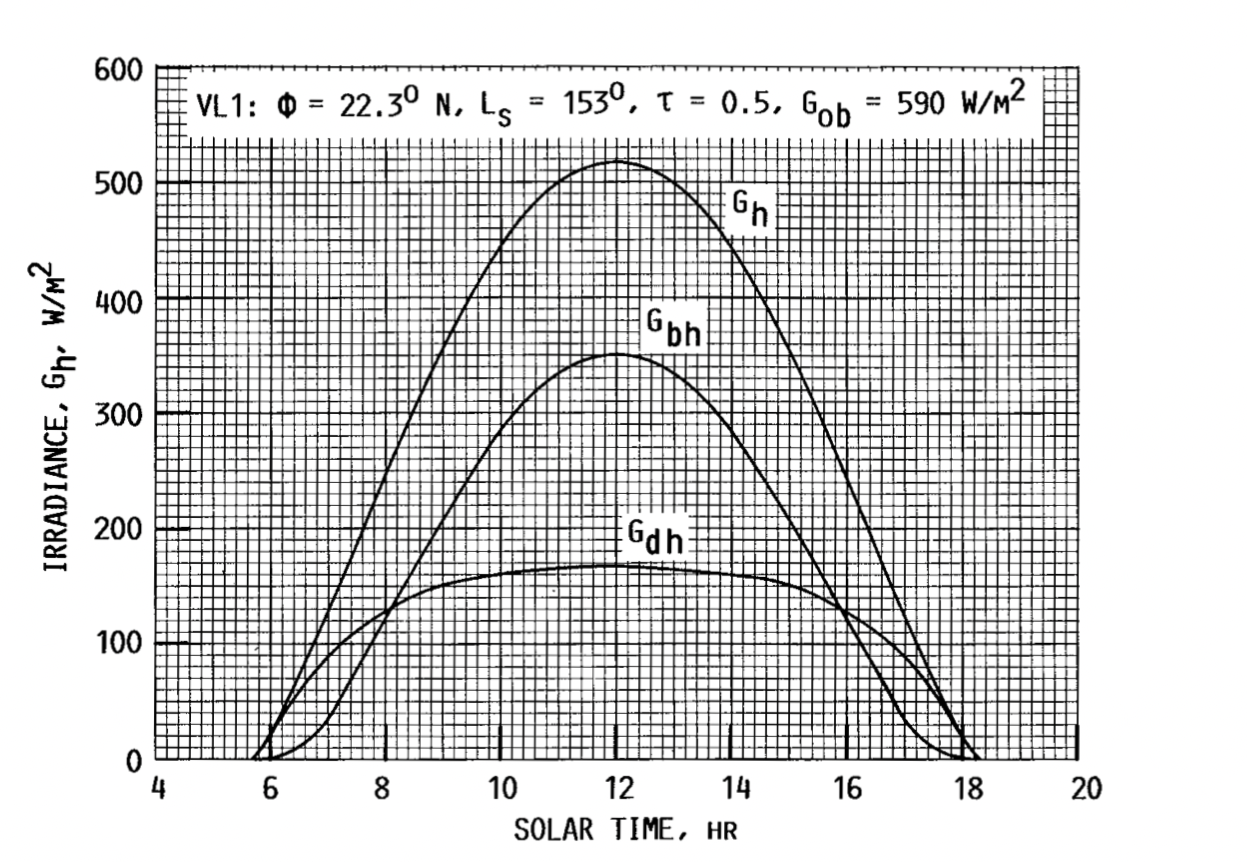
\includegraphics[width = 0.9\textwidth]{images/image_mars_irradiance_mean}
  	\caption{\textit{``Diurnal variation of global $G_\mathrm{h}$, beam $G_\mathrm{bh}$ and diffuse $G_\mathrm{dh}$ irradiance on a horizontal Mars surface at Viking Lander VL1.''} (Image and caption credit: \cite{Appelbaum:1990})}
	\label{fig:image_mars_irradiance_mean}
\end{figure}
The quantities $E_{\mathrm{DHI}}$, $E_{\mathrm{DIFH}}$, $E_{\mathrm{GHI}}$, $\theta$ and $\gamma_\mathrm{S}$ depend on the solar time $t_\mathrm{S}$. As a first approximation, the albedo value $\mathrm{ALB} = 0,25$ can be used. This value represents the mean albedo of Mars \cite{Grayzeck:2020}. In the article \cite{Appelbaum:1990} the authors further state that the albedo of the Martian surface varies in the range of $0,1$ to $0,4$.

The data presented in the figures \ref{fig:image_mars_irradiance_mean} to \ref{fig:image_mars_irradiance_orbit}, however, only applies for the Martian latitude $\phi \ \widehat{=} \ \varphi = 22,3^\circ \, \mathrm{N}$. Figure \ref{fig:image_mars_irradiance_mean} shows the diurnal variation of $E_{\mathrm{DHI}} \ \widehat{=} \ G_\mathrm{bh}$, $E_{\mathrm{DIFH}} \ \widehat{=} \ G_\mathrm{dh}$ and $E_{\mathrm{GHI}} \ \widehat{=} \ G_\mathrm{h}$ on the Martian surface. The quantities $L_\mathrm{S}$, $\tau$ and $G_\mathrm{ob}$ are the areocentric longitude, the optical depth and the beam irradiance at the top of the Martian atmosphere. Similar data is shown in the figures \ref{fig:image_mars_irradiance_orbit} and \ref{fig:image_mars_irradiance_opacity}, but here an additional reference is made to the orbit of Mars around the Sun and the opacity of its atmosphere. For example, the latter can be caused by dust storms \cite{Appelbaum:1990}. 
\begin{figure}[h!]
	\centering
  	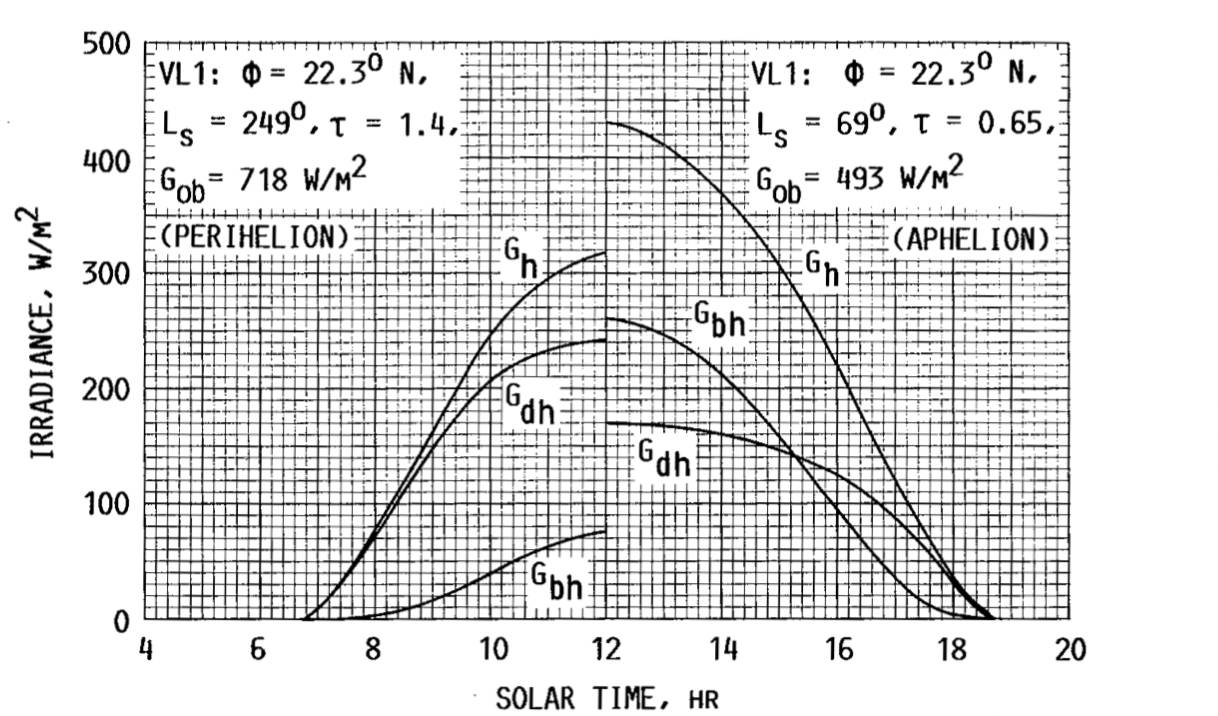
\includegraphics[width = 0.9\textwidth]{images/image_mars_irradiance_orbit}
  	\caption{\textit{``Diurnal variation of global $G_\mathrm{h}$, beam $G_\mathrm{bh}$ and diffuse $G_\mathrm{dh}$ irradiance on a horizontal Mars surface at Viking Lander VL1.''} (Image and caption credit: \cite{Appelbaum:1990})}
	\label{fig:image_mars_irradiance_orbit}
\end{figure}
\begin{figure}[h!]
	\centering
  	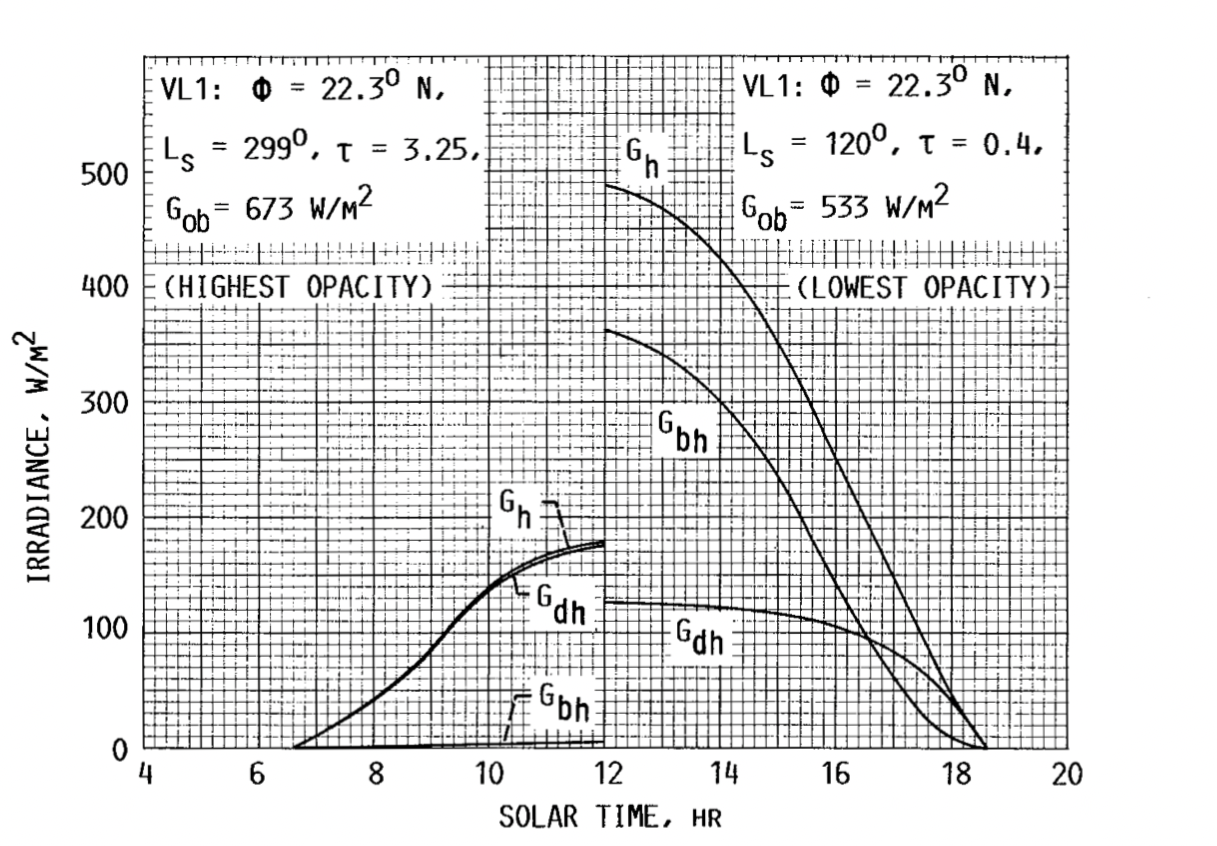
\includegraphics[width = 0.9\textwidth]{images/image_mars_irradiance_opacity}
  	\caption{\textit{``Diurnal variation of global $G_\mathrm{h}$, beam $G_\mathrm{bh}$ and diffuse $G_\mathrm{dh}$ irradiance on a horizontal Mars surface at Viking Lander VL1.''} (Image and caption credit: \cite{Appelbaum:1990})}
	\label{fig:image_mars_irradiance_opacity}
\end{figure}

The angles $\theta$ and $\gamma_\mathrm{S}$ can be calculated with the equations introduced in the subsections \ref{sec:angular_relationships} and \ref{sec:energy_yield}. For these, however, the local latitude $\varphi$, the Sun's declination $\delta$ and the solar time $t_\mathrm{S}$ on Mars must be known. On Mars, the maximum values of $\delta$ are $-25,19^\circ$ and $25,19^\circ$ and the duration of one day is $24,6597\mathrm{h}$ \cite{Grayzeck:2020}. It is noted, that the equations (\ref{eq:delta}) and (\ref{eq:solar_time}) cannot be used to calculate $\delta$ and $t_\mathrm{S}$.

In order to get the same energy yield with a PV generator on Mars as on Earth, this can be achieved in two ways. Based on the equation (\ref{eq:radiation_flux}), and if it is assumed that the PV cell temperatures of the PV generator on Earth and Mars are equal ($\vartheta_\mathrm{C,E} = \vartheta_\mathrm{C,M}$), the radiation flux onto the energy-converting area $A_\mathrm{PV,E}$ of the PV generator on Earth is equal to the radiation flux onto the energy-converting area $A_\mathrm{PV,M}$ of the PV generator on Mars, when the following equation applies:
\begin{equation} \label{eq:pv_area_comparison}
	\centering
		A_{\mathrm{PV,M}} = A_{\mathrm{PV,E}} \, \dfrac{E_{\mathrm{G,E}}}{E_{\mathrm{G,M}}}\text{,} \quad \text{for } \vartheta_\mathrm{C,E} = \vartheta_\mathrm{C,M} \text{.}
\end{equation}
Therefore, a self-sufficient voice communication system with a PV generator area $A_{\mathrm{PV,E}}$ and, for example, the requirement of an annual average irradiance $E_{\mathrm{G,E}}$ to operate on Earth, would require an area $A_{\mathrm{PV,M}}$ if there is an annual avarege irradiance $E_{\mathrm{G,M}}$ at the place of use on Mars. The main disadvantage of this method is, that as the area of the PV generator increases, its mass and thus the payload of a rocket increases. 

Diurnal temperatures between $-89^\circ \mathrm{C}$ to $-31^\circ \mathrm{C}$ on Mars theoretically lead to a higher output power of the PV generator. This can reduce the required area $A_{\mathrm{PV,E}}$ \cite{Mertens:2015, Grayzeck:2020}. However, the influence of temperature must be examined more closely. Altough the ambient temperature is lower, the heat dissipation of the PV generator to the surrounding atmosphere is worse than on Earth \cite{Kemmetmuller:2021}. This shows that the equation (\ref{eq:pv_area_comparison}) can only be used as a rough estimate.

The second approach is based on increasing the sensitivity $S$ of the PV cells (see equation (\ref{eq:sens})) so that equation the (\ref{eq:photo_i}) can still deliver the same photocurrent current to charge the $\mathrm{LiFePO}_4$ battery at a lower radiation flux $\Phi_\mathrm{G}$. In order to achieve this, the structure of the semiconductor the PV cells are made of needs to be adapted and improved. Research is still ongoing in this area \cite{Mertens:2015}.  

With regard to longer lasting dust storms, energy can still be converted to supply the self-sufficient voice communication system due to the diffuse component of the total generator irradiance (compare to figure \ref{fig:image_mars_irradiance_opacity}). This must be planned accordingly \cite{Appelbaum:1990, Appelbaum:1992, Landis:1995, Mertens:2015}. It becomes more complicated when dust collects on the energy-converting area of the PV generator. Crew members would have to dust it off from time to time. This, however, shortens the effective mission time and increases the risk of an accident. Regarding the $\mathrm{LiFePO}_4$ battery, this can further become a problem in between crewed missions. Even though these types of batteries have a low self-discharge, they can get damaged if they are not sufficiently charged for a longer period of time \cite{Offgridtec:2020}.

Finally, the second component that is heavily influenced by the Martian environment is the $\mathrm{LiFePO}_4$ battery. This is mainly due to the aforementioned extreme diurnal ambient temperatures \cite{Hausmann:2013, Wehbe:2015, Ala-A.-Hussein:2015, Nejad:2016, Chin:2018, Grayzeck:2020}. Depending on how well the battery is insulated from the Martian environment in terms of temperature, additional energy from the battery must be used to continuously heat or cool it. Due to this, the nominal battery charge and -- if necessary -- the energy-converting area of the PV generator must be adjusted. 




